\documentclass[a4paper,twoside, openright,12pt]{report}
\usepackage{psfrag,pstricks,amsbsy,graphics,float,amsmath,amssymb,epstopdf}
\usepackage{graphicx, color, mathtools,amsfonts,tikz,pgfplots,lscape,verbatim} %deleted [dvips] in front of {graphicx, color} for usage with PDFLaTeX
\usepackage[latin1]{inputenc}
\usepackage{verbatim} 
%\usepackage{epsfig}
% \usepackage{pst-grad} % For gradients
% \usepackage{pst-plot} % For axes

%%% Stand 14.09.2007
%%% erstellt von Marion Sobotka
%%% marion.sobotka@tum.de
%%% last changes: 14.01.09


%_______Kopf- und Fußzeile_______________________________________________________
\usepackage{fancyhdr}
\pagestyle{fancy}
%um Kopf- und Fußzeile bei chapter-Seiten zu reaktivieren
\newcommand{\helv}{%
   \fontfamily{phv}\fontseries{a}\fontsize{9}{11}\selectfont}
\fancypagestyle{plain}{	
	\fancyfoot{}% keine Fußzeile
	\fancyhead[RE]{\helv\leftmark}% Rechts auf geraden Seiten=innen; in \leftmark stehen \chapters
	\fancyhead[LO]{\helv\rightmark}% Links auf ungeraden Seiten=außen;in \rightmark stehen \sections
	\fancyhead[RO,LE]{\thepage}}%Rechts auf ungeraden und links auf geraden Seiten
%Kopf- und Fußzeile für alle anderen Seiten
\fancyfoot{}
\fancyhead[RE]{\helv\leftmark}
\fancyhead[LO]{\helv\rightmark}%alt:\fancyhead[LO]{\itshape\rightmark}
\fancyhead[RO,LE]{\thepage}
%________________________________________________________________________________


%_Definieren der Ränder und Längen__________
\setlength{\textwidth}{15cm}
\setlength{\textheight}{22cm}
\setlength{\evensidemargin}{-2mm}
\setlength{\oddsidemargin}{11mm}
\setlength{\headwidth}{15cm}
\setlength{\topmargin}{10mm}
\setlength{\parindent}{0pt} % Kein Einrücken beim Absatz!!
%___________________________________________

%_Hyperref for CC Url__________
\usepackage{hyperref}
%___________________________________________

%_______Titelseite__________________________________________
\begin{document}
\pagestyle{empty}
\enlargethispage{4.5cm} %Damit das Titelbild weit genug unten ist!
\begin{center}
\phantom{u}
\vspace{0.5cm}
\Huge{\sc Control of a multi-robot cooperative team guided by a human-operator}\\
\vspace{1.5cm}
                                 \large{%eingereichte\\
			  %DIPLOMARBEIT\\%/STUDIENARBEIT/MASTERRBEIT/BACHELORARBEIT\\ 
                                           %von\\
                                 \large{Zwischenbericht zur\\
										MASTERARBEIT\\ 
										   von\\}          

						\vspace{0.4cm}
					cand. ing. Martin Angerer\\
						\vspace{0.5cm}
					geb. am 10.06.1991\\
					wohnhaft in:\\
					Steinheilstrasse 5\\
					80333 M\"unchen\\
					Tel.: 0151\,57978548\\
					\vspace{1.5cm}
					Lehrstuhl f\"ur\\
					INFORMATIONSTECHNISCHE REGELUNG \\
					Technische Universit\"at M\"unchen\\
					\vspace{0.6cm}
                    Univ.-Prof. Dr.-Ing. Sandra Hirche}
\end{center}
\vspace{5.0cm}
\begin{tabular}{ll}
Betreuer: Selma Musi\'c, M.Sc.  \\
Beginn: & 01.10.2015  \\
Zwischenbericht: &  21.01.2016  \\
Abgabe: &  01.04.2016 \\
\end{tabular}
%____________________________________________________________

\newpage
\cleardoublepage



\phantom{u}
\phantom{1}\vspace{6cm}
\begin{center}
In your final hardback copy, replace this page with the signed exercise sheet.
\end{center}

\newpage


%_______Abstract_____________________________________________
\topmargin5mm
\textheight220mm
\pagenumbering{arabic}
\phantom{u}
\begin{abstract}
Cooperative manipulation with human guidance can be used to solve versatile tasks. A new approach to system modelling and control in cooperative manipulation is the use of port-Hamiltonian systems. Starting from modelling of a cooperative manipulation set-up a model-based controller in the framework of Intrinsically Passive Control is derived. In contrast to the quasi-static implementations for robot hands, the controller has fully dynamic impedance relations. The good dynamic performance of the proposed control scheme is shown by simulation and compared to simulations of state-of-the-art controllers in cooperative manipulation.  
\begin{center}	
\normalsize \textbf{Zusammenfassung}\\
\end{center}
Hier die deutschsprachige Zusammenfassung
\end{abstract}
%____________________________________________________________

\newpage

%_______Widmung_______________________________________________
\phantom{u}
\phantom{1}\vspace{6cm}
\begin{center}
%Hier die Widmung oder leer lassen
\end{center}
%_____________________________________________________________



\pagestyle{fancy}

%_________Inhaltsverzeichnis__________________________
\tableofcontents 
%_____________________________________________________


%\chapter{Working with this Template}
%
%Make sure your thesis is well structured, that each major section does what it is supposed to do, and that the whole thing hangs together. The basic structure is often as given in this template (but other structures are possible). In particular, don't think you need to have exactly as many major sections or chapters as the list implies; sometimes it makes sense to merge things, sometimes it makes sense to move things (e.g., the literature review is in many papers deferred until after the results), sometimes it makes sense to split a logical part into several individual sections. Just use some common sense.
%
%Hand in your thesis at minimum \textbf{one week} before the deadline for correction. You will receive feedback for the final version and very likely have to do minor or major revisions of your writing. Plan your writing schedule to allow for these adjustments, which can have quite some impact on your grade! 
%
%\section{Style and Expressions}
%
%Before handing in your thesis, even for an intermediate review, please perform a spellcheck and correct grammar mistakes. The report is not meant to be a narrative text. Please stick to neutral and technical style and avoid subjective or biased expressions or adjectives/adverbs such as \emph{obviously, always, very, especially well, actually, so-called etc}. Scientific writing is about precision and you should underpin your statements factually, not soften them with unnecessary qualifiers.
%
%\subsection{Subsection}
%
%Use chapters, sections and subsections to structure your document
%
%\subsubsection{Subsubsection}
%
%Subsubsections can be used to further structure information within a subsection. They don't show up in your list of contents.
%
%\paragraph{Paragraphs} are sometimes more useful than subsubsections to structure text without breaking the flow.
%
%\section{Compiling}
%Linux: 
%do the following in a Shell:\\
%\begin{verbatim}
%latex myfile
%dvips myfile
%ps2pdf -sPAPERSIZE=a4 myfile.ps
%\end{verbatim}
%Make sure to use the A4 option, when you print the pdf!
%
%\section{Equations}
%Equations are written like that $x^2$. Or like that:
%\begin{equation}
%x^2
%\label{EQ:gleichung1}
%\end{equation}
%You can use (\ref{EQ:gleichung1}) to reference an equation in the
%text. Equations without reference number:
%\[
%x^2
%\]
%
%Please type all numbers in mathematics mode.
%Mathematical equations which are not part of the text should be centred.
%A parameter or variable must not be used at the beginning of a sentence.
%Type physical units as normal text, e.g. s, not $s$!
%Formulas must not jut out over the text margin, so take care to stay within the margins and eventually break the equation into several lines.
%Explain the variables you use. For each newly introduced variable, at least a short description of it should follow the equation in the style of \emph{\ldots with $x$ being the position of the cart and $u$ the control input.}
%In columns, align equations with the arithmetic operator \verb|(=,<, ...)|.
%Mathematical units must be consistently labeled with only one variable. Do not
%use a variable for more than one mathematical unit.
%
%\section{Figures}
%
%For pictures, it is convenient, if they are .eps.
%\begin{figure}[htb]
%\centering
%%\includegraphics[width=0.6\textwidth]{abbildung.eps}
%\caption[Abbreviated Description]{Long Description: The subtitles of tables and illustrations should be self-explanatory.}
%\label{FIG:abb1}
%\end{figure}
%
%Every illustration must be described and referenced in the text, cf. Fig. \ref{FIG:abb0}. 
%There is no such thing as a decorative figure! 
%If the figure is not mentioned in the text and therefore lacks an explanatory function, leave it.
%Lines in plots need to be clearly distinguishable, also in black-and-white print. 
%The subtitles and axis labels must be clearly legible (i.e. big enough) and include a scaling.
%If the illustration is copied from another person's work, you need to mention the
%source with \verb|\cite{}|.
%
%\section{Citations}
%
%For bibliography, edit {\tt mybib.bib} and list all
%references in a special style, e.g. for a book: 
%\begin{verbatim}
%@book{literaturselle1,
% author    = {S. Sastry},
% title     = {Nonlinear Systems - Analysis, Stability, and Control},
% publisher = {Springer},
% year      = 1999
%}
%\end{verbatim}
%
%Cite references in the text by.
%
%In order to have your references shown in your PDF, compile by:
%
%\begin{verbatim} 
%latex myfile
%bibtex myfile
%latex myfile
%latex  myfile
%dvips myfile
%ps2pdf -sPAPERSIZE=a4 myfile.ps
%\end{verbatim}
%
%Whether to use numeric or alphabetic references isn't all that important (unless prescribed by a conference or journal), but alphabetic tends to be more readable. Independent of citation style, the following rules should be followed:
%
%\begin{itemize}
%\item Use the \LaTeX~cite package. It doesn't give you additional commands, but it fixes a few quirks in \LaTeX. Among others it automatically sorts multiple citations, and it correctly spaces the angular brackets (if you use the \verb|\cite| command without leading white space).
%
%\item Citing several papers at one point should be done with a single \verb|\cite| command. For example, use \verb|gives good results\cite{Bloe_99, Jay_87}|, resulting in gives good results \cite{Bloe_99, Jay_87}. 
%
%Do not use \verb|gives good results\cite{Bloe_99}\cite{Jay_87}| which produces the ugly gives good results \cite{Bloe_99}\cite{Jay_87}. Also, note that there is no space between the \verb|\cite| command and the preceding word, \LaTeX~(with the cite package) does the spacing correctly.
%
%
%\item Avoid citations of the kind: \cite{Bloe_99} thinks that $x>y$ is valid, but \cite{ONeill_2000} argues that this is invalid in case of $z\geq5$. This works a bit better if using alphanumeric citation labels. Better, though, use the author's names: Bloe and Joe [1] think that $x>y$ is valid, but O'Neill et al. \cite{ONeill_2000} argues that this is invalid in case of $z\geq5$. 
%
%
%\item BibTeX is a great tool, but you need to know how to use it. A regular trap is to forget that \TeX~knows more about typesetting than you do. So, for example, it changes the case of words in the title. If your title contains acronyms and proper names (most do), they tend to get down-cased. Any such words which should not have their case changed should be put into braces, e.g., \verb|{The {Mungi} {OS} and its Use in Merry-Go-Round Seat Allocation}|.
%
%
%\item In citations don't abuse the category technical report. People tend to cite just about anything that hasn't been published in a journal or conferences as a TR. This is outright wrong. The concept of a TR is actually fairly well defined: A TR is published in some sort. This is generally as part of a formal TR series of some institution, in hardcopy or on the web or both. (They aren't always called "technical report", other common names are "research report", "technical memorandum", $<$institution$>$ "report" etc.) The publication (i.e. availability outside) is essential, otherwise it's at best an internal report.
%A TR has a number (absolutely!), an institution (publisher), a date (month and year at least) and a publisher's address (besides all the other stuff bibentries have).
%If your document doesn't have these features, it's not a TR. It's probably better categorized as a working paper. Even then it has a date and an institution address.
%
%\item Citing web pages is often unavoidable (but also often a sign of laziness). When citing web pages be aware that they may only be short-lived. Consider whether the reference will be of any use to the reader at all if the link is broken. Or whether your whole document only has a use-by date a few months past writing.
%
%\end{itemize}
%
%Any cited document, whatever it may be, has a few \textbf{mandatory} features:
%\begin{itemize}
%	\item Date. Absolutely. 
%	\item Author/organization/creator/person responsible for contents.
%	\item Whatever information the reader needs to find that document. In most BibTeX entry types these are clearly identified as mandatory fields. Mandatory means that they aren't optional. Don't pretend they are. For a working paper these might be the contact details of the author.
%\end{itemize}





%_________Einleitung__________________________________
\chapter{Introduction}

%\textit{Your first chapter in the document.
%Introduce the problem (gently!). Try to give the reader an appreciation of the difficulty, and an idea of how you will go about it. It's like the overture of an opera: it plays on all the relevant themes.}
%
%\textit{Make sure you clearly state the vision/aims of your work, what problem you are trying to solve, and why it is important. While the introduction is the part that is read first (ignoring title and abstract) it is usually best written last (when you actually know what you have really achieved). Remember, it's the first thing that is being read, and will have a major influence on the how the reader approaches your work. If you bore them now, you've most likely lost them already. If you make outrageous claims pretend to solve the world's problems, etc, you're likely fighting an uphill battle later on. Also, make sure you pick up any threads spun in the introduction later on, to ensure that the reader thinks they get what they have been promised. Don't create an expectation that you'll deliver more than you actually do. Remember, the reader may be your marker (of a thesis) or referee (of a paper), and you don't want to annoy them.} \\
%\\
Cooperative manipulation involves two or more robot arms cooperatively moving or manipulating a common object \cite{CoopManipHandbook}. Such a set-up overcomes many limitations seen by single robots. The prime example is the transportation of a large or heavy object, where a single manipulator would exert large local wrenches on the object. Back in the 1940s two remote manipulators were used to handle radioactive goods \cite{Goertz_52}. Around 1990 the \emph{NASA} researched cooperative manipulation in space construction applications \cite{Schneider_92}. Specifically in \cite{Lee_05} a cooperative manipulation strategy for the repair of the Hubble Space Telescope is proposed. Other tasks of cooperative manipulation are for example:
\begin{itemize}
\itemsep0em
	\item assembly of multiple parts without using special fixtures
	\item grasping an object without rigid fixture but by exerting a suitable squeezing force
	\item deforming a flexible object
	\item coordinated use of tools
\end{itemize}
A recent application has been presented at the Fukushima Daiichi Nuclear Power Station. By equipping a two-armed robot with different tools the robot is capable of grasping an item (e.g. piping) and cutting it with the other, see Fig. \ref{FIG:MEISTeR}. For sensitive tools like an angle grinder it is favourable that movement and contact forces of both arms are coordinated.\\
\begin{figure}
	\centering
	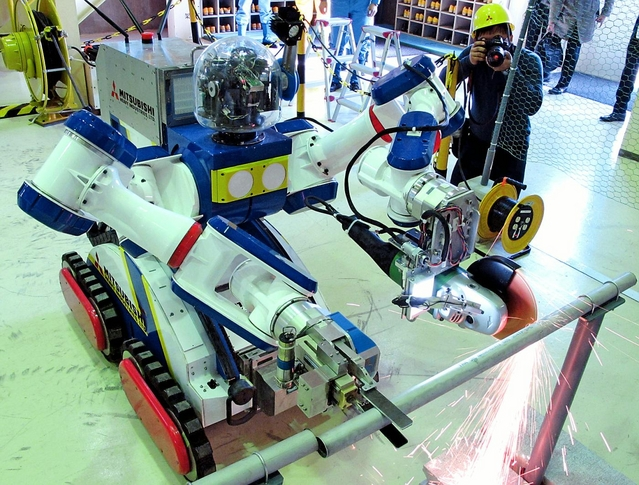
\includegraphics[width=0.8\textwidth]{mhi-meister.jpg}
	\caption[Demonstration of MHI MEISTeR at Fukushima Daiichi NPS]{Demonstration of the tele-operated MHI MEISTeR robot at Fukushima Daiichi Nuclear Power Station \cite{MHI-MEISTeR}}
	\label{FIG:MEISTeR}
	\vspace{-10pt}
\end{figure}
Space and hazardous environments are fruitful environments for cooperative manipulators. Often they are controlled by a human operator from a safe location. Combining human reasoning and the enhanced flexibility of a cooperative set-up is a powerful combination in an unstructured environment. A human in the control loop comes with superior foresight and planning capabilities. To fully exploit this additional flexibility we require control architectures able to perform all the afore-mentioned tasks and operable in a comfortable and efficient manner.\\\\

To address the first requirement the controller realizes changes of formation and relocates the constrained system. A change of formation first of all means the opening and closing of a grasp a around a common object. A virtual object and variable rest-length springs are introduced, the springs couple the virtual and the actual object. The size of virtual object specifies the rest-lengths, by choosing it smaller than the actual a grasping force is exerted. By choosing it bigger the grasp is opened and the actual object is released. Changing of rest-lengths means to change the potential energy stored in the springs. Since the controller itself is passive, the energy is exchanged with a distinct power port. In order to relocate the formation a spring is connected from the virtual object center to the desired new position/orientation. This ensures compliant behavior between (virtual) object and environment. Note that this concept is called \emph{Intrinsically Passive Controller} (IPC) and was introduced by Stramigioli \cite{Stramigioli_01}, the control architecture described in the main part will closely stick to this concept. \\
The controller provides a reasonable layer of abstraction and takes responsibilities from the operator, in order to not overstrain her/his attention and let him focus on important elements of the task. To ensure a secure and stable grasp, the formation of robots is locally controlled without the help of the human. For dynamic manipulation tasks grasp force optimization can be utilized to limit internal to the absolute minimum. The control system provides appropriate feedback to provide better perception on the work environment and to make the job more intuitive. The user specifies system motion and is provided with information about the necessary forces to accomplish the commanded motion. Thereby s/he gets a natural intuition of how much work has been done by the robots. To this end the controller shall never be a source of additional energy, the only way energy is fed into the system is by request of the operator, i.e. the controlled robots are passive. The maximum extractable energy is always bounded, the operator can estimate the stored energy and possible effects when interacting with the environment. Passive robotic systems are always stable when interconnected passive environments/humans and can be stable with some active systems. On the contrary, if the controlled robot is not passive, there is always a passive environment that destabilizes the interconnected system \cite{Stramigioli_15}.



%The major challenge in cooperative manipulation is to simultaneously control the forces between the manipulators and the object, so to say the internal stress exerted on the object, and the forces between the object and the environment, i.e. the absolute motion of the object.
%Strategies that map force and velocity of the object to the manipulators have to be considered.\\
%One important assumption is the nature of the connection between manipulator and object. It can be seen as rigid or more general as friction-based. With a rigid fixture the grasp is always stable, on the contrary friction grasps need to be actively stabilized. To comply with the friction constraints a contact normal force has to be set, dependent on the tangential components present during manipulation.\\
%Towards a versatile usage of cooperative manipulation it is vital to let the human operator control the robotic system intuitively and naturally. 
%A promising approach is gesture control. Gioioso et al. \cite{Gioioso_2014} demonstrated this for a formation of unmanned aerial vehicles. They are able to control opening and closing of the grasp. In a grasped state the objects's pose and the grasping forces can be changed, just by tracking gesture of a single human hand. 
%Directly integrating the human into the control scheme makes use of the visual tracking capacities of the human and eases operation in unknown environments. Regardless of the operator being present on-site with the robots or not, hand tracking and analysis requires a certain time. This delay in the control loop can cause instability. The problem can be modelled as a transmission line with delay and treated with methods known from tele-operation.
%The human takes the role of a supervisor, representing a high-level part of the control scheme. He is responsible for planning, choosing a trajectory and if necessary setting of grasping forces.
%On a local low-level robots need to coordinate their motion compliant with the commanded trajectory and adjust their formation to realize the desired internal forces. For non-rigid fixtures the local robot controller requires the position of the other manipulators. The local communication between the robots causes delay, which has to be treated with tele-operation techniques in order to ensure stability.\\
%Haptic feedback??

 

\section{Problem Statement}

%\textit{You can either state the problem you are trying to solve in the general introduction, providing the transition from the overall picture to your specific approach, or state it in a separate section. Even if you don't use the separate section, writing down in a few sentences why the problem you are trying to solve is actually hard and hasn't been solved before can give you a better idea of how to approach the topic. This can be also merged with the related work part.}\\

Manipulating an unknown object in an unstructured environment is an interesting task for a human-guided cooperative manipulation set-up. Dropping the assumption of a rigid- connection between manipulator and object, the grasp has to be actively stabilized under varying circumstances. During dynamic manipulation a slipping of contact due to the inertia of the object has to be avoided using an automatic mechanism. On the other hand the operator must directly adjust grasp forces for heavy or fragile objects.\\
Position and velocity of the manipulated object are difficult to track in an everyday setting. Usually only end-effector position and velocity of the robots are available. Object position has to be estimated from the known data.\\
For grasping an  object of unknown or even flexible shape, the determination of a fixed grasp map in advance is not useful. Size and shape of the grasp have to be determined by the operator during the grasp process. The controller has to be flexible to varying grasp geometries during the whole task execution.\\
Integrating the human into the control loop, energetic passivity of the closed loop system is a meaningful and intuitive way to ensure stability and a natural way of interaction. Energetic passivity limits the extractable mechanical energy from the closed loop system. This means that the potential damage is also limited. 
Energetic passivity of the robotic system ensures stability of the interconnection stability with any passive systems. Since humans and many relevant environments are passive the closed loop system will always be stable if the overall control scheme is designed energetically passive.


\section{Related Work}
A notable class of control architectures for cooperative manipulation is hybrid position/force control, with a motion control loop for trajectory tracking and a force control loop for internal forces \cite{Wen_92,Hsu_93}. Their drawback is the inability to handle non-contact to contact transitions. Hogan introduced impedance control, which enforces a relation between force and motion \cite{Hogan_84}. Its first application in cooperative manipulation was in \cite{Schneider_92} for realizing compliant object-environment interaction (external impedance control). Bonitz and Hsia \cite{Bonitz_96} applied the concept to the manipulator-object relation (internal impedance control).\\
More recent impedance control schemes can be classified in terms of the information and sensor data available for the problem. Frugal architectures are formation control \cite{Sieber_15} and the static IPC \cite{Wimboeck_06}. Both do not incorporate the object dynamics in control, thus very little knowledge about the object (e.g. dimensions) is necessary. The control loops depend only on relative positions and velocities of the manipulators and do not require object tracking. Neglecting considerable object dynamics is an obvious drawback of the schemes.\\
The concept of the \emph{Intrinsically Passive Controller} (IPC), introduced by Stramigioli \cite{Stramigioli_01} and called dynamic IPC by Wimb\"ock et al. \cite{Wimboeck_08}, tries to overcome some of the limitations. In the controller the object is represented by a virtual pendent and simulated to reproduce its dynamics for control purpose. This has the advantage that still no tracking of the object is required, object velocity and even acceleration can be obtained from the simulation. \\
Techniques which rely on exact knowledge of the object motion were introduced by Caccavale et al. \cite{Caccavale_01,Caccavale_08} and more recent \cite{Heck_13} and \cite{DePascali_15}. It is common to them that they assume rigid fixtures to a rigid object, these conditions overcome the problem of object tracking. The approaches by Caccavale and co-workers use force/torque sensors at the manipulators to establish compliant object environment interaction, for this purpose Heck et al. \cite{Heck_13} assume to have an exact model of the environment. Stramigioli's IPC implements a compliant relation between virtual object and environment. \\
The human operator must be able control the manipulators at a reasonable degree of complexity, therefore in an direct master-slave approach each robot is controlled independently by a human operator. Exactly coordinating their motions is a difficult task for humans, as a consequence a certain amount of autonomy is left to the robot system, enabling a single operator to control the cooperative system. Lee and Spong \cite{Lee_05} apply the master-slave scheme but treat the constrained system as a single slave, while the formation is preserved by the robots autonomously. Many master-slave systems give the operator force-feedback, while s/he commands the motion. This helps the operator compensate for resistances and gives a natural feeling of the interaction with the environment. The structure then is fully bi-directional, ones refers to bilateral telemanipulation \cite{TeleoperationHandbook}. Leader-follower \cite{Sieber_15,Scheggi_14} schemes differ in terms of feedback provided to the operator. Tactile and visual types are non-reactive, i.e. they do not induce operator movements reacting to a back-driving force \cite{Massimino_93}. A purely vision-based architecture is introduced by Gioioso et al. \cite{Gioioso_2014}, hand gestures are used to both control the motion of the constrained system and the opening and closing of a grasp. Control architectures that leave even further autonomy to the robot system and possess a closed local, autonomous control loop, are categorized as supervisory control. They interacts with the operator by continuously sending information about the state and periodically receiving commands \cite{Sheridian_92}.\\
The assumption of rigid fixtures between manipulators and object is very common in cooperative manipulation, Lee and Spong \cite{Lee_05} are an exception. Friction grasps are mainly researched in robot hand literature (\cite{Wimboeck_06,Wimboeck_08,Stramigioli_01}). For the stabilization of a friction grasp it is vital to choose appropriate forces depending on the dynamic state. Therefore the Coulomb friction constraints along with other criteria (safety margins, force limits) can be formulated as a cost function for optimization. Buss et al. \cite{Buss_96} realized that the Coulomb friction constraints can be formulated as positive definite matrices, Han et al. \cite{Han_2000} gave a linear matrix inequality problem. For this type of optimization problems very efficient, real-time solvers exist.
\\


%Control strategies suitable for Cooperative Manipulation can be classified dependent on the nature of the manipulator-object connection: rigid-fixture and friction-grasps.
%An import group within the former are the hybrid position/force control approaches. 
%Control action is decomposed in a motion control loop, accounting for the tracking if the desired trajectory for the overall system and a force control loop to control the internal forces on the object. A pre-defined selection matrix determines for every workspace coordinate whether it is position or force controlled. Controlling the robot on joint level, the necessary torques can be computed using a PD plus gravity compensation control scheme. The desired joint positions and velocities are computed by inverse kinematics \cite{Wen_92}.
%Object level control architectures often use feedback linearisation of the non-linear manipulator dynamics to achieve a linear and decoupled control of motion and grasping force \cite{Hsu_93}.
%Force control is only meaningful if contact between manipulator and object. Motion control leads to unbounded forces if the motion direction is not consistent with the constraints,  since force in this direction is not controlled. The transition between contact and no contact during grasping cannot be handled with these approaches. For these reasons in the following only the better suited impedance control schemes are considered. Impedance control, introduced by Hogan \cite{Hogan_84}, is a well known strategy to avoid unbounded forces when it comes to interaction of manipulators with objects/environment. It does not control one state variable (position, velocity, force) dynamically enforces a relation between forces and system state. Contact directions do not have to be pre-specified. The controller is stable independently of the contact state.
%A physical analogy the impedance control scheme is a spring-mass-damper system.\\  

%\textit{From Kevin Elphinstone's \emph{A Small Guide to Writing Your Thesis}\cite{Elphinstone2014}:}
%
%\textit{"The related work section (sometimes called literature review) is just that, a review of work related to the problem you are attempting to solve. It should identify and evaluate past approaches to the problem. It should also identify similar solutions to yours that have been applied to other problems not necessarily directly related to the one your solving. Reviewing the successes or limitations of your proposed solution in other contexts provides important understanding that should result in avoiding past mistakes, taking advantage of previous successes, and most importantly, potentially improving your solution or the technique in general when applied in your context and others.}

%\textit{In addition to the obvious purpose indicated, the related work section also can serve to:}

%\begin{itemize}
%	\item \textit{justify that the problem exists by example and} argument
%	\item \textit{motivate interest in your work by demonstrating relevance and importance}
%	\item \textit{identify the important issues}
%	\item \textit{provide background to your solution}
%\end{itemize}

%\textit{Any remaining doubts over the existence, justification, motivation, or relevance of your thesis topic or problem at the end of the introduction should be gone by the end of related work section.}

%\textit{Note that a literature review is just that, a review. It is not a list of papers and a description of their contents! A literature review should critique, categorize, evaluate, and summarize work related to your thesis. Related work is also not a brain dump of everything you know in the field. You are not writing a textbook; only include information directly related to your topic, problem, or solution."}

%\textit{Note: Do the literature review at an early stage of your project to build on the knowledge of others, not reinvent the wheel over and over again! There is nothing more frustrating after weeks or months of hard work to find that your great solution has been published 5 years ago and is considered old news or that there is a method known that produces superior results.}

%\subsection{Control schemes for rigidly connected manipulators}\label{SS:rigidcontrolschemes}
%A rigid fixture between manipulator and object means that both forces and moments are exchanged at the grasp points: all translational and rotational motion components can be transmitted through the contact points. The rigid connections are expressed by a number of kinematic constraints, which reduce the Degrees-of-Freedom (DoF) of the constrained system. The attempt to move in the constrained directions results in internal loading of the object. Therefore trajectories of the manipulators have to be generated to avoid internal stress on the object. Assuming a rigid connection normally no grasping force is needed to stabilize the grasp, i.e. internal forces are undesired because possibly harmful to the object. Nevertheless some papers propose possibilities to specify or control internal forces.\\
%Among the first to use impedance control in cooperative manipulation were Schneider and Cannon \cite{Schneider_92}. They replaced the actual object by a virtual mass and connected it to the environment with a spring and a parallel damper. The resulting impedance equation is:
%\begin{equation}
%M_{o,d} (\ddot{x}_o^d - \ddot{x}_o) + D_o (\dot{x}_o^d - \dot{x}_o) + K_o(x_o^d,x_o) = h_{env} 
%\end{equation}
%Here $ M_{o,d} $ denotes the inertia of the virtual object, $ D_o $ is the damping along the spring, which is represented by $ K_o(x_d,x) $. $ x_o = (p_o^T,Q_o^T)^T $ is the stacked vector of position and orientation of the object. $ x^d $ denotes a desired quantity. The external wrench, exerted by the environment on the object, $ h_{env} = (f_{env}^T,t_{env}^T)^T$ consists of force and torque vectors.
%The dynamics of the virtual object is then given as:
%\begin{equation}
%M_{o,d}\ddot{x} = -h_{env} + h_o^{\Sigma} = -h_{env} + M_{o,d}\ddot{x}_d + D_o (\dot{x}_d - \dot{x}) + K_o(x_d,x)
%\end{equation}
%The resulting impedance control output $ h_o^{\Sigma} $ is than mapped to the manipulators using a generalized inverse of the grasp matrix:
%\begin{equation}
%h^{\Sigma} = G^\dagger h_o^{\Sigma}
%\end{equation}
%Performance of this strategy depends on choosing the virtual inertia close to the actual, i.e. good knowledge of the object is required. Furthermore gravity compensation would be necessary to model the full object dynamics. In general the equation of motion for a rigid object is:
%\begin{equation}\label{EQ:ObjectDynamics}
%M_o \ddot{x}_o + C_o \dot{x}_o + g_o = h_{env} + h^\Sigma
%\end{equation}
%Wherein $ M_o $ is the actual object inertia, $ C_o $ is the Matrix accounting for the Coriolis force and $ g_o $ is the gravity. 
%For notational convenience the pose dependencies of the parameter matrices, e.g. $ M_o(x_o) $, are omitted.\\
%Bonitz and Hsia \cite{Bonitz_96} propose to model each manipulator as an impedance relation. Thereby a relation between manipulator dynamics and internal forces on the object is enforced:
%\begin{equation}
%M_i(\ddot{x}_i^d - \ddot{x}_i) + D_i (\dot{x}_i^d - \dot{x}_i) + K_i(x_i^d,x_i) = h_{int}
%\end{equation}
%$ M_i, D_i, K_i(x_i^d,x_i) $ are the desired inertia, damping and stiffness representations of the i-th manipulator.The internal wrench $ h_{int} = VV^\dagger h $ is calculated from the measured contact wrench $ h $. $ V $ is a basis of the nullspace of the grasp matrix, $ V^\dagger $ denotes the pseudoinverse. No assumptions on the object are necessary because it is not considered in the control scheme.\\ 
%The first approach ensures compliant object-environment interaction, while the second limits internal forces even in case of end-effector displacements. The both have been combined by Caccavale and Villani \cite{Caccavale_01}. Their control architecture is cascaded, consisting of a two level reference trajectory generation and a motion control loop below. On top-level an impedance relation between object and environment is used to generate a compliant trajectory subject to environmental forces:
%\begin{equation}
%\alpha M_o(\ddot{x}_o^d - \ddot{x}_o^r)  + D_o(\dot{x}_o^d - \dot{x}_o^r) + K_o(x_o^d,x_o^r)  = h_{env}
%\end{equation}
%The constant $ \alpha $ scales the object inertia proportionally to a desired value.
%The control output is the reference object acceleration $ \ddot{x}_o^r $, $ h_{env} $ is an input. This is sometimes called admittance control, admittance being the inverse of impedance. $ h_{env} $ has to be known, but is not easily measured in a practical set-up. Recalling (\ref{EQ:ObjectDynamics}) the environmental forces can be expressed as:
%\begin{equation}
%h_{env} =  M_o \ddot{x}_o^r + C_o \dot{x}_o^r + g_o - G^\dagger h
%\end{equation}
%Herein $ G^\dagger $ is a generalized inverse of the grasp matrix, selecting the motion inducing components from the measured contact wrench $ h $. $ \dot{x}_o^r, x_o^r $ are calculated from $ \ddot{x}_o^r $ by integration.
%From the compliant object trajectory ($ \ddot{x}_o^r,\dot{x}_o^r,x_o^r $) the desired trajectories of the manipulator ($ \ddot{x}_i^d,\dot{x}_i^d,x_i^d $) using the kinematic constraints. The reference manipulator trajectory, enforcing compliant behaviour between manipulators and object, is calculated from manipulator dynamics and internal forces: 
%\begin{equation}
%M_i(\ddot{x}_i^d - \ddot{x}_i^r) + D_i (\dot{x}_i^d - \dot{x}_i^r) + K_i(x_i^d,x_i^r) = VV^\dagger h
%\end{equation}
%The control output is the reference acceleration of the i-th manipulator $ \ddot{x}_i^r $, $ \dot{x}_i^r,x_i^r $ are obtained from integration. These variables are the inputs the inner motion control loop (PD-type). The strategy of compliant trajectories allows for high gains in the motion controller. Knowledge of object dynamics and measurement of the contact wrenches is required.\\
%In a frequently cited follow-up paper Caccavale et al. \cite{Caccavale_08} combine the concept of \emph{geometrically consistent stiffness} with the same architecture. This allows for selective stiffness behaviour along different directions.\\
%Recently Heck et al. \cite{Heck_13} worked with this architecture, they assume knowledge of the environment instead of the object.
%The environmental wrench is than derived as:
%\begin{equation}
%h_{env} =  \Sigma D_{env} (\dot{x}_o^d - \dot{x}_o^r)  + \Sigma K_{env}(x_o^d,x_o^r)
%\end{equation}
%It is assumed here that the environment has a constant stiffness and damping ($ K_{env}(x_o^d,x_o^r),D_{env}) $. $ \Sigma $ is a diagonal selection matrix modelling the direction of contact.\\
%A combination of impedance control on manipulator/object level and feed-forward object dynamics is presented in\cite{DePascali_15}. The manipulators are modelled as springs and dampers, inertia is used to feed-forward the desired acceleration: 
%\begin{equation}
%M_i \ddot{x}_i^d + D_i (\dot{x}_i^d - \dot{x}_i) + K_i(x_i^d,x_i) = h^x
%\end{equation}
%This avoids the necessity of either measuring manipulator acceleration or contact force.
%Object dynamics is represented with feed-forward term, mapped to the manipulators with a weighted pseudoinverse $ G^+ $ of the grasp matrix:
%\begin{equation}
%h^d = G^+ (M_o \ddot{x_o^d} + C_o \dot{x_o^d} + g_o)
%\end{equation}
%Note that this term is not an impedance relation and does not adjust if the environment hinders motion.
%The combined control law is $ h^\Sigma = h^x + h^d $.\\
% 
%
%
%\subsection{Friction grasps in Cooperative Manipulation}
%The assumption of rigid-fixture between object and manipulators only holds f the manipulators are equipped with  appropriate grasping devices. In analogy to a human this device would be fingers wrapping around an inhomogeneity on the object, to achieve a rigid grasp. For an even object (e.g. a ball) humans use their hand palms to realize a friction grasp. Grasp stability is ensured by pressing the object. Technical applications where cooperative manipulators should be able to do a friction grasp are numerous, e.g. when no appropriate grasping device is available (or shall be avoided) or the object structure is not graspable.\\
%Research of friction grasps is mainly done with robotic hands, the fingertips being the contact points. Depending on the nature of the tip a certain number of contacts is required to achieve a firm grasp: for non-deformable and small but frictional contacts, three are required to hold an object with 6 \emph{DoF} tightly. This contact model is called \emph{Hard Finger} or \emph{Point Contact with Friction (PCwF)}. It allows to transmit forces along the contact normal in pushing direction and for forces in tangential plane. If the contact is deformable or of considerable size, two are sufficient contact points form a firm grasp. This is called \emph{Soft Finger} model. In addition to the \emph{Hard Finger} torques around the contact normal are transferred.\\
%The problem of grasping divides into three sub-problems: selection of suitable grasp points, coordinated motion of the constrained system and control of the grasping force especially when interacting with the environment. The problem of coordinated motion is very similar to the case of rigid-fixture, while the control is exclusive to friction grasps. With robot hands it is most important to maintain a stable grasp. Undesired or unnecessary and possibly harmful internal forces occur during dynamic manipulation and interaction with the environment. Since discrete robots in cooperative manipulation are often powerful, proper control of the internal forces becomes more important.\\
%For the reasons stated in the previous subsection hybrid position/force control approaches are less suitable than impedance control and will not be considered. The control architectures for rigid-fixture can be re-used if a internal force is applied in addition. By definition internal forces do not contribute to the motion of the constrained system and thus do not interfere with the control goals of rigid-fixture. Formally this can be described as $ G h_{int} = 0 $, i.e. the internal forces $ h_{int} $ lie in the null-space of the grasp matrix $ G $. To calculate desired internal forces a suitable vector $ z $ is multiplied with a basis of the null-space of the grasp matrix $ V $: $ h_{int}^d = V z $.\\
%When it comes to position uncertainties of contact points or deformable objects, calculating internal forces from a fixed grasp matrix may lead to undesired results. One alternative are \emph{Artificial Potential Fields (AFP)} to realize a desired formation of manipulators relative to each other in 3D space. 
%Sieber et al.\cite{Sieber_15} use \emph{AFP} to build up a formation of robots around an object. The object is grasped by varying the desired distances between the manipulators. The internal forces can thus be set in a physically meaningful way. The generated force of manipulator $ i $ in Cartesian direction $ k $ due to the springs connecting to the other manipulators $ j \in N_i $ is:
%\begin{equation}
%f_{i,k}^d = - \sum_{\substack{j\in N_i}} k_{ij} \dfrac{p_{i,k} - p_{j,k}}{\vert p_{i,k} - p_{j,k} \vert} (\vert p_{i,k}-p_{j,k}\vert - d_{ij,k})
%\end{equation}
%Notably here $ p\in\mathbb{R}^3 $ only represents the position of the manipulator, orientation information is omitted. Using the \emph{Hard Finger} contact model a pure translational representation is sufficient since it does not transmit torques. $ k_{ij} > 0$ is a control gain. The desired distance is defined by $ d_{ij,k} $.
%The approach controls only the formation of the robots and does not take the object dynamics into account. Positional control for the object is done assuming the object to be in the middle of the manipulators: $ p_o = \frac{1}{N} \sum\nolimits_{i=1}^{N} x_i $. This has important advantages: no need to know the object's dynamics and no need for tracking the object.\\
%Similar to the concept of \emph{AFP} are 1-\emph{DoF} springs with a desired rest-length. They only allow to set the absolute distance between two points in space, while \emph{AFP} control the distance along each direction. 1-\emph{DoF} can be more intuitive to control, because only one distance parameter has to be changed in contrast to a relative formation in 3D space.\\
%One approach using 1-\emph{DoF} springs is the \emph{Static IPC} by Wimb\"ock et al. \cite{Wimboeck_06}. The concept of the \emph{intrisically passive controller (IPC)} was introduced by Stramigioli \cite{Stramigioli_01} and will be covered later on. Here the rest-length springs connect to the middle of the manipulator set-up. The force generated by a single spring connecting from manipulator $ i $ to the center is: $ k_{i} \frac{p_i - p_o}{\vert p_i - p_o \vert} (\vert p_i-p_o\vert - d_{i}) $. Here $ k_i \in \mathbb{R}^3 $ is the stiffness matrix and $ d_i $ is the rest-length of the $ i $-th spring.
%Considering the cross-coupling of the springs the generated forces are:
%\begin{equation}
%f^d  = - \sum_{i=1}^N\left[\dfrac{\partial (p_i-p_o)^T}{\partial p} k_i \dfrac{p_i-p_o}{\vert p_i-p_o\vert}  (\vert p_i-p_o\vert - d_i) \right]
%\end{equation}
%Wherein $ \frac{\partial (p_i-p_o)^T}{\partial p} \in \mathbb{R}^{3N \times 3} $ is the cross-coupling matrix.
%Furthermore this approach uses another spring to connect environment and object. This is a 6-\emph{DoF} spring, thus the object's position and orientation is controlled. Force and torque are computed as:
%\begin{subequations}
%\begin{align}
%f_o^d = K_{o,t} R_o^T (p_o-p_o^d) \\
%t_o^d = 4 J^T_{\omega\epsilon} K_{o,r} \epsilon_d 
%\end{align}
%\end{subequations}
%The translational and rotational stiffness matrices are denoted by $ K_{o,t},K_{o,r} $. $ R_o $ is a rotation matrix indicating the object orientation, it is defined by the manipulator positions. $ \epsilon_d $ is the rotational error represented by the vector part of the quaternion, $ J^T_{\omega\epsilon} $ denotes the reduced quaternion product.\\
%Damping along each spring is proposed. This important especially for the cross-coupling springs to suppress oscillatory internal motions.\\
%While $ f^d $ acts on the manipulators, $ f_o^d $ and $ t_o^d $ act on the object. This is resolved by the hand geometry, different hand \emph{Jacobian} matrices cast the wrenches into joint torques. If no kinematic structure is present (e.g. when using discrete robots) often a weighted pseudoinverse of the grasp matrix (\cite{Schneider_92,DePascali_15}) is used. According to Stramigioli\cite{Stramigioli_01} the physically meaning of the weighting coefficients is small. Erhart and Hirche\cite{Erhart_15} recently presented weighted pseudoinverses based on inertia and geometry of object and manipulators. However (in some cases) this requires konwledge of the object properties. Stramigioli therefore introduces a virtual object, the wrench acts directly onto the virtual object and thus  influences its dynamics. The manipulators are connected to the virtual object with rest-length springs, so the object wrench is mapped to the manipulators via the virtual object dynamics.
%Wimb\"ock et al. implement Stramigioli's \emph{IPC} in a simplified version on a four fingered robotic hand\cite{Wimboeck_08}. The dynamics of the virtual object are:
%\begin{equation}
%M_v \ddot{x}_v + C_v \dot{x}_v + g_v = w_v
%\end{equation}
%The virtual object wrench $ w_v $ is composed of environment interaction $ w_{vo} $ and manipulator forces $ f_c $: $ w_v = w_{vo} + G_v f_c $. Where $ G_v $ is the virtual grasp matrix. Environment interaction is described by a 6 \emph{DoF} spring: $ w_{vo} = K(x_v^d,x_v) $. The springs connecting to the manipulators exert the wrench on the virtual object: $ G_v f_c = G_v K_c (p - G_v^T x_v) $. The control law for the manipulators is already given as:
%\begin{equation}
%f = -f_c = K_c(G_v^T x_v - p)
%\end{equation}
%The stiffness matrix $ K_c = blockdiag(k_1 I_3, ... , k_n I_3)$ is isotropic. The rest-lengths of the springs are chosen by the size of the virtual object, i.e. by specifying the virtual grasp matrix $ G_v $.\\
%One assumption in \cite{Wimboeck_08} is that internal forces are sufficient to ensure a firm grasp. This is done in a physically meaningful way by choosing the rest-lengths.
%Allowing a human to directly control the formation (e.g. with gestures), three parameters are to be specified by the operator: position, orientation and grasping force. Tracking and processing human inputs causes a delay, which can be compared to a telemanipulation setting, although the operator may be on-site. A local controller is required to ensure a secure grasp while human interfacing can be higher level control.

%\subsection{Determination of desired internal forces}
%Non-rigid grasps object and manipulators are connected with friction constraints. Contact force towards the object generates frictional force opposed to external forces tangential to the contact point. If the tangential forces exceed the frictional force the friction constraint is violated and contact slippage occurs. Squeezing or internal forces do not contribute to the motion of the constrained system. They need to be chosen sufficiently high to maintain a stable grasp under external forces acting on the object. On the other hand they must be bounded to not damage the object. These opposed requirements can be formulated as a cost function.\\
%Buss et al. \cite{Buss_96} propose a cost function consisting of two factors: one is a barrier function tending to infinity for violating the friction constraint limit, the other is linear function rising with the exerted force, making high forces costly. The optimal desired internal force is the minimum of the cost function, thus the forces are chosen as small as possible, preserving a stale grasp.\\
%Non-linear friction constraints are given for the \textit{point contact friction} and the \textit{soft contact friction} model:\\
%The \textit{point contact friction} constraint allows transmitting force in tangential  and normal  (only towards the object) direction. In addition the \textit{soft contact} constraint transmits the torsional moment around the normal axes. Buss' main contribution is that friction constraints can be reformulated  equivalent to positive definite matrices. These matrices are used to construct the cost function. This results in a convex optimization problem, thus an optimum is always a global optimum. \\
%Bicchi et al. \cite{Bicchi_98} limit their contribution to the \textit{point contact friction} model but expand the cost function. A maximum contact force is introduced, this is useful for rather loosing contact than destroying the object. Furthermore a minimum force in normal direction is specified to ensure grasp stability even under uncertainties. This two add up to with the friction constraint to a function, which has a negative scalar value if the set of constraints are respected. The sum of this functions for all contact points forms the cost function.\\ 
%Han et al. \cite{Han_2000} reformulated Buss' positive definite matrix approach as a \textit{linear matrix inequality}(LMI) problem. Being a common optimization task, efficient solvers (e.g. interior point algorithm) exist. Calculation time could be significantly reduced.
%____________________________________________________



%_____Kapitel 2_________________________________
\chapter{port-Hamiltonian system modelling}
%The controller is divided into two parts, the local one does the real-time interaction of the manipulators with the object. This part is passive, i.e. the robot along with its local controller has a certain amount of energy, the energy can not increase as long as no power is provided by the environment or the higher-level control part. Therefore the two parts will be called Intrinsically Passive Controller and Supervisor, this scheme was introduced by Stramigioli \cite{Stramigioli_01} as a general framework with application to robotic hands.
In this chapter a modelling approach of the cooperative   system based on the port-Hamiltonian framework is introduced. This aims for a consistent system description over different energetic domains, present in mechanical systems in the form of kinetic and potential energy. The general theory of port-Hamiltonian systems is presented in Section \ref{S:HSdescription}. The generalization for six-dimensional mechanical system leading to systems defined on manifolds is introduced in Section \ref{S:3Dspace-modelling}. In cooperative manipulation set-ups, manipulators and object are rigidly connected, the arising constraints are treated in Section \ref{SS:ImposingConstraints}. 
System modelling is performed by interconnecting standardized mechanical elements using network theory. The composition of a mechanical impedance, suitable for model-based control (see Chapter 3) is shown in Section \ref{S:springmassdampers}.
  


\section{port-Hamiltonian description of mechanical systems}\label{S:HSdescription}
For the derivation of the port-Hamiltonian description of a mechanical system we start from the classical \emph{Euler-Lagrange} equations of motion
\begin{equation}
\frac{d}{dt}\left(\frac{\partial \mathcal{L}}{\partial \dot{q}}\right) - \frac{\partial \mathcal{L}}{\partial q} = g(q)f,
\end{equation}
where $q$ is the vector of generalized configuration coordinates of the system. The \emph{Lagrangian} $\mathcal{L} = V_k - V_p$ equals the difference between the kinetic co-energy $V_k$ and the potential energy $V_p$. The kinetic co-energy is explicitly given as $V_k = \frac{1}{2} \dot{q}^T M(q) \dot{q}$, with a symmetric, positive definite inertia matrix $M(q)$. The generalized forces $f$ act on the system with an input matrix $g(q)$. We define the generalized \emph{momenta} for every Lagrangian $p := \frac{\partial \mathcal{L}}{\partial \dot{q}}$ and obtain $p = M(q)\dot{q}$.
Introducing the \emph{Hamiltonian} (energy) function $H(q,p) = p^T\dot{q} - \mathcal{L}(q,\dot{q})$ we can rewrite the Euler-Lagrange equation in form of the classical Hamiltonian equations of a mechanical system \begin{eqnarray}\label{EQ:generalPHS}
	\begin{aligned}
	& \dot{q} = \frac{\partial H}{\partial p}(q,p)\\
	& \dot{p} = -\frac{\partial H}{\partial q}(q,p) + g(q)f
	\end{aligned}
\end{eqnarray}
The Hamiltonian describes the total energy stored in the system \cite{vanderSchaft_06}, thus the energy balance is
\begin{equation}
	\frac{d}{dt}H = \frac{\partial^T H}{\partial q}(q,p)\dot{q} + \frac{\partial^T H}{\partial p}(q,p)\dot{p} = f^Tg^T(q)\dot{q} = f^Te
\end{equation}
Hamiltonian systems are energy conservative, i.e. the energy supplied through the port is stored in the system. In the upper equation a new output $e=g^T(q)\dot{q}$ is introduced. Clearly the product $e^Tf$ is the exchanged power and we call the pair $(f,e)$ a \emph{power port}.
The general equations of a port-Hamiltonian system are
\begin{eqnarray}
\begin{aligned}
	& \dot{q} = \frac{\partial H}{\partial p}(q,p)\\
	& \dot{p} = -\frac{\partial H}{\partial q}(q,p)+g(q)f \\   &e = g^T(q)\frac{\partial H}{\partial p}(q,p)
\end{aligned}	
\end{eqnarray}
Port-Hamiltonian systems are suitable to describe a variety of physical systems including mechanical, electrical, thermal and hydraulic elements, see \cite{duindam2009geoplexbook} for an overview. This motivates the more general input-output concept of flows $f$ and efforts $e$ forming the port variables $(f,e)$.\\
\textbf{Example 2.1:}\\
Consider a simple one-dimensional spring-mass system described by $ m\ddot{x} = -kx +F $, where $ m,k,F $ denote the mass, stiffness and external force acting on the mass respectively. We can give a state space formulation of the system
\begin{figure}[b!]
	\centering
	\sf\small
	\def\svgwidth{0.5\columnwidth}
	%LaTeX with PSTricks extensions
%%Creator: 0.91_64bit
%%Please note this file requires PSTricks extensions
\psset{xunit=.5pt,yunit=.5pt,runit=.5pt}
\begin{pspicture}(744.09448819,1052.36220472)
{
\newrgbcolor{curcolor}{1 1 1}
\pscustom[linestyle=none,fillstyle=solid,fillcolor=curcolor]
{
\newpath
\moveto(433.9839592,679.23058241)
\curveto(433.9839592,660.64698979)(418.9189808,645.5820114)(400.33538818,645.5820114)
\curveto(381.75179557,645.5820114)(366.68681717,660.64698979)(366.68681717,679.23058241)
\curveto(366.68681717,697.81417503)(381.75179557,712.87915342)(400.33538818,712.87915342)
\curveto(418.9189808,712.87915342)(433.9839592,697.81417503)(433.9839592,679.23058241)
\closepath
}
}
{
\newrgbcolor{curcolor}{0 0 0}
\pscustom[linewidth=1.5,linecolor=curcolor]
{
\newpath
\moveto(433.9839592,679.23058241)
\curveto(433.9839592,660.64698979)(418.9189808,645.5820114)(400.33538818,645.5820114)
\curveto(381.75179557,645.5820114)(366.68681717,660.64698979)(366.68681717,679.23058241)
\curveto(366.68681717,697.81417503)(381.75179557,712.87915342)(400.33538818,712.87915342)
\curveto(418.9189808,712.87915342)(433.9839592,697.81417503)(433.9839592,679.23058241)
\closepath
}
}
{
\newrgbcolor{curcolor}{0 0 0}
\pscustom[linewidth=1.5,linecolor=curcolor]
{
\newpath
\moveto(144.85715,678.81484472)
\lineto(158.74845,678.81484472)
\curveto(158.74845,678.81484472)(163.37889,697.33658472)(181.90063,697.33658472)
\curveto(191.1615,697.33658472)(195.79193,682.59527472)(195.79193,678.81484472)
\curveto(195.79193,674.18441472)(195.79193,660.37820472)(186.53106,660.29311472)
\curveto(181.90083,660.25051472)(177.27019,669.38803472)(177.27019,678.81484472)
\curveto(177.27019,688.07571472)(181.90063,697.33658472)(195.79193,697.33658472)
}
}
{
\newrgbcolor{curcolor}{0 0 0}
\pscustom[linewidth=1.5,linecolor=curcolor]
{
\newpath
\moveto(195.79193,697.33658472)
\curveto(209.68324,697.33658472)(214.31367,682.59527472)(214.31367,678.81484472)
\curveto(214.31367,674.18441472)(214.31367,660.37820472)(205.0528,660.29311472)
\curveto(200.42256,660.25051472)(195.79193,669.38803472)(195.79193,678.81484472)
\curveto(195.79193,688.07571472)(200.42237,697.33658472)(214.31367,697.33658472)
}
}
{
\newrgbcolor{curcolor}{0 0 0}
\pscustom[linewidth=1.5,linecolor=curcolor]
{
\newpath
\moveto(214.31367,697.33658472)
\curveto(228.20498,697.33658472)(232.83541,682.59527472)(232.83541,678.81484472)
\curveto(232.83541,674.18441472)(232.83541,660.37820472)(223.57454,660.29311472)
\curveto(218.9443,660.25051472)(214.31367,669.38803472)(214.31367,678.81484472)
\curveto(214.31367,688.07571472)(218.94411,697.33658472)(232.83541,697.33658472)
}
}
{
\newrgbcolor{curcolor}{0 0 0}
\pscustom[linewidth=1.5,linecolor=curcolor]
{
\newpath
\moveto(232.83541,697.33658472)
\curveto(246.72672,697.33658472)(251.35715,682.59527472)(251.35715,678.81484472)
\curveto(251.35715,674.18441472)(251.35715,660.37820472)(242.09628,660.29311472)
\curveto(237.46604,660.25051472)(232.83541,669.38803472)(232.83541,678.81484472)
\curveto(232.83541,688.07571472)(237.46585,697.33658472)(251.35715,697.33658472)
}
}
{
\newrgbcolor{curcolor}{0 0 0}
\pscustom[linewidth=1.5,linecolor=curcolor]
{
\newpath
\moveto(251.35715,697.33658472)
\curveto(265.24845,697.33658472)(269.87889,682.59527472)(269.87889,678.81484472)
\curveto(269.87889,674.18441472)(269.87889,660.37820472)(260.61802,660.29311472)
\curveto(255.98778,660.25051472)(251.35715,669.38803472)(251.35715,678.81484472)
\curveto(251.35715,688.07571472)(255.98758,697.33658472)(269.87889,697.33658472)
}
}
{
\newrgbcolor{curcolor}{0 0 0}
\pscustom[linewidth=1.5,linecolor=curcolor]
{
\newpath
\moveto(269.87889,697.33658472)
\curveto(283.77019,697.33658472)(288.40063,682.59527472)(288.40063,678.81484472)
\curveto(288.40063,674.18441472)(288.40063,660.37820472)(279.13976,660.29311472)
\curveto(274.50952,660.25051472)(269.87889,669.38803472)(269.87889,678.81484472)
\curveto(269.87889,688.07571472)(274.50932,697.33658472)(288.40063,697.33658472)
}
}
{
\newrgbcolor{curcolor}{0 0 0}
\pscustom[linewidth=1.5,linecolor=curcolor]
{
\newpath
\moveto(288.40063,697.33658472)
\curveto(302.29193,697.33658472)(306.92237,682.59527472)(306.92237,678.81484472)
\curveto(306.92237,674.18441472)(306.92237,660.37820472)(297.6615,660.29311472)
\curveto(293.03126,660.25051472)(288.40063,669.38803472)(288.40063,678.81484472)
\curveto(288.40063,688.07571472)(293.03106,697.33658472)(306.92237,697.33658472)
}
}
{
\newrgbcolor{curcolor}{0 0 0}
\pscustom[linewidth=1.5,linecolor=curcolor]
{
\newpath
\moveto(357.85715,678.81484472)
\lineto(343.96585,678.81484472)
\curveto(343.96585,678.81484472)(339.33541,697.33658472)(320.81367,697.33658472)
\curveto(311.5528,697.33658472)(306.92237,688.07571472)(306.92237,678.81484472)
\curveto(306.92237,674.18441472)(306.92237,660.29311472)(316.18324,660.29311472)
\curveto(320.81367,660.29311472)(325.44411,669.38803472)(325.44411,678.81484472)
\curveto(325.44411,688.07571472)(320.81367,697.33658472)(306.92237,697.33658472)
}
}
{
\newrgbcolor{curcolor}{0 0 0}
\pscustom[linewidth=1.5,linecolor=curcolor]
{
\newpath
\moveto(144.82296,644.79884472)
\lineto(144.82296,714.99972472)
}
}
{
\newrgbcolor{curcolor}{1 1 1}
\pscustom[linestyle=none,fillstyle=solid,fillcolor=curcolor]
{
\newpath
\moveto(365.97257495,678.80568617)
\curveto(365.97257495,676.63421108)(364.21224658,674.8738827)(362.04077148,674.8738827)
\curveto(359.86929639,674.8738827)(358.10896802,676.63421108)(358.10896802,678.80568617)
\curveto(358.10896802,680.97716126)(359.86929639,682.73748963)(362.04077148,682.73748963)
\curveto(364.21224658,682.73748963)(365.97257495,680.97716126)(365.97257495,678.80568617)
\closepath
}
}
{
\newrgbcolor{curcolor}{0 0 0}
\pscustom[linewidth=1.5,linecolor=curcolor]
{
\newpath
\moveto(365.97257495,678.80568617)
\curveto(365.97257495,676.63421108)(364.21224658,674.8738827)(362.04077148,674.8738827)
\curveto(359.86929639,674.8738827)(358.10896802,676.63421108)(358.10896802,678.80568617)
\curveto(358.10896802,680.97716126)(359.86929639,682.73748963)(362.04077148,682.73748963)
\curveto(364.21224658,682.73748963)(365.97257495,680.97716126)(365.97257495,678.80568617)
\closepath
}
}
{
\newrgbcolor{curcolor}{0 0 0}
\pscustom[linewidth=1.5,linecolor=curcolor]
{
\newpath
\moveto(137,715.00000472)
\lineto(145,708.00000472)
}
}
{
\newrgbcolor{curcolor}{0 0 0}
\pscustom[linewidth=1.5,linecolor=curcolor]
{
\newpath
\moveto(137,708.00000472)
\lineto(145,701.00000472)
}
}
{
\newrgbcolor{curcolor}{0 0 0}
\pscustom[linewidth=1.5,linecolor=curcolor]
{
\newpath
\moveto(137,701.00000472)
\lineto(145,694.00000472)
}
}
{
\newrgbcolor{curcolor}{0 0 0}
\pscustom[linewidth=1.5,linecolor=curcolor]
{
\newpath
\moveto(137,694.00000472)
\lineto(145,687.00000472)
}
}
{
\newrgbcolor{curcolor}{0 0 0}
\pscustom[linewidth=1.5,linecolor=curcolor]
{
\newpath
\moveto(137,687.00000472)
\lineto(145,680.00000472)
}
}
{
\newrgbcolor{curcolor}{0 0 0}
\pscustom[linewidth=1.5,linecolor=curcolor]
{
\newpath
\moveto(137,680.00000472)
\lineto(145,673.00000472)
}
}
{
\newrgbcolor{curcolor}{0 0 0}
\pscustom[linewidth=1.5,linecolor=curcolor]
{
\newpath
\moveto(137,673.00000472)
\lineto(145,666.00000472)
}
}
{
\newrgbcolor{curcolor}{0 0 0}
\pscustom[linewidth=1.5,linecolor=curcolor]
{
\newpath
\moveto(137,666.00000472)
\lineto(145,659.00000472)
}
}
{
\newrgbcolor{curcolor}{0 0 0}
\pscustom[linewidth=1.5,linecolor=curcolor]
{
\newpath
\moveto(137,659.00000472)
\lineto(145,652.00000472)
}
}
{
\newrgbcolor{curcolor}{0 0 0}
\pscustom[linewidth=1.5,linecolor=curcolor]
{
\newpath
\moveto(137,652.00000472)
\lineto(145,645.00000472)
}
}
{
\newrgbcolor{curcolor}{0 0 0}
\pscustom[linestyle=none,fillstyle=solid,fillcolor=curcolor]
{
\newpath
\moveto(442.23874,683.17562062)
\lineto(434,680.65661472)
\lineto(442.23874,678.13760882)
\closepath
}
}
{
\newrgbcolor{curcolor}{0 0 0}
\pscustom[linewidth=1.68894935,linecolor=curcolor]
{
\newpath
\moveto(442.15625,680.81250472)
\lineto(473.5343,680.81250472)
}
}
{
\newrgbcolor{curcolor}{0 0 0}
\pscustom[linestyle=none,fillstyle=solid,fillcolor=curcolor]
{
\newpath
\moveto(481.57217407,678.58635634)
\curveto(481.57217407,677.95565972)(481.32599894,677.43075738)(480.83364868,677.0116493)
\curveto(480.34129842,676.59661024)(479.69636027,676.35043511)(478.89883423,676.27312391)
\lineto(478.89883423,674.06365126)
\lineto(478.17861938,674.06365126)
\lineto(478.17861938,676.24260634)
\curveto(477.64151001,676.24667535)(477.13695272,676.29753798)(476.66494751,676.39519423)
\curveto(476.1929423,676.49691949)(475.78400675,676.62712782)(475.43814087,676.78581923)
\lineto(475.43814087,677.99431532)
\lineto(475.53579712,677.99431532)
\curveto(475.61310832,677.93734917)(475.75145467,677.85393446)(475.95083618,677.74407118)
\curveto(476.15021769,677.63827691)(476.34349569,677.55079318)(476.53067017,677.48162001)
\curveto(476.74225871,677.40430881)(476.98843384,677.33106662)(477.26919556,677.26189345)
\curveto(477.55402629,677.19678928)(477.85716756,677.15813368)(478.17861938,677.14592665)
\lineto(478.17861938,679.78874891)
\curveto(478.01585897,679.821301)(477.86530558,679.85181858)(477.72695923,679.88030165)
\curveto(477.58861287,679.91285373)(477.46043905,679.94540581)(477.34243774,679.9779579)
\curveto(476.67918905,680.14478733)(476.20311483,680.39503147)(475.91421509,680.72869032)
\curveto(475.62531535,681.06641818)(475.48086548,681.48145725)(475.48086548,681.97380751)
\curveto(475.48086548,682.57602105)(475.71686808,683.08464735)(476.18887329,683.49968641)
\curveto(476.66494751,683.91472548)(477.32819621,684.1568316)(478.17861938,684.22600477)
\lineto(478.17861938,685.88616102)
\lineto(478.89883423,685.88616102)
\lineto(478.89883423,684.2382118)
\curveto(479.30980428,684.23007378)(479.73094686,684.18124566)(480.16226196,684.09172743)
\curveto(480.59357707,684.0022092)(480.95571899,683.89844943)(481.24868774,683.78044813)
\lineto(481.24868774,682.58415907)
\lineto(481.16323853,682.58415907)
\curveto(480.85806274,682.77133355)(480.53864543,682.93612847)(480.20498657,683.07854384)
\curveto(479.87539673,683.22502821)(479.44001261,683.31658095)(478.89883423,683.35320204)
\lineto(478.89883423,680.7225868)
\curveto(479.02090454,680.70224175)(479.15314738,680.67375868)(479.29556274,680.63713759)
\curveto(479.43797811,680.6045855)(479.56208293,680.57813693)(479.6678772,680.55779188)
\curveto(480.27415975,680.42758355)(480.74209595,680.20378798)(481.07168579,679.88640516)
\curveto(481.40534465,679.56902235)(481.57217407,679.13567274)(481.57217407,678.58635634)
\closepath
\moveto(478.17861938,680.82634657)
\lineto(478.17861938,683.34709852)
\curveto(477.74323527,683.31454644)(477.37702433,683.19451063)(477.07998657,682.9869911)
\curveto(476.78294881,682.78354058)(476.63442993,682.49870985)(476.63442993,682.13249891)
\curveto(476.63442993,681.76221897)(476.74429321,681.48349175)(476.96401978,681.29631727)
\curveto(477.18374634,681.10914279)(477.58861287,680.95248589)(478.17861938,680.82634657)
\closepath
\moveto(480.41860962,678.42766493)
\curveto(480.41860962,678.81015191)(480.29857381,679.08887912)(480.0585022,679.26384657)
\curveto(479.82249959,679.44288303)(479.4359436,679.58326389)(478.89883423,679.68498915)
\lineto(478.89883423,677.15813368)
\curveto(479.38711548,677.2069618)(479.76146444,677.33106662)(480.0218811,677.53044813)
\curveto(480.28636678,677.72982964)(480.41860962,678.02890191)(480.41860962,678.42766493)
\closepath
}
}
{
\newrgbcolor{curcolor}{0 0 0}
\pscustom[linestyle=none,fillstyle=solid,fillcolor=curcolor]
{
\newpath
\moveto(489.24429321,673.87444227)
\lineto(488.32876587,673.87444227)
\curveto(487.600413,673.87444227)(487.00837199,674.07789279)(486.55264282,674.48479384)
\curveto(486.10098267,674.88762587)(485.87515259,675.47152886)(485.87515259,676.23650282)
\lineto(485.87515259,677.14592665)
\curveto(485.87515259,677.83358941)(485.70628866,678.37069878)(485.36856079,678.75725477)
\curveto(485.03083293,679.14787977)(484.5140686,679.34319227)(483.81826782,679.34319227)
\lineto(483.50698853,679.34319227)
\lineto(483.50698853,680.29534071)
\lineto(483.81826782,680.29534071)
\curveto(484.5140686,680.29534071)(485.03083293,680.48861871)(485.36856079,680.8751747)
\curveto(485.70628866,681.2657997)(485.87515259,681.80494358)(485.87515259,682.49260634)
\lineto(485.87515259,683.40203016)
\curveto(485.87515259,684.16700412)(486.10098267,684.75090712)(486.55264282,685.15373915)
\curveto(487.00837199,685.56064019)(487.600413,685.76409071)(488.32876587,685.76409071)
\lineto(489.24429321,685.76409071)
\lineto(489.24429321,684.92180555)
\lineto(488.54849243,684.92180555)
\curveto(487.99510701,684.92180555)(487.59227498,684.79363173)(487.33999634,684.53728407)
\curveto(487.0917867,684.28093641)(486.96768188,683.86793186)(486.96768188,683.2982704)
\lineto(486.96768188,682.23015516)
\curveto(486.96768188,681.66456272)(486.81102498,681.1884885)(486.49771118,680.80193251)
\curveto(486.18439738,680.41944553)(485.74901326,680.11630425)(485.19155884,679.89250868)
\lineto(485.19155884,679.7460243)
\curveto(485.74901326,679.52222873)(486.18439738,679.21705295)(486.49771118,678.83049696)
\curveto(486.81102498,678.44800998)(486.96768188,677.97397027)(486.96768188,677.40837782)
\lineto(486.96768188,676.34026259)
\curveto(486.96768188,675.77060113)(487.0917867,675.35759657)(487.33999634,675.10124891)
\curveto(487.59227498,674.84490126)(487.99510701,674.71672743)(488.54849243,674.71672743)
\lineto(489.24429321,674.71672743)
\lineto(489.24429321,673.87444227)
\closepath
}
}
{
\newrgbcolor{curcolor}{0 0 0}
\pscustom[linestyle=none,fillstyle=solid,fillcolor=curcolor]
{
\newpath
\moveto(497.41079712,684.28093641)
\lineto(492.81484985,684.28093641)
\lineto(492.81484985,681.71745985)
\lineto(496.76382446,681.71745985)
\lineto(496.76382446,680.6432411)
\lineto(492.81484985,680.6432411)
\lineto(492.81484985,676.2670204)
\lineto(491.60635376,676.2670204)
\lineto(491.60635376,685.35515516)
\lineto(497.41079712,685.35515516)
\lineto(497.41079712,684.28093641)
\closepath
}
}
{
\newrgbcolor{curcolor}{0 0 0}
\pscustom[linestyle=none,fillstyle=solid,fillcolor=curcolor]
{
\newpath
\moveto(504.44204712,679.34319227)
\lineto(504.13076782,679.34319227)
\curveto(503.43496704,679.34319227)(502.91820272,679.14787977)(502.58047485,678.75725477)
\curveto(502.24274699,678.37069878)(502.07388306,677.83358941)(502.07388306,677.14592665)
\lineto(502.07388306,676.23650282)
\curveto(502.07388306,675.47152886)(501.84601847,674.88762587)(501.39028931,674.48479384)
\curveto(500.93862915,674.07789279)(500.34862264,673.87444227)(499.62026978,673.87444227)
\lineto(498.70474243,673.87444227)
\lineto(498.70474243,674.71672743)
\lineto(499.40054321,674.71672743)
\curveto(499.95392863,674.71672743)(500.35472616,674.84490126)(500.60293579,675.10124891)
\curveto(500.85521444,675.35759657)(500.98135376,675.77060113)(500.98135376,676.34026259)
\lineto(500.98135376,677.40837782)
\curveto(500.98135376,677.97397027)(501.13801066,678.44800998)(501.45132446,678.83049696)
\curveto(501.76463826,679.21705295)(502.20002238,679.52222873)(502.75747681,679.7460243)
\lineto(502.75747681,679.89250868)
\curveto(502.20002238,680.11630425)(501.76463826,680.41944553)(501.45132446,680.80193251)
\curveto(501.13801066,681.1884885)(500.98135376,681.66456272)(500.98135376,682.23015516)
\lineto(500.98135376,683.2982704)
\curveto(500.98135376,683.86793186)(500.85521444,684.28093641)(500.60293579,684.53728407)
\curveto(500.35472616,684.79363173)(499.95392863,684.92180555)(499.40054321,684.92180555)
\lineto(498.70474243,684.92180555)
\lineto(498.70474243,685.76409071)
\lineto(499.62026978,685.76409071)
\curveto(500.34862264,685.76409071)(500.93862915,685.56064019)(501.39028931,685.15373915)
\curveto(501.84601847,684.75090712)(502.07388306,684.16700412)(502.07388306,683.40203016)
\lineto(502.07388306,682.49260634)
\curveto(502.07388306,681.80494358)(502.24274699,681.2657997)(502.58047485,680.8751747)
\curveto(502.91820272,680.48861871)(503.43496704,680.29534071)(504.13076782,680.29534071)
\lineto(504.44204712,680.29534071)
\lineto(504.44204712,679.34319227)
\closepath
}
}
{
\newrgbcolor{curcolor}{0 0 0}
\pscustom[linestyle=none,fillstyle=solid,fillcolor=curcolor]
{
\newpath
\moveto(512.57803345,678.58635634)
\curveto(512.57803345,677.95565972)(512.33185832,677.43075738)(511.83950806,677.0116493)
\curveto(511.3471578,676.59661024)(510.70221965,676.35043511)(509.9046936,676.27312391)
\lineto(509.9046936,674.06365126)
\lineto(509.18447876,674.06365126)
\lineto(509.18447876,676.24260634)
\curveto(508.64736938,676.24667535)(508.14281209,676.29753798)(507.67080688,676.39519423)
\curveto(507.19880168,676.49691949)(506.78986613,676.62712782)(506.44400024,676.78581923)
\lineto(506.44400024,677.99431532)
\lineto(506.54165649,677.99431532)
\curveto(506.61896769,677.93734917)(506.75731405,677.85393446)(506.95669556,677.74407118)
\curveto(507.15607707,677.63827691)(507.34935506,677.55079318)(507.53652954,677.48162001)
\curveto(507.74811808,677.40430881)(507.99429321,677.33106662)(508.27505493,677.26189345)
\curveto(508.55988566,677.19678928)(508.86302694,677.15813368)(509.18447876,677.14592665)
\lineto(509.18447876,679.78874891)
\curveto(509.02171834,679.821301)(508.87116496,679.85181858)(508.7328186,679.88030165)
\curveto(508.59447225,679.91285373)(508.46629842,679.94540581)(508.34829712,679.9779579)
\curveto(507.68504842,680.14478733)(507.2089742,680.39503147)(506.92007446,680.72869032)
\curveto(506.63117472,681.06641818)(506.48672485,681.48145725)(506.48672485,681.97380751)
\curveto(506.48672485,682.57602105)(506.72272746,683.08464735)(507.19473267,683.49968641)
\curveto(507.67080688,683.91472548)(508.33405558,684.1568316)(509.18447876,684.22600477)
\lineto(509.18447876,685.88616102)
\lineto(509.9046936,685.88616102)
\lineto(509.9046936,684.2382118)
\curveto(510.31566366,684.23007378)(510.73680623,684.18124566)(511.16812134,684.09172743)
\curveto(511.59943644,684.0022092)(511.96157837,683.89844943)(512.25454712,683.78044813)
\lineto(512.25454712,682.58415907)
\lineto(512.1690979,682.58415907)
\curveto(511.86392212,682.77133355)(511.5445048,682.93612847)(511.21084595,683.07854384)
\curveto(510.8812561,683.22502821)(510.44587199,683.31658095)(509.9046936,683.35320204)
\lineto(509.9046936,680.7225868)
\curveto(510.02676392,680.70224175)(510.15900675,680.67375868)(510.30142212,680.63713759)
\curveto(510.44383748,680.6045855)(510.5679423,680.57813693)(510.67373657,680.55779188)
\curveto(511.28001912,680.42758355)(511.74795532,680.20378798)(512.07754517,679.88640516)
\curveto(512.41120402,679.56902235)(512.57803345,679.13567274)(512.57803345,678.58635634)
\closepath
\moveto(509.18447876,680.82634657)
\lineto(509.18447876,683.34709852)
\curveto(508.74909465,683.31454644)(508.38288371,683.19451063)(508.08584595,682.9869911)
\curveto(507.78880819,682.78354058)(507.64028931,682.49870985)(507.64028931,682.13249891)
\curveto(507.64028931,681.76221897)(507.75015259,681.48349175)(507.96987915,681.29631727)
\curveto(508.18960571,681.10914279)(508.59447225,680.95248589)(509.18447876,680.82634657)
\closepath
\moveto(511.42446899,678.42766493)
\curveto(511.42446899,678.81015191)(511.30443319,679.08887912)(511.06436157,679.26384657)
\curveto(510.82835897,679.44288303)(510.44180298,679.58326389)(509.9046936,679.68498915)
\lineto(509.9046936,677.15813368)
\curveto(510.39297485,677.2069618)(510.76732381,677.33106662)(511.02774048,677.53044813)
\curveto(511.29222616,677.72982964)(511.42446899,678.02890191)(511.42446899,678.42766493)
\closepath
}
}
{
\newrgbcolor{curcolor}{0 0 0}
\pscustom[linestyle=none,fillstyle=solid,fillcolor=curcolor]
{
\newpath
\moveto(398.98104858,676.38429945)
\curveto(398.98104858,675.75360284)(398.73487345,675.22870049)(398.24252319,674.80959242)
\curveto(397.75017293,674.39455336)(397.10523478,674.14837823)(396.30770874,674.07106703)
\lineto(396.30770874,671.86159437)
\lineto(395.5874939,671.86159437)
\lineto(395.5874939,674.04054945)
\curveto(395.05038452,674.04461846)(394.54582723,674.09548109)(394.07382202,674.19313734)
\curveto(393.60181681,674.2948626)(393.19288127,674.42507094)(392.84701538,674.58376234)
\lineto(392.84701538,675.79225844)
\lineto(392.94467163,675.79225844)
\curveto(393.02198283,675.73529229)(393.16032918,675.65187758)(393.35971069,675.54201429)
\curveto(393.5590922,675.43622002)(393.7523702,675.3487363)(393.93954468,675.27956312)
\curveto(394.15113322,675.20225192)(394.39730835,675.12900974)(394.67807007,675.05983656)
\curveto(394.9629008,674.99473239)(395.26604207,674.95607679)(395.5874939,674.94386976)
\lineto(395.5874939,677.58669203)
\curveto(395.42473348,677.61924411)(395.27418009,677.64976169)(395.13583374,677.67824476)
\curveto(394.99748739,677.71079685)(394.86931356,677.74334893)(394.75131226,677.77590101)
\curveto(394.08806356,677.94273044)(393.61198934,678.19297458)(393.3230896,678.52663344)
\curveto(393.03418986,678.8643613)(392.88973999,679.27940036)(392.88973999,679.77175062)
\curveto(392.88973999,680.37396416)(393.12574259,680.88259047)(393.5977478,681.29762953)
\curveto(394.07382202,681.71266859)(394.73707072,681.95477471)(395.5874939,682.02394789)
\lineto(395.5874939,683.68410414)
\lineto(396.30770874,683.68410414)
\lineto(396.30770874,682.03615492)
\curveto(396.71867879,682.0280169)(397.13982137,681.97918877)(397.57113647,681.88967054)
\curveto(398.00245158,681.80015232)(398.36459351,681.69639255)(398.65756226,681.57839125)
\lineto(398.65756226,680.38210219)
\lineto(398.57211304,680.38210219)
\curveto(398.26693726,680.56927666)(397.94751994,680.73407159)(397.61386108,680.87648695)
\curveto(397.28427124,681.02297133)(396.84888713,681.11452406)(396.30770874,681.15114515)
\lineto(396.30770874,678.52052992)
\curveto(396.42977905,678.50018487)(396.56202189,678.47170179)(396.70443726,678.4350807)
\curveto(396.84685262,678.40252862)(396.97095744,678.37608005)(397.07675171,678.355735)
\curveto(397.68303426,678.22552666)(398.15097046,678.00173109)(398.4805603,677.68434828)
\curveto(398.81421916,677.36696547)(398.98104858,676.93361586)(398.98104858,676.38429945)
\closepath
\moveto(395.5874939,678.62428969)
\lineto(395.5874939,681.14504164)
\curveto(395.15210978,681.11248956)(394.78589884,680.99245375)(394.48886108,680.78493422)
\curveto(394.19182332,680.5814837)(394.04330444,680.29665297)(394.04330444,679.93044203)
\curveto(394.04330444,679.56016208)(394.15316772,679.28143487)(394.37289429,679.09426039)
\curveto(394.59262085,678.90708591)(394.99748739,678.75042901)(395.5874939,678.62428969)
\closepath
\moveto(397.82748413,676.22560804)
\curveto(397.82748413,676.60809502)(397.70744832,676.88682224)(397.46737671,677.06178969)
\curveto(397.2313741,677.24082614)(396.84481812,677.381207)(396.30770874,677.48293226)
\lineto(396.30770874,674.95607679)
\curveto(396.79598999,675.00490492)(397.17033895,675.12900974)(397.43075562,675.32839125)
\curveto(397.69524129,675.52777276)(397.82748413,675.82684502)(397.82748413,676.22560804)
\closepath
}
}
{
\newrgbcolor{curcolor}{0 0 0}
\pscustom[linestyle=none,fillstyle=solid,fillcolor=curcolor]
{
\newpath
\moveto(406.65316772,671.67238539)
\lineto(405.73764038,671.67238539)
\curveto(405.00928752,671.67238539)(404.4172465,671.87583591)(403.96151733,672.28273695)
\curveto(403.50985718,672.68556898)(403.2840271,673.26947198)(403.2840271,674.03444594)
\lineto(403.2840271,674.94386976)
\curveto(403.2840271,675.63153252)(403.11516317,676.1686419)(402.7774353,676.55519789)
\curveto(402.43970744,676.94582289)(401.92294312,677.14113539)(401.22714233,677.14113539)
\lineto(400.91586304,677.14113539)
\lineto(400.91586304,678.09328383)
\lineto(401.22714233,678.09328383)
\curveto(401.92294312,678.09328383)(402.43970744,678.28656182)(402.7774353,678.67311781)
\curveto(403.11516317,679.06374281)(403.2840271,679.60288669)(403.2840271,680.29054945)
\lineto(403.2840271,681.19997328)
\curveto(403.2840271,681.96494724)(403.50985718,682.54885023)(403.96151733,682.95168226)
\curveto(404.4172465,683.35858331)(405.00928752,683.56203383)(405.73764038,683.56203383)
\lineto(406.65316772,683.56203383)
\lineto(406.65316772,682.71974867)
\lineto(405.95736694,682.71974867)
\curveto(405.40398153,682.71974867)(405.0011495,682.59157484)(404.74887085,682.33522719)
\curveto(404.50066121,682.07887953)(404.3765564,681.66587497)(404.3765564,681.09621351)
\lineto(404.3765564,680.02809828)
\curveto(404.3765564,679.46250583)(404.2198995,678.98643161)(403.90658569,678.59987562)
\curveto(403.59327189,678.21738864)(403.15788778,677.91424737)(402.60043335,677.69045179)
\lineto(402.60043335,677.54396742)
\curveto(403.15788778,677.32017185)(403.59327189,677.01499607)(403.90658569,676.62844008)
\curveto(404.2198995,676.2459531)(404.3765564,675.77191338)(404.3765564,675.20632094)
\lineto(404.3765564,674.1382057)
\curveto(404.3765564,673.56854424)(404.50066121,673.15553969)(404.74887085,672.89919203)
\curveto(405.0011495,672.64284437)(405.40398153,672.51467054)(405.95736694,672.51467054)
\lineto(406.65316772,672.51467054)
\lineto(406.65316772,671.67238539)
\closepath
}
}
{
\newrgbcolor{curcolor}{0 0 0}
\pscustom[linestyle=none,fillstyle=solid,fillcolor=curcolor]
{
\newpath
\moveto(418.87240601,674.06496351)
\lineto(417.72494507,674.06496351)
\lineto(417.72494507,677.94679945)
\curveto(417.72494507,678.2397682)(417.71070353,678.52256442)(417.68222046,678.79518812)
\curveto(417.6578064,679.06781182)(417.60287476,679.28550388)(417.51742554,679.44826429)
\curveto(417.4238383,679.62323174)(417.28956095,679.75547458)(417.11459351,679.84499281)
\curveto(416.93962606,679.93451104)(416.68734741,679.97927015)(416.35775757,679.97927015)
\curveto(416.03630575,679.97927015)(415.71485392,679.89788995)(415.3934021,679.73512953)
\curveto(415.07195028,679.57643812)(414.75049845,679.3729876)(414.42904663,679.12477797)
\curveto(414.44125366,679.03119073)(414.45142619,678.92132745)(414.45956421,678.79518812)
\curveto(414.46770223,678.67311781)(414.47177124,678.5510475)(414.47177124,678.42897719)
\lineto(414.47177124,674.06496351)
\lineto(413.3243103,674.06496351)
\lineto(413.3243103,677.94679945)
\curveto(413.3243103,678.24790622)(413.31006877,678.53273695)(413.28158569,678.80129164)
\curveto(413.25717163,679.07391534)(413.20223999,679.29160739)(413.11679077,679.45436781)
\curveto(413.02320353,679.62933526)(412.88892619,679.75954359)(412.71395874,679.84499281)
\curveto(412.53899129,679.93451104)(412.28671265,679.97927015)(411.9571228,679.97927015)
\curveto(411.643809,679.97927015)(411.32846069,679.90195896)(411.01107788,679.74733656)
\curveto(410.69776408,679.59271416)(410.38445028,679.39536716)(410.07113647,679.15529554)
\lineto(410.07113647,674.06496351)
\lineto(408.92367554,674.06496351)
\lineto(408.92367554,680.88259047)
\lineto(410.07113647,680.88259047)
\lineto(410.07113647,680.12575453)
\curveto(410.42920939,680.42279229)(410.7852478,680.65472588)(411.13925171,680.82155531)
\curveto(411.49732463,680.98838474)(411.8777771,681.07179945)(412.28060913,681.07179945)
\curveto(412.74447632,681.07179945)(413.13713582,680.9741432)(413.45858765,680.7788307)
\curveto(413.78410848,680.5835182)(414.0262146,680.31292901)(414.18490601,679.96706312)
\curveto(414.64877319,680.35768812)(415.07195028,680.63844984)(415.45443726,680.80934828)
\curveto(415.83692424,680.98431573)(416.24585978,681.07179945)(416.6812439,681.07179945)
\curveto(417.42994181,681.07179945)(417.98129272,680.84393487)(418.33529663,680.3882057)
\curveto(418.69336955,679.93654554)(418.87240601,679.30381442)(418.87240601,678.49001234)
\lineto(418.87240601,674.06496351)
\closepath
}
}
{
\newrgbcolor{curcolor}{0 0 0}
\pscustom[linestyle=none,fillstyle=solid,fillcolor=curcolor]
{
\newpath
\moveto(426.83139038,677.14113539)
\lineto(426.52011108,677.14113539)
\curveto(425.8243103,677.14113539)(425.30754598,676.94582289)(424.96981812,676.55519789)
\curveto(424.63209025,676.1686419)(424.46322632,675.63153252)(424.46322632,674.94386976)
\lineto(424.46322632,674.03444594)
\curveto(424.46322632,673.26947198)(424.23536174,672.68556898)(423.77963257,672.28273695)
\curveto(423.32797241,671.87583591)(422.7379659,671.67238539)(422.00961304,671.67238539)
\lineto(421.09408569,671.67238539)
\lineto(421.09408569,672.51467054)
\lineto(421.78988647,672.51467054)
\curveto(422.34327189,672.51467054)(422.74406942,672.64284437)(422.99227905,672.89919203)
\curveto(423.2445577,673.15553969)(423.37069702,673.56854424)(423.37069702,674.1382057)
\lineto(423.37069702,675.20632094)
\curveto(423.37069702,675.77191338)(423.52735392,676.2459531)(423.84066772,676.62844008)
\curveto(424.15398153,677.01499607)(424.58936564,677.32017185)(425.14682007,677.54396742)
\lineto(425.14682007,677.69045179)
\curveto(424.58936564,677.91424737)(424.15398153,678.21738864)(423.84066772,678.59987562)
\curveto(423.52735392,678.98643161)(423.37069702,679.46250583)(423.37069702,680.02809828)
\lineto(423.37069702,681.09621351)
\curveto(423.37069702,681.66587497)(423.2445577,682.07887953)(422.99227905,682.33522719)
\curveto(422.74406942,682.59157484)(422.34327189,682.71974867)(421.78988647,682.71974867)
\lineto(421.09408569,682.71974867)
\lineto(421.09408569,683.56203383)
\lineto(422.00961304,683.56203383)
\curveto(422.7379659,683.56203383)(423.32797241,683.35858331)(423.77963257,682.95168226)
\curveto(424.23536174,682.54885023)(424.46322632,681.96494724)(424.46322632,681.19997328)
\lineto(424.46322632,680.29054945)
\curveto(424.46322632,679.60288669)(424.63209025,679.06374281)(424.96981812,678.67311781)
\curveto(425.30754598,678.28656182)(425.8243103,678.09328383)(426.52011108,678.09328383)
\lineto(426.83139038,678.09328383)
\lineto(426.83139038,677.14113539)
\closepath
}
}
{
\newrgbcolor{curcolor}{0 0 0}
\pscustom[linestyle=none,fillstyle=solid,fillcolor=curcolor]
{
\newpath
\moveto(434.96737671,676.38429945)
\curveto(434.96737671,675.75360284)(434.72120158,675.22870049)(434.22885132,674.80959242)
\curveto(433.73650106,674.39455336)(433.09156291,674.14837823)(432.29403687,674.07106703)
\lineto(432.29403687,671.86159437)
\lineto(431.57382202,671.86159437)
\lineto(431.57382202,674.04054945)
\curveto(431.03671265,674.04461846)(430.53215535,674.09548109)(430.06015015,674.19313734)
\curveto(429.58814494,674.2948626)(429.17920939,674.42507094)(428.83334351,674.58376234)
\lineto(428.83334351,675.79225844)
\lineto(428.93099976,675.79225844)
\curveto(429.00831095,675.73529229)(429.14665731,675.65187758)(429.34603882,675.54201429)
\curveto(429.54542033,675.43622002)(429.73869832,675.3487363)(429.9258728,675.27956312)
\curveto(430.13746134,675.20225192)(430.38363647,675.12900974)(430.66439819,675.05983656)
\curveto(430.94922892,674.99473239)(431.2523702,674.95607679)(431.57382202,674.94386976)
\lineto(431.57382202,677.58669203)
\curveto(431.4110616,677.61924411)(431.26050822,677.64976169)(431.12216187,677.67824476)
\curveto(430.98381551,677.71079685)(430.85564168,677.74334893)(430.73764038,677.77590101)
\curveto(430.07439168,677.94273044)(429.59831746,678.19297458)(429.30941772,678.52663344)
\curveto(429.02051799,678.8643613)(428.87606812,679.27940036)(428.87606812,679.77175062)
\curveto(428.87606812,680.37396416)(429.11207072,680.88259047)(429.58407593,681.29762953)
\curveto(430.06015015,681.71266859)(430.72339884,681.95477471)(431.57382202,682.02394789)
\lineto(431.57382202,683.68410414)
\lineto(432.29403687,683.68410414)
\lineto(432.29403687,682.03615492)
\curveto(432.70500692,682.0280169)(433.1261495,681.97918877)(433.5574646,681.88967054)
\curveto(433.9887797,681.80015232)(434.35092163,681.69639255)(434.64389038,681.57839125)
\lineto(434.64389038,680.38210219)
\lineto(434.55844116,680.38210219)
\curveto(434.25326538,680.56927666)(433.93384806,680.73407159)(433.60018921,680.87648695)
\curveto(433.27059937,681.02297133)(432.83521525,681.11452406)(432.29403687,681.15114515)
\lineto(432.29403687,678.52052992)
\curveto(432.41610718,678.50018487)(432.54835002,678.47170179)(432.69076538,678.4350807)
\curveto(432.83318075,678.40252862)(432.95728556,678.37608005)(433.06307983,678.355735)
\curveto(433.66936239,678.22552666)(434.13729858,678.00173109)(434.46688843,677.68434828)
\curveto(434.80054728,677.36696547)(434.96737671,676.93361586)(434.96737671,676.38429945)
\closepath
\moveto(431.57382202,678.62428969)
\lineto(431.57382202,681.14504164)
\curveto(431.13843791,681.11248956)(430.77222697,680.99245375)(430.47518921,680.78493422)
\curveto(430.17815145,680.5814837)(430.02963257,680.29665297)(430.02963257,679.93044203)
\curveto(430.02963257,679.56016208)(430.13949585,679.28143487)(430.35922241,679.09426039)
\curveto(430.57894897,678.90708591)(430.98381551,678.75042901)(431.57382202,678.62428969)
\closepath
\moveto(433.81381226,676.22560804)
\curveto(433.81381226,676.60809502)(433.69377645,676.88682224)(433.45370483,677.06178969)
\curveto(433.21770223,677.24082614)(432.83114624,677.381207)(432.29403687,677.48293226)
\lineto(432.29403687,674.95607679)
\curveto(432.78231812,675.00490492)(433.15666707,675.12900974)(433.41708374,675.32839125)
\curveto(433.68156942,675.52777276)(433.81381226,675.82684502)(433.81381226,676.22560804)
\closepath
}
}
{
\newrgbcolor{curcolor}{0 0 0}
\pscustom[linestyle=none,fillstyle=solid,fillcolor=curcolor]
{
\newpath
\moveto(210.79014587,709.9718849)
\curveto(210.79014587,709.34118829)(210.54397074,708.81628594)(210.05162048,708.39717787)
\curveto(209.55927022,707.98213881)(208.91433207,707.73596368)(208.11680603,707.65865248)
\lineto(208.11680603,705.44917982)
\lineto(207.39659119,705.44917982)
\lineto(207.39659119,707.6281349)
\curveto(206.85948181,707.63220391)(206.35492452,707.68306654)(205.88291931,707.78072279)
\curveto(205.4109141,707.88244805)(205.00197856,708.01265638)(204.65611267,708.17134779)
\lineto(204.65611267,709.37984388)
\lineto(204.75376892,709.37984388)
\curveto(204.83108012,709.32287774)(204.96942647,709.23946303)(205.16880798,709.12959974)
\curveto(205.36818949,709.02380547)(205.56146749,708.93632175)(205.74864197,708.86714857)
\curveto(205.96023051,708.78983737)(206.20640564,708.71659519)(206.48716736,708.64742201)
\curveto(206.77199809,708.58231784)(207.07513936,708.54366224)(207.39659119,708.53145521)
\lineto(207.39659119,711.17427748)
\curveto(207.23383077,711.20682956)(207.08327738,711.23734714)(206.94493103,711.26583021)
\curveto(206.80658468,711.2983823)(206.67841085,711.33093438)(206.56040955,711.36348646)
\curveto(205.89716085,711.53031589)(205.42108663,711.78056003)(205.13218689,712.11421888)
\curveto(204.84328715,712.45194675)(204.69883728,712.86698581)(204.69883728,713.35933607)
\curveto(204.69883728,713.96154961)(204.93483988,714.47017592)(205.40684509,714.88521498)
\curveto(205.88291931,715.30025404)(206.54616801,715.54236016)(207.39659119,715.61153334)
\lineto(207.39659119,717.27168959)
\lineto(208.11680603,717.27168959)
\lineto(208.11680603,715.62374037)
\curveto(208.52777608,715.61560235)(208.94891866,715.56677422)(209.38023376,715.47725599)
\curveto(209.81154887,715.38773776)(210.1736908,715.283978)(210.46665955,715.1659767)
\lineto(210.46665955,713.96968763)
\lineto(210.38121033,713.96968763)
\curveto(210.07603455,714.15686211)(209.75661723,714.32165704)(209.42295837,714.4640724)
\curveto(209.09336853,714.61055678)(208.65798442,714.70210951)(208.11680603,714.7387306)
\lineto(208.11680603,712.10811537)
\curveto(208.23887634,712.08777032)(208.37111918,712.05928724)(208.51353455,712.02266615)
\curveto(208.65594991,711.99011407)(208.78005473,711.9636655)(208.885849,711.94332045)
\curveto(209.49213155,711.81311211)(209.96006775,711.58931654)(210.28965759,711.27193373)
\curveto(210.62331645,710.95455092)(210.79014587,710.52120131)(210.79014587,709.9718849)
\closepath
\moveto(207.39659119,712.21187513)
\lineto(207.39659119,714.73262709)
\curveto(206.96120707,714.700075)(206.59499613,714.5800392)(206.29795837,714.37251967)
\curveto(206.00092061,714.16906914)(205.85240173,713.88423842)(205.85240173,713.51802748)
\curveto(205.85240173,713.14774753)(205.96226501,712.86902032)(206.18199158,712.68184584)
\curveto(206.40171814,712.49467136)(206.80658468,712.33801446)(207.39659119,712.21187513)
\closepath
\moveto(209.63658142,709.81319349)
\curveto(209.63658142,710.19568047)(209.51654561,710.47440769)(209.276474,710.64937513)
\curveto(209.04047139,710.82841159)(208.65391541,710.96879245)(208.11680603,711.07051771)
\lineto(208.11680603,708.54366224)
\curveto(208.60508728,708.59249037)(208.97943624,708.71659519)(209.23985291,708.9159767)
\curveto(209.50433858,709.11535821)(209.63658142,709.41443047)(209.63658142,709.81319349)
\closepath
}
}
{
\newrgbcolor{curcolor}{0 0 0}
\pscustom[linestyle=none,fillstyle=solid,fillcolor=curcolor]
{
\newpath
\moveto(218.46226501,705.25997084)
\lineto(217.54673767,705.25997084)
\curveto(216.81838481,705.25997084)(216.22634379,705.46342136)(215.77061462,705.8703224)
\curveto(215.31895447,706.27315443)(215.09312439,706.85705743)(215.09312439,707.62203138)
\lineto(215.09312439,708.53145521)
\curveto(215.09312439,709.21911797)(214.92426046,709.75622735)(214.58653259,710.14278334)
\curveto(214.24880473,710.53340834)(213.73204041,710.72872084)(213.03623962,710.72872084)
\lineto(212.72496033,710.72872084)
\lineto(212.72496033,711.68086928)
\lineto(213.03623962,711.68086928)
\curveto(213.73204041,711.68086928)(214.24880473,711.87414727)(214.58653259,712.26070326)
\curveto(214.92426046,712.65132826)(215.09312439,713.19047214)(215.09312439,713.8781349)
\lineto(215.09312439,714.78755873)
\curveto(215.09312439,715.55253269)(215.31895447,716.13643568)(215.77061462,716.53926771)
\curveto(216.22634379,716.94616875)(216.81838481,717.14961928)(217.54673767,717.14961928)
\lineto(218.46226501,717.14961928)
\lineto(218.46226501,716.30733412)
\lineto(217.76646423,716.30733412)
\curveto(217.21307882,716.30733412)(216.81024679,716.17916029)(216.55796814,715.92281263)
\curveto(216.3097585,715.66646498)(216.18565369,715.25346042)(216.18565369,714.68379896)
\lineto(216.18565369,713.61568373)
\curveto(216.18565369,713.05009128)(216.02899679,712.57401706)(215.71568298,712.18746107)
\curveto(215.40236918,711.80497409)(214.96698507,711.50183282)(214.40953064,711.27803724)
\lineto(214.40953064,711.13155287)
\curveto(214.96698507,710.9077573)(215.40236918,710.60258151)(215.71568298,710.21602553)
\curveto(216.02899679,709.83353855)(216.18565369,709.35949883)(216.18565369,708.79390638)
\lineto(216.18565369,707.72579115)
\curveto(216.18565369,707.15612969)(216.3097585,706.74312513)(216.55796814,706.48677748)
\curveto(216.81024679,706.23042982)(217.21307882,706.10225599)(217.76646423,706.10225599)
\lineto(218.46226501,706.10225599)
\lineto(218.46226501,705.25997084)
\closepath
}
}
{
\newrgbcolor{curcolor}{0 0 0}
\pscustom[linestyle=none,fillstyle=solid,fillcolor=curcolor]
{
\newpath
\moveto(226.92173767,707.65254896)
\lineto(225.4080658,707.65254896)
\lineto(222.6736908,710.6371681)
\lineto(221.92906189,709.92916029)
\lineto(221.92906189,707.65254896)
\lineto(220.78160095,707.65254896)
\lineto(220.78160095,717.14961928)
\lineto(221.92906189,717.14961928)
\lineto(221.92906189,711.05831068)
\lineto(225.24327087,714.47017592)
\lineto(226.68980408,714.47017592)
\lineto(223.52207947,711.32076185)
\lineto(226.92173767,707.65254896)
\closepath
}
}
{
\newrgbcolor{curcolor}{0 0 0}
\pscustom[linestyle=none,fillstyle=solid,fillcolor=curcolor]
{
\newpath
\moveto(233.87974548,710.72872084)
\lineto(233.56846619,710.72872084)
\curveto(232.87266541,710.72872084)(232.35590108,710.53340834)(232.01817322,710.14278334)
\curveto(231.68044535,709.75622735)(231.51158142,709.21911797)(231.51158142,708.53145521)
\lineto(231.51158142,707.62203138)
\curveto(231.51158142,706.85705743)(231.28371684,706.27315443)(230.82798767,705.8703224)
\curveto(230.37632751,705.46342136)(229.786321,705.25997084)(229.05796814,705.25997084)
\lineto(228.1424408,705.25997084)
\lineto(228.1424408,706.10225599)
\lineto(228.83824158,706.10225599)
\curveto(229.39162699,706.10225599)(229.79242452,706.23042982)(230.04063416,706.48677748)
\curveto(230.2929128,706.74312513)(230.41905212,707.15612969)(230.41905212,707.72579115)
\lineto(230.41905212,708.79390638)
\curveto(230.41905212,709.35949883)(230.57570903,709.83353855)(230.88902283,710.21602553)
\curveto(231.20233663,710.60258151)(231.63772074,710.9077573)(232.19517517,711.13155287)
\lineto(232.19517517,711.27803724)
\curveto(231.63772074,711.50183282)(231.20233663,711.80497409)(230.88902283,712.18746107)
\curveto(230.57570903,712.57401706)(230.41905212,713.05009128)(230.41905212,713.61568373)
\lineto(230.41905212,714.68379896)
\curveto(230.41905212,715.25346042)(230.2929128,715.66646498)(230.04063416,715.92281263)
\curveto(229.79242452,716.17916029)(229.39162699,716.30733412)(228.83824158,716.30733412)
\lineto(228.1424408,716.30733412)
\lineto(228.1424408,717.14961928)
\lineto(229.05796814,717.14961928)
\curveto(229.786321,717.14961928)(230.37632751,716.94616875)(230.82798767,716.53926771)
\curveto(231.28371684,716.13643568)(231.51158142,715.55253269)(231.51158142,714.78755873)
\lineto(231.51158142,713.8781349)
\curveto(231.51158142,713.19047214)(231.68044535,712.65132826)(232.01817322,712.26070326)
\curveto(232.35590108,711.87414727)(232.87266541,711.68086928)(233.56846619,711.68086928)
\lineto(233.87974548,711.68086928)
\lineto(233.87974548,710.72872084)
\closepath
}
}
{
\newrgbcolor{curcolor}{0 0 0}
\pscustom[linestyle=none,fillstyle=solid,fillcolor=curcolor]
{
\newpath
\moveto(242.01573181,709.9718849)
\curveto(242.01573181,709.34118829)(241.76955668,708.81628594)(241.27720642,708.39717787)
\curveto(240.78485616,707.98213881)(240.13991801,707.73596368)(239.34239197,707.65865248)
\lineto(239.34239197,705.44917982)
\lineto(238.62217712,705.44917982)
\lineto(238.62217712,707.6281349)
\curveto(238.08506775,707.63220391)(237.58051046,707.68306654)(237.10850525,707.78072279)
\curveto(236.63650004,707.88244805)(236.22756449,708.01265638)(235.88169861,708.17134779)
\lineto(235.88169861,709.37984388)
\lineto(235.97935486,709.37984388)
\curveto(236.05666606,709.32287774)(236.19501241,709.23946303)(236.39439392,709.12959974)
\curveto(236.59377543,709.02380547)(236.78705343,708.93632175)(236.97422791,708.86714857)
\curveto(237.18581645,708.78983737)(237.43199158,708.71659519)(237.7127533,708.64742201)
\curveto(237.99758403,708.58231784)(238.3007253,708.54366224)(238.62217712,708.53145521)
\lineto(238.62217712,711.17427748)
\curveto(238.45941671,711.20682956)(238.30886332,711.23734714)(238.17051697,711.26583021)
\curveto(238.03217061,711.2983823)(237.90399679,711.33093438)(237.78599548,711.36348646)
\curveto(237.12274679,711.53031589)(236.64667257,711.78056003)(236.35777283,712.11421888)
\curveto(236.06887309,712.45194675)(235.92442322,712.86698581)(235.92442322,713.35933607)
\curveto(235.92442322,713.96154961)(236.16042582,714.47017592)(236.63243103,714.88521498)
\curveto(237.10850525,715.30025404)(237.77175395,715.54236016)(238.62217712,715.61153334)
\lineto(238.62217712,717.27168959)
\lineto(239.34239197,717.27168959)
\lineto(239.34239197,715.62374037)
\curveto(239.75336202,715.61560235)(240.1745046,715.56677422)(240.6058197,715.47725599)
\curveto(241.03713481,715.38773776)(241.39927673,715.283978)(241.69224548,715.1659767)
\lineto(241.69224548,713.96968763)
\lineto(241.60679626,713.96968763)
\curveto(241.30162048,714.15686211)(240.98220317,714.32165704)(240.64854431,714.4640724)
\curveto(240.31895447,714.61055678)(239.88357035,714.70210951)(239.34239197,714.7387306)
\lineto(239.34239197,712.10811537)
\curveto(239.46446228,712.08777032)(239.59670512,712.05928724)(239.73912048,712.02266615)
\curveto(239.88153585,711.99011407)(240.00564067,711.9636655)(240.11143494,711.94332045)
\curveto(240.71771749,711.81311211)(241.18565369,711.58931654)(241.51524353,711.27193373)
\curveto(241.84890238,710.95455092)(242.01573181,710.52120131)(242.01573181,709.9718849)
\closepath
\moveto(238.62217712,712.21187513)
\lineto(238.62217712,714.73262709)
\curveto(238.18679301,714.700075)(237.82058207,714.5800392)(237.52354431,714.37251967)
\curveto(237.22650655,714.16906914)(237.07798767,713.88423842)(237.07798767,713.51802748)
\curveto(237.07798767,713.14774753)(237.18785095,712.86902032)(237.40757751,712.68184584)
\curveto(237.62730408,712.49467136)(238.03217061,712.33801446)(238.62217712,712.21187513)
\closepath
\moveto(240.86216736,709.81319349)
\curveto(240.86216736,710.19568047)(240.74213155,710.47440769)(240.50205994,710.64937513)
\curveto(240.26605733,710.82841159)(239.87950134,710.96879245)(239.34239197,711.07051771)
\lineto(239.34239197,708.54366224)
\curveto(239.83067322,708.59249037)(240.20502218,708.71659519)(240.46543884,708.9159767)
\curveto(240.72992452,709.11535821)(240.86216736,709.41443047)(240.86216736,709.81319349)
\closepath
}
}
\end{pspicture}

	\caption{Spring-mass example.}
	%\vspace{-20pt}
	\label{FIG:springmass}
\end{figure}
\begin{equation}
	\begin{pmatrix}\dot{x} \\ \ddot{x}\end{pmatrix} =
	\begin{pmatrix}0 & 1 \\ -\frac{k}{m} & 0\end{pmatrix}
	\begin{pmatrix}x \\ \dot{x}\end{pmatrix} + 
	\begin{pmatrix}0 \\ 1\end{pmatrix}\frac{F}{m}
\end{equation}
In the Hamiltonian approach the system is described based on the Hamiltonian energy functions, being $ H_s(q) = \frac{1}{2}kq^2 $ for the spring and $ H_m(p) = \frac{1}{2m}p^2 $ for the mass. The total energy is thus $H(q,p) = H_s + H_m$ The state variables are thus replaced by the energy states, the \emph{configuration} $q=x$ accounting for the spring and the \emph{momentum} $p=m\dot{x}$ accounting for the mass.  
\begin{eqnarray}\label{EQ:HSexample}
\begin{aligned}
	\begin{pmatrix}\dot{q} \\ \dot{p}\end{pmatrix} &=
	\begin{pmatrix}0 & 1 \\ -1 & 0\end{pmatrix}
	\begin{pmatrix}\frac{\partial H}{\partial q}(q,p) \\ \frac{\partial H}{\partial p}(q,p)\end{pmatrix} + 
	\begin{pmatrix}0 \\ 1\end{pmatrix} F\\
	e &= \begin{pmatrix}	0 & 1\end{pmatrix}\begin{pmatrix}\frac{\partial H}{\partial q}(q,p) \\ \frac{\partial H}{\partial p}(q,p)\end{pmatrix}
	\end{aligned}
\end{eqnarray}
\newline
Key aspect of port-Hamiltonian system is the division into atomic energy storing elements (spring, mass) and their proper interconnection. In the example we have implicitly done this by defining energy functions and states for both elements. The rules of interconnection are explicitly given by: 
\begin{itemize}
\itemsep0em
	\item equal velocity of spring tip and mass $\dot{x}=\frac{\partial V}{\partial p}$(rigid connection)
	\item opposite forces at spring tip and mass $\dot{p}=-\frac{\partial V}{\partial q}+F$ (principle of action-reaction) 
\end{itemize}
Due to the \emph{second law of thermodynamics} real mechanical systems are never energy conservative. Thus we require energy dissipating elements (since thermal energy is "lost" w.r.t. the mechanical domain). A mechanical system is thus described by its basic elements: springs, masses and dampers. Table \ref{TAB:PHSvar_mechanic} gives an overview of the elements and their characterizing quantities. Note that dissipation elements do not have a state because they are static. It is worth pointing out that the \emph{flows} are the time derivatives of the \emph{states}.    



\begin{table}
	\centering
	\caption[port-Hamiltonian system variables of mechanical elements]{port-Hamiltonian system variables of mechanical elements}\vspace{10pt}
	\label{TAB:PHSvar_mechanic}
	
	\begin{tabular}{ l | l | l | l }
		& \textbf{Spring} & \textbf{Mass} & \textbf{Damper} \\ \hline
		\textbf{Effort variable} & Force $F$ & Velocity $\dot{x}$ & Force $ F $ \\ \hline
		\textbf{Flow variable} & Velocity $ \dot{x} $ & Force $ F = \dot{p} $ & Velocity $ \dot{x} $ \\ \hline
		\textbf{State variable} & Position $x$ & Momentum $ p $ & - \\ \hline
		\textbf{Energy function} & $ E(x) = \frac{1}{2}kx^2 $ & $ E(p) = \frac{p^2}{2m} $ & $E(\dot{x}) = D\dot{x}^2  $ (diss. co-energy) \\ 
	\end{tabular}
\end{table}

Next to \emph{energy-storing} and \emph{-dissipating} there is a third class of elements, namely \emph{energy-conservative} structures. Elements within this group are transformers, gyrators and ideal constraints. They are used to redirect the power flow in the system. It is possible to merge all \emph{energy-storing} elements into a single object representation (see Fig. \ref{FIG:pHsstructure}). Analogously this can be done for the dissipation elements. The interconnecting structure (denoted by $\mathcal{D}$ in Fig. \ref{FIG:pHsstructure}), consisting of the \emph{energy-conservative} elements, formalizes the energy routing and geometric dependencies of the system. A detailed explanation is given in the next subsection.


%\begin{figure}[htb]
%	\centering
%	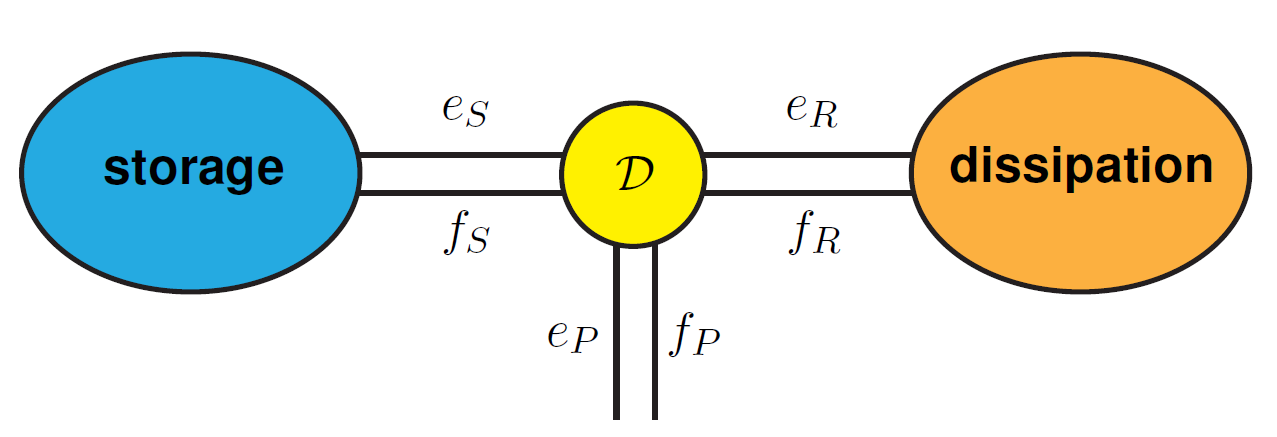
\includegraphics[width=0.55\textwidth]{diracstructure.png}
%	\caption[port-Hamiltonian system structure]{port-Hamiltonian system structure \cite{vanderSchaft_06}}
%	\label{FIG:pHsstructure}
%\end{figure}
\begin{figure}[b!]
	\centering
	\sf\small
	\def\svgwidth{0.6\columnwidth}
	\input{diracstructure.eps_tex}
	\caption{port-Hamiltonian system structure}
	\label{FIG:pHsstructure}
\end{figure}

Complex physical systems can be modelled as a network of energy storing and dissipating elements, similar to representation of electrical networks consisting of resistors, inductors and capacitors. The rules of interconnection are Newton's third law (action-reaction), Kirchhoff's laws and power-conserving elements like transformers or gyrators. The aim of PHS-modelling is to describe the power-conserving elements with the interconnection laws as a geometric structure and to define the Hamiltonian function as the total energy of the system. \\
The power flowing between the system's portions is described by the flow-effort product $e^Tf$. The external port $(f_P,e_P)$ describes the energy flow to/from environment or a controller. 

\subsection{Dirac structures and interconnection ports} \label{SS:PHSinterconnection}
The energy-routing structure forms the basis of every pHs. It can be compared to the printed circuit board in electronics, where capacitors, inductors and resistors are the energy-storing and damping elements. Mathematically it has the form of a \emph{Dirac} structure \cite{vanderSchaft_06}. The main property of a Dirac structure is power conservation, i.e. the power flowing into and out of it always sums to zero. We can define the set of ports $(f,e)$ connecting to the Dirac structure $\mathcal{D}$, thus 
\begin{equation}
e^Tf = 0 \;  \; \forall (f,e)\in\mathcal{D}
\end{equation}
Where $\mathcal{D}$ is a subspace of the space of flow and effort $\mathcal{D} \subset \mathcal{E}\times \mathcal{F}$. The space of flows is $f \in \mathcal{F}$ the space of efforts is its dual linear space $e \in \mathcal{E} = \mathcal{F}^*$. The Dirac structure has the same dimension than the space of flow $dim \mathcal{D} = dim \mathcal{F}$.
Further mathematical requirements can be found in literature \cite{vanderSchaft_06,Schaft_14}. The interconnection of ports is defined by the Dirac structure matrix $D$
\begin{equation}\
\begin{pmatrix}
e_P \\ f_S \\ e_R
\end{pmatrix} = D \begin{pmatrix}
f_P \\ e_S \\ e_R
\end{pmatrix}
\end{equation}
with the internal elements
\begin{equation}
D :=  \begin{pmatrix}
D_P & G_1 & G_2 \\ -G_1^T & D_S & G_3 \\ -G_2^T & -G_3^T & D_R 
\end{pmatrix}
\end{equation}
and $D_P,D_S,D_R$ are skew-symmetric, $G_*$ are arbitrary matrices. Thus $D = -D^T$ is skew-symmetric, which is necessary for $e^Tf=0$.
The power exchanged through a port is given by $ e_*^Tf_*$. In Fig. \ref{FIG:pHsstructure} the port variables entering the Dirac structure have already been split. 

\subsubsection{Energy storage port}
The port accounts for the internal storage of the system, its port variables are $ (f_S,e_S) $. The power supplied through this port is stored in the Hamiltonian energy function $H(x)$ of the system. Here $x$ denotes a general energy state variable. The resulting energy balance is:
\begin{equation}\label{EQ:storageport}
	\frac{d}{dt}H = \frac{\partial^T H}{\partial x}(x) \dot{x}
\end{equation}
The flow variable is the energy rate $ f_S = -\dot{x} $ and the effort variable is $ e_S = \frac{\partial H}{\partial x}(x) $.

\subsubsection{Energy dissipation port}
The port corresponds to internal dissipation and can be used to model resistive elements. The port variables are described by the general resistive relation
\begin{equation}
	F(f_R,e_R)=0
\end{equation}
with the property  $ e_R^T  f_R \leq 0 $ (energy dissipation). An important special case is the input-output resistive relation $f_R = -F(e_R)$, for linear elements simply
\begin{equation}
f_R = -Re_R \; , \; R=R^T\geq0
\end{equation}
For an uncontrolled system that does not interact with the environment, i.e. no energy exchange through the  external port, the energy balance is:
\begin{equation}
	\frac{dH}{dt} = -e_S^Tf_S = e_R^T f_R \leq 0
\end{equation}

\subsubsection{External port}
The external port $(f_P,e_P)$ can be further split into an environment \emph{interaction} $(f_I,e_I)$ and a \emph{control} port $(f_C,e_C)$, satisfying $e_P^Tf_P = e_I^Tf_I + e_C^Tf_C$.
The power balance of the whole system then is
\begin{equation}
	e_S^Tf_S + e_R^T f_R +e_I^Tf_I + e_C^T f_C = 0
\end{equation} 
or by using (\ref{EQ:storageport})
\begin{equation}\label{EQ:energybalance}
	\frac{dH}{dt} = e_R^T f_R +e_I^Tf_I + e_C^T f_C 
\end{equation}

\subsubsection{Interconnection of port-Hamiltonian systems}
It is important to notice that the interconnection of two pHs is again a pHs \cite{Schaft_14}. Consider two general pHs $(i=1,2)$ with open control and environment interaction ports:
\begin{eqnarray}
\begin{aligned}
	\dot{x}_i &= (J_i - R_i)\frac{\partial H_i}{\partial x_i}+ (g_i^C & g_i^I)\begin{pmatrix}f_i^C \\ f_i^I\end{pmatrix}\\
	\begin{pmatrix}e_i^C \\ e_i^I\end{pmatrix} &= \begin{pmatrix}(g_i^C)^T \\ (g_i^I)^T\end{pmatrix}\frac{\partial H_i}{\partial x_i}
\end{aligned}
\end{eqnarray}
where $J_i,R_i$ are a skew-symmetric structure matrix and a positive semi-definite symmetric dissipation matrix. $(g_i^C g_i^I)$ is a general input matrix respectively.
For notational convenience the usual dependencies on the states have been omitted. The control inputs and outputs are now connected by setting $f_1^C = e_2^C $ and $ f_2^C = -e_1^C $. Note that the minus sign is necessary for power conservation. The power exchanged by the $i$-th system is $P_i = (e_i^C)^Tf_i^C$, therefore the total exchanged energy fulfils $ P_1 + P_2 = 0 $. The resulting interconnected system has still the environment interaction ports open:
\begin{eqnarray}
\begin{aligned}
	\dot{x} &= (J - R)\frac{\partial H}{\partial x}+ (g_1^I & g_2^I)\begin{pmatrix}f_1^C \\ f_2^I\end{pmatrix}\\
	\begin{pmatrix}e_1^I \\ e_2^I\end{pmatrix} &= \begin{pmatrix}(g_1^I)^T \\ (g_2^I)^T\end{pmatrix}\frac{\partial H}{\partial x}
\end{aligned}
\end{eqnarray}
where $ x = (x_1, x_2)^T $ and $ H = H_1 + H_2 $ is the sum of the two energies. The structure and dissipation matrix become:
\[J = \begin{pmatrix} J_1 & g_1^C(g_2^C)^T \\ 
-g_2^C(g_1^C)^T & J_2\end{pmatrix} \, , \; 
R = \begin{pmatrix}
R_1 & 0 \\ 0 & R_2\end{pmatrix}\]



\section{3D-space modelling of mechanical systems}\label{S:3Dspace-modelling}


\subsection{Euclidean space and motions}\label{[SS:euclideanspacemotions]}
\subsubsection{Coordinate frames}
A coordinate frame of the three-dimensional Euclidean space is a 4-tuple of the form $ \Psi = (o,\hat{x},\hat{y},\hat{z})$. Where $ o $ is the three-dimensional vector of the origin and $ \hat{x},\hat{y},\hat{z} $ are the linear independent, orthonormal coordinate vectors. Consider two coordinate frames $ \Psi_1,\Psi_2 $ which share the same origin but differ in orientation due to different choices of $ \hat{x}_i,\hat{y}_i,\hat{z}_i, \; i=1,2 $. The change of orientation from $ \Psi_i $ to $ \Psi_j $ is described by the rotation matrix $ R_i^j $. The set of rotation matrices is called \emph{special orthonormal} group ($SO(3)$) \cite{Stramigioli_01b} and is defined as:
\begin{equation}
	SO(3) = \{R \in \mathbb{R}^{3 \times 3} \; | \; R^{-1} = R^T, det R = 1\}
\end{equation}
Usually coordinate frames are defined with respect to an inertial frame, and the coordinate vectors $ \hat{x},\hat{y},\hat{z} $ are chosen equal for all frames, deviations of orientation are represented by a rotation matrix relative to the inertial frame. In general a change of coordinate frames from $ \Psi_i $ to $ \Psi_j $ can be expressed with the homogeneous matrix
\[ H_i^j := \begin{pmatrix}R_i^j & p_i^j \\ 0_{1\times3} & 1\end{pmatrix} \]
where $p_i^j = o_j - o_i$ denotes the distance between the origins. A point $ p^i \in \mathbb{R}^3 $ expressed in $ \Psi_i $ is cast into $\Psi_j$ by
\begin{equation}\label{EQ:coordchange}
	\begin{pmatrix}p^j \\ 1\end{pmatrix} = H_i^j \begin{pmatrix}
		p^i \\ 1\end{pmatrix}
\end{equation}.
The inverse transformation $ H_j^i $ is given by 
\[H_i^j = (H_i^j)^{-1} = \begin{pmatrix}(R_i^j)^T & -(R_i^j)^T p_i^j \\ 0_{1 \times 3} & 1\end{pmatrix} \]
and is still a homogeneous matrix.
The set of homogeneous matrices is called the \emph{special Euclidean} group:
\begin{equation}
	SE(3) := \{\begin{pmatrix}R & p\\0 & 1\end{pmatrix} \; | \; R \in SO(3), p \in \mathbb{R}^3\} 
\end{equation}
The $SE(3)$ is a matrix Lie group, composed of the set of homogeneous matrices $H_i^j$ and the matrix multiplication being the group operation. For more information on Lie groups see e.g. \cite{Stramigioli_01}.
\subsubsection{Twists and wrenches}
Consider any point $ p $ not moving in coordinate frame $\Psi_i $, i.e. $ \dot{p}^i = 0 $. If $ p $ is moving in another coordinate frame $ \Psi_j $, the two frame move with respect to each other. The trajectory can be described as a function of time: $H_i^j(t) \in SE(3)$. By differentiating (\ref{EQ:coordchange}) one obtains
\[\begin{pmatrix}\dot{p}^j(t) \\ 1\end{pmatrix} = \dot{H}_i^j(t) \begin{pmatrix}p^i \\ 1\end{pmatrix} \]
$ \dot{H}_i^j $ describes both motion and a change of the reference frame. A separated representation is
\begin{equation}\label{EQ:twistrighttranslation}
	\begin{pmatrix}\dot{p}^j(t) \\ 1\end{pmatrix} = \tilde{T}_i^{j,j}\left(H_i^{j}\begin{pmatrix}p^i \\ 1\end{pmatrix}\right)
\end{equation}
$ \dot{H}_i^j$ is a tangential vector along the trajectory $H_i^j(t)$ and thus in the tangent space of the $SE(3)$: $ \dot{H}_i^j \in T_{H_i^j}SE(3)$. To obtain a representation of motion which is referenced to a coordinate frame, we can map $\dot{H}_i^j$ to the identity of the $SE(3)$. At the identity $ e $ of the $SE(3)$ the tangent space $ T_e SE(3) $ has the structure of a Lie algebra. The Lie algebra of the $SE(3)$ is denoted by $\mathfrak{se}(3)$. This is done either by left or right translation, for a definition see \cite{Stramigioli_01}. The right translation is used in (\ref{EQ:twistrighttranslation}) and is written compactly
\begin{equation}\label{EQ:righttranslation}
\dot{H}_i^j = \tilde{T}_i^{j,j} H_i^j
\end{equation}\label{EQ:lefttranslation}
The left translation leads to
\begin{equation}
\dot{H}_i^j = H_i^j \tilde{T}_i^{i,j} 
\end{equation}
We call $\tilde{T} \in T_e SE(3)$ a twist and the $\mathfrak{se}(3)$ the space of twists.
Let us look more closely at this representation by calculating the twist from the elements of the homogeneous matrix

\begin{eqnarray}\label{EQ:twistdecomposition}
\begin{aligned}
T_i^j &= \dot{H}_i^j H_j^i =
\begin{pmatrix}
\dot{R}_i^j & \dot{p}_i^j \\ 0 & 0
\end{pmatrix}
\begin{pmatrix}
R_j^i & p_j^i \\ 0 & 1
\end{pmatrix} = 
\begin{pmatrix}
\dot{R}_i^j & \dot{p}_i^j \\ 0 & 0
\end{pmatrix}
\begin{pmatrix}
(R_i^j)^T & -(R_i^j)^Tp_i^j \\ 0 & 1
\end{pmatrix} = \\ &= 
\begin{pmatrix}
\dot{R}_i^j(R_i^j)^T & -\dot{R}_i^j(R_i^j)^Tp_i^j + \dot{p}_i^j \\ 0 & 0
\end{pmatrix} =: 
\begin{pmatrix}
\tilde{\omega}_i^j & v_i^j \\ 0 & 0
\end{pmatrix}
\end{aligned}
\end{eqnarray}
It is clear from this equation that the linear velocity part $v_i^j$ is not the velocity of the frame $\Psi_i$ with respect to $\Psi_j$, identified by $\dot{p}_i^j$. This twist representation is described by the \emph{screw theory} (see e.g. \cite{KinematicsHandbook}). It can be visualized by the angular velocity around an axis and the linear velocity along this axis.



Next to the $4  \times 4$ matrix $\tilde{T} $ there exists also a vector representation $T\in \mathbb{R}^6$
\begin{equation}
 \tilde{T} = \begin{pmatrix}\tilde{\omega} & v \\ 0 & 0\end{pmatrix} \; , \; T = \begin{pmatrix}\omega \\ v\end{pmatrix} \end{equation}
wherein $v$ is the velocity and $\omega$ is the angular velocity. $\tilde{\omega}$ is the skew-symmetric representation of the vector $\omega$
\begin{equation}\label{EQ:skewsymmetricop}
\omega = \begin{pmatrix}
\omega_1 \\ \omega_2 \\ \omega_3\end{pmatrix} \; \Rightarrow \; \tilde{\omega} = \begin{pmatrix}0 & -\omega_3 & \omega_2 \\ \omega_3 & 0 & \omega_1 \\ -\omega_2 & \omega_1 & 0\end{pmatrix} \end{equation} \\

Left and right translations lead to different representations of a twist:
\begin{itemize}
\item $T_i^{k,j}$ is the twist of $\Psi_i$ with respect to $\Psi_j$ expressed in the frame $\Psi_k$
\item $T_i^j = T_i^{j,j}$ is the twist of $\Psi_i$ with respect to $\Psi_j$ expressed naturally in $\Psi_j$ 
\end{itemize}

Changes of coordinates for twists are of the form 
\begin{equation}
\tilde{T}_i^{j,j} = \tilde{T}_i^{j} = H_i^j \tilde{T}_i^{i,j} H_j^i\end{equation}
or for the vector representation
\begin{equation}
 T_i^{j} = Ad_{H_i^j} T_i^{i,j} \; , \;
Ad_{H_i^j} = \begin{pmatrix}R_i^j & 0 \\ \tilde{p}_i^j R_i^j & R_i^j\end{pmatrix} \end{equation}

The  dual vector space of $\mathfrak{se}(3)$ is the space of linear operations from $\mathfrak{se}(3)$ to $\mathbb{R} $. It is denoted by $\mathfrak{se}^*(3)$ and represents the space of wrenches $W$. Wrenches decompose to moments $ m $ and forces $ f $.
\begin{equation}
 W = ( m \;\; f) \; , \; \tilde{W} = \begin{pmatrix}
\tilde{m} & f \\ 0 & 0\end{pmatrix} \end{equation}
Again $\tilde{W} \in \mathbb{R}^{4\times 4}$ is a matrix while $W \in \mathbb{R}^6$ is the  row vector representation.
The change of coordinates for twists is similar to the case of twists:
\begin{equation}
(W_i^{k,i})^T = Ad_{H_k^i}^T (W_i^i)^T \end{equation} 
Here the mapping is in the opposite direction, from $\Psi_j$ to $\Psi_i$, what is a consequence of the fact that wrenches are duals to twists. Again there are different representations of wrenches: \begin{itemize}
\item $W_i^{k,j}$ is the wrench applied to a spring connecting $\Psi_i$ to $\Psi_j$ on the side of $\Psi_i$ expressed in the coordinate frame $\Psi_k$.
\item $W_i^k $ is the wrench applied to a body attached to $\Psi_i$ expressed in the coordinate frame $\Psi_k$.
\end{itemize}
These definitions lead to the following rules of interconnection:
Connecting a body and spring in the point $\Psi_i$ and applying the principle of action and reaction we get $W_i^{k,j} = -W_i^k$. Due to the nodicity of a spring we have $ W_i^{k,j} = -W_j^{k,i} $\\

We define power flowing through a port by the duality product of flow and effort, in the mechanical domain this twist and wrench. On a vector space level the power port $\mathcal{P}$ is defined by the Cartesian product of the Lie algebra $\mathfrak{se}(3)$ and its dual $\mathfrak{se}^*(3)$: $\mathcal{P} = \mathfrak{se}(3) \times \mathfrak{se}^*(3)$.

\subsubsection{General input-state-output port-Hamiltonian systems}
The simple relation $\dot{q}=\frac{\partial H}{\partial p}$ does not hold for a 3D-mechanical system. With reference to the next section we find $\frac{\partial V}{\partial P_i^i} = T_i^{i,0} = H_0^i \dot{H_i^0}$, with the $H_0^i$ being the configuration variable and $P_i^i$ the momentum. For reasons of notational clarity the Hamiltonian is denoted with $V$. The interconnecting Dirac structure in 3D-mechanical system  is dependent on the configuration and we call it a \emph{modulated} Dirac structure. This motivates the more general concept of port-Hamiltonian systems on \emph{manifolds}. By introducing local coordinates $x$ on the state manifold $\mathcal{X}$, we can associate the flows towards the energy storage with $f_s = -\dot{x}$ and the efforts with $e_s = \frac{\partial V}{\partial x}$. The flows are elements of the tangent space of the state manifold $T_x\mathcal{X}$ and the efforts are elements of the co-tangent space $T_x^*\mathcal{X}$. A general port-Hamiltonian system defined on $\mathcal{X}$ is of the form
\begin{eqnarray}
\begin{aligned}
\dot{x} &= [J(x)-R(x)]\frac{\partial V}{\partial x}(x) + g(x) u \\
y &= g^T(x)\frac{\partial V}{\partial x}
\end{aligned}
\end{eqnarray}
with a skew-symmetric matrix $J(x)$ and a resistive structure matrix $R(x)$ which is symmetric and positive semi-definite. Clearly $u$ and $y$ denote the input and output respectively and we call this representation \emph{input-state-output} form \cite{Schaft_14}. In the following section we introduce the corresponding representations of atomic mechanical elements.




\subsection{Dynamics of physical components}
\subsubsection{Springs}
A \emph{spring} is the ideal, lossless element storing potential energy. It is connected to two bodies and is defined by a potential energy function. The energy is a function of the relative displacement of the attached bodies. Consider a spring between the two bodies $ B_i $ and $ B_j $,  with coordinate frames $ \Psi_i $ and $ \Psi_j $ fixed to the respective body. The stored potential energy is positive definite function $V_{i,j}$ of the form 
\begin{equation}
	V_{i,j} : SE(3) \rightarrow \mathbb{R}; \; H_i^j \mapsto V_{i,j}(H_i^j)
\end{equation}
For explicit energy functions for different types of springs see \cite{Stramigioli_01b}.
The input-state-output form is defined by the relative displacement $H_i^j$ (state variable), the wrench $W_i^{j,j}$ (effort) and the twist $T_i^j$ (flow).
\begin{eqnarray}
\begin{aligned}
	&\dot{H}_i^j = T_i^{j}H_i^j\\
	&W_i^{j,j} = \frac{\partial V_{i,j}}{\partial H_i^j}(H_i^j)^T
\end{aligned}
\end{eqnarray}
Note that $ V_{i,j} $ is an energetic minimum when $ H_i^j $ is the identity matrix $I_4$. An energetic minimum is physically necessary, otherwise infinite energy would be extractable from the spring. With $ H_i^j = I_4 $ the frames $ \Psi_i $ and $\Psi_j$ coincide.
It is possible to define springs with non-zero rest-length by introducing coordinate frames $ \Psi_{ic} $ and $\Psi_{jc}$ rigidly attached to $ \Psi_i $ and $\Psi_j$ respectively. The spring is now between the new frames, thus the energetic minimum is $H_{ic}^{jc} = I_4$. The displacements $ H_i^{ic}, H_j^{jc} $ are the resulting rest-lengths. Frames $ \Psi_{ic} $ and $\Psi_{jc}$ can be chosen to represent the \emph{center of stiffness}, where translation and rotation are maximally decoupled \cite{Stramigioli_99}.


\begin{comment}
\subsubsection{Variable rest-length springs}
Varying the rest-lengths of springs in manipulator-object interaction allows to perform a grasp and specify grasping forces. The rest-length influences the energy configuration, to allow for controlled changes of rest-length an additional power port is introduced. The chosen hinge points $ \Psi_b,\Psi_j $ of the spring define an axis, known as the principal axes of stiffness. Changes of the rest-length leave this axis unaffected, i.e. the displacement is in-line. With reference to Fig. \ref{FIG:variablespring}, the change of rest-length is a change of relative displacement of $ \Psi_b $ and $\Psi_i$: $H_i^b$.
\begin{figure}[htb]
	\centering
	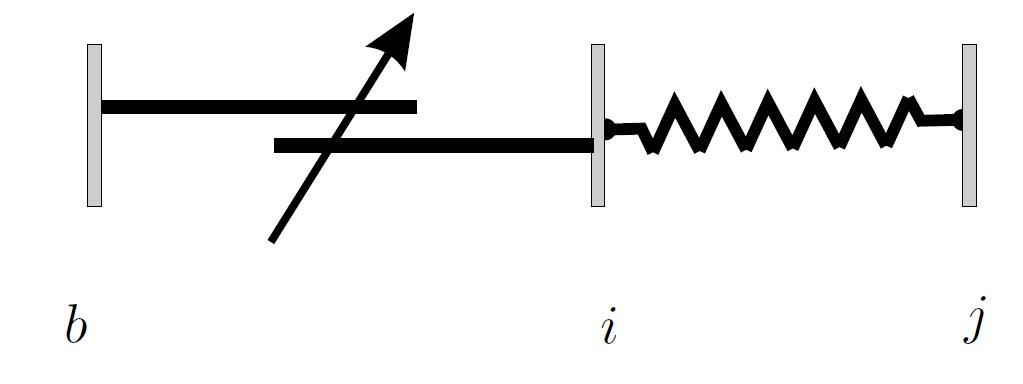
\includegraphics[width=0.55\textwidth]{variablespring.jpg}
	\caption[Variable rest-length spring]{Variable rest-length spring \cite{Stramigioli_99}}
	\label{FIG:variablespring}
\end{figure}
Towards a PHS representation we need to identify the components contributing to the deformation twist of the spring $ T_i^{j} $: the displacement twist of the bodies attached to the spring $T_b^{j} $ and the twist resulting from a commanded change of the rest-length $T_i^{b}$ \cite{Stramigioli_01c}.
\begin{equation}
	T_i^{j} = T_b^{j} + Ad_{H_b^j} T_i^{b}
\end{equation}
Since no additional energy storages were introduced, the Hamiltonian function is equal to the case of the simple spring. We can write the two-port Hamiltonian system of a variable length spring as
\begin{eqnarray}\label{EQ:variablerestlengthspring}
\begin{aligned}
	&\dot{H}_i^j =\left( \begin{pmatrix}1 & Ad_{H_b^j}\end{pmatrix} \begin{pmatrix}T_b^{j} \\ T_i^{b}\end{pmatrix} \right) H_i^j\\
	&\begin{pmatrix}W_b^{j,j} \\ W_i^{b,b}\end{pmatrix}  = \left( \begin{pmatrix}1 \\ Ad_{H_b^j}^T\end{pmatrix} \frac{\partial V_{i,j}}{\partial H_i^j} \right) (H_i^j)^T
\end{aligned}
\end{eqnarray}
\end{comment}

\subsubsection{Inertias}
Inertias are special since they in general store two types of energy: kinetic and potential energy due to gravitation. At first we exclude the gravitational terms and focus on motion. Kinetic energy is a function of the relative motion w.r.t. an inertial reference. When expressing motion in non-inertial or accelerated reference frames, fictitious forces such as the \emph{Coriolis} or the \emph{centrifugal} force need to be considered.\\
Let us start from \emph{Newton's} second law of dynamics, the time derivative of a body's momentum is equal to the applied wrench.
\begin{equation}
\dot{P}_b^0 = W_b^0
\end{equation}
The momentum of the inertia $b$ and the wrench acting on it are both expressed in the inertial reference frame $\Psi_0$. Let us consider the non-inertial frame $\Psi_b$, fixed to the inertia. We start by changing coordinates, clearly we have $W_b^0 = Ad_{H_0^b}^T W_b^b$. It is detailed in \cite{Stramigioli_01} that $P_0^b \in \mathfrak{se}^*(3)$ and thus the same transformation as for wrenches applies $P_b^0 = Ad_{H_0^b}^T P_b^b$. Expressing the \emph{Newton's} second law in the non-inertial frame $\Psi_b$ we have
\begin{equation}
\frac{d}{dt}(Ad_{H_0^b}^T P_b^b) = Ad_{H_0^b}^T W_b^b
\end{equation}
The evolution of the accelerated body frame $\Psi_b$ w.r.t to the inertial frame is time dependent. The time derivative of the transformation is $\frac{d}{dt}Ad_{H_0^b}^T = -Ad_{H_0^b}^T ad_{T_b^{b,0}}^T $, with the \emph{adjoint} representation (see for example \cite{Stramigioli_01b}):
\begin{equation}\label{EQ:adjointmapping}
ad_{T_b^{b,0}}^T = \begin{pmatrix}
-\tilde{\omega}_b^{b,0} & -\tilde{v}_b^{b,0} \\ 0 & -\tilde{\omega}_b^{b,0}\end{pmatrix}
\end{equation}
The second law of dynamics expressed in the body's frame is then
\begin{eqnarray}
\begin{aligned}
Ad_{H_0^b}^T \dot{P}_b^b -Ad_{H_0^b}^T ad_{T_b^{b,0}}^T P_b^b &= Ad_{H_0^b}^T W_b^b \\
\dot{P_b^b} &= ad_{T_b^{b,0}}^T P_b^b + W_b^b
\end{aligned} 
\end{eqnarray}
This formulation is split into its rotational and translational components, then we can exchange twist and momentum by the following operation
\begin{equation}\label{EQ:centripetaldetail}
\begin{pmatrix}
\dot{P}_{b,\omega}^b \\ \dot{P}_{b,v}^b \end{pmatrix} = \begin{pmatrix}
-\tilde{\omega}_b^{b,0} & -\tilde{v}_b^{b,0} \\ 0 & -\tilde{\omega}_b^{b,0}\end{pmatrix} \begin{pmatrix}
P_{b,\omega}^b \\ P_{b,v}^b 
\end{pmatrix} + W_b^b = \begin{pmatrix}
\tilde{P}_{b,\omega}^b & \tilde{P}_{b,v}^b \\ \tilde{P}_{b,v}^b & 0
\end{pmatrix} \begin{pmatrix}
\omega_b^{b,0} \\ v_b^{b,0}
\end{pmatrix} +W_b^b
\end{equation}
This clearly corresponds to the classical description of a rigid body's dynamics of the form
\begin{equation}
	\dot{P}_b^b = M_b \dot{T}_b^{b,0}  = C_b T_b^{b,0} + W_{b}^b
\end{equation}
Here $M_b$ describes the body's inertia and $C_b$ accounts for Coriolis and centrifugal terms.\\
Towards port-Hamiltonian representation we start from the kinetic (co-)energy given by $V_k^*(T_b^{b,0}) =\frac{1}{2}(T_b^{b,0})^T M_b T_b^{b,0}$. Formally speaking the kinetic energy is a function of the momentum. By using the relation of twist and momentum $P_b^b = M_b T_b^{b,0}$ we get the kinetic energy
\begin{equation}
V_k(P_b^b) = \frac{1}{2}(P_b^b)^T M_b^{-1} P_b^b
\end{equation}
By differentiating the kinetic energy w.r.t to the state variable $P_b^b$ we obtain 
\begin{equation}
\frac{\partial V_k(P_b^b)}{\partial P_b^b} = M_b^{-1} P_b^b = T_b^{b,0}
\end{equation}
Recall from Table \ref{TAB:PHSvar_mechanic} that the twist is the effort variable in the port-Hamiltonian representation of an inertia. The flow is the externally supplied wrench $W_b^b$, thus we obtain the port-Hamiltonian representation of a rigid body, neglecting gravity
\begin{eqnarray}\label{EQ:PHSsimpleinertia}
\begin{aligned}
	&\dot{P_b^b} = C_b \frac{\partial V_k(P_b^b)}{\partial P_b^b} + I_6 W_{b}^b \\
	&T_b^{b,0} = I_6 \frac{\partial V_k(P_b^b)}{\partial P_b^b}
\end{aligned}
\end{eqnarray}
In cooperative manipulation we often deal with heavy objects, it is thus inevitable to include the potential energy resulting from the gravitational field. One can think of a spring connecting the body and an inertial frame associated with the ground. This spring can be formulated as a pHs using the left translation (\ref{EQ:lefttranslation})
\begin{eqnarray}\label{EQ:gravityspring}
\begin{aligned}
	&\dot{H}_b^0 = H_b^0 T_b^{b,0}\\
	&W_b^{b,0} = (H_b^0)^T\frac{\partial V_{g}}{\partial H_b^0}
\end{aligned}
\end{eqnarray}
Where $V_g$ is a suitable energy function. For a combined description the potential and kinetic energy add up: $V_{kg} = V_k + V_g$. Since there are two types of energy stored by \emph{one} body, the twists in both energy systems are equal. The wrenches on the body add up   
\[W_{kg}^b = W_{b}^b + C_b \frac{\partial V_{kg}}{\partial P_b^b} - (H_b^0)^T \frac{\partial V_{kg}}{\partial H_b^0} \]
Note that the negative sign in the upper equation comes from $W_b^b = - W_b^{b,0} $.\\
With this knowledge we can write the combined PHS representation
\begin{eqnarray} \label{EQ:PHSinertia}
\begin{aligned}
&\begin{pmatrix}\dot{H}_b^0 \\ \dot{P_b^b}\end{pmatrix} =
\begin{pmatrix} 0 & H_b^0  \\
- (H_b^0)^T & C_b\end{pmatrix}
\begin{pmatrix}\frac{\partial V_{kg}}{\partial H_b^0} \\ \frac{\partial V_{kg}}{\partial P_b^b}\end{pmatrix}+
\begin{pmatrix}0 \\ I_6\end{pmatrix} W_{b}^b \\
&T_b^{b,0} = \begin{pmatrix}0 & I_6\end{pmatrix}
\begin{pmatrix}\frac{\partial V_{kg}}{\partial H_b^0} \\ \frac{\partial V_{kg}}{\partial P_b^b}\end{pmatrix}
\end{aligned}
\end{eqnarray}


\subsubsection{Dampers}\label{SSS:Dampers}
Dampers do not have a state since they do not store energy, they only dissipate it. Note that energy is not "destroyed" in the dampers but transformed into thermal energy. This can be modelled with a thermal port connected to the environment, for reasons of simplicity we discard the generated thermal energy. The easiest way to achieve damping is a linear resistive element $R$, such that the wrench is directly proportional to twist. Consider for example a body's motion with respect to the inertial frame
\begin{equation}
	W_b^b = R T_b^{b,0}
\end{equation}
Or a damper in parallel with spring
\begin{equation}
	W_i^{j,j} = R T_i^{j}
\end{equation}
The dissipated co-energy is $E_d = \frac{1}{2}T^T R T$.


\section{Spring-mass-damper systems}\label{S:springmassdampers}
Recall the motivating example from Section \ref{S:HSdescription} of a simple spring-mass system. We can add a damper $d$ to the port-Hamiltonian representation and rewrite eq. (\ref{EQ:HSexample})
\begin{equation}
	\begin{pmatrix}\dot{q} \\ \dot{p}\end{pmatrix} =
	\begin{pmatrix}0 & 1 \\ -1 & -d\end{pmatrix}
	\begin{pmatrix}\frac{\partial V}{\partial q}(q,p) \\ \frac{\partial V}{\partial p}(q,p)\end{pmatrix} + 
	\begin{pmatrix}0 \\ 1\end{pmatrix} F_e\\  
\end{equation}
Clearly $\dot{p} = -\frac{\partial V}{\partial q}(q,p)-d\frac{\partial V}{\partial p}(q,p)+F_e$ equals the mechanical impedance relation $m\ddot{x} + d\dot{x} +kx = F_e$. Thus we have a port-Hamiltonian representation of the impedance control scheme. This is the basis for the control architecture presented below. Therefore the mass-spring-damper system, given as a one-dimensional example, is formulated in the $SE(3)$. We start from eqs. (\ref{EQ:PHSsimpleinertia},\ref{EQ:gravityspring}) and add another spring to the body associated with $\Psi_b$. This spring connects to a desired object position assigned to $\Psi_v$. Its port-Hamiltonian representation is given by
\begin{eqnarray}
\begin{aligned}
	&\dot{H}_b^v = H_b^v T_b^{b,v}\\
	&W_b^{b,v} = (H_b^v)^T\frac{\partial V_{s}}{\partial H_b^v}
\end{aligned}
\end{eqnarray}
The spring's deformation twist is decomposed by $T_b^{b,v} = T_b^{b,0} - T_v^{b,0}$.
The damping along this spring is $W_b^b = D_b T_b^{b,v} $. Body, spring and damper move uniformly with the twist $T_b^{b,0}$ and the wrenches add up. Combing all components we arrive at
\begin{eqnarray} \label{EQ:externalimpedance}
\begin{aligned}
&\begin{pmatrix}\dot{H}_b^0 \\ \dot{H}_b^v \\  \dot{P_b^b}\end{pmatrix} =
\begin{pmatrix} 0 & 0 & H_b^0  \\ 0 & 0 & H_b^v \\
- (H_b^0)^T & -(H_b^v)^T & C_b-D_b\end{pmatrix}
\begin{pmatrix}\frac{\partial V_{kgs}}{\partial H_b^0}\\ \frac{\partial V_{kgs}}{\partial H_b^v} \\ \frac{\partial V_{kgs}}{\partial P_b^b}\end{pmatrix}+
\begin{pmatrix} 0 & 0\\ -H_b^v Ad_{H_0^b} & 0 \\ D_b Ad_{H_0^b} & I_6 \end{pmatrix}\begin{pmatrix} T_v^0 \\ W_{b}^b\end{pmatrix} \\
&\begin{pmatrix}W_v^{0,0} \\ T_b^{b,0}\end{pmatrix} = \begin{pmatrix}0 & -Ad_{H_0^b}^T (H_b^v)^T & Ad_{H_0^b}^T D_b\\ 0 & 0 & I_6 \end{pmatrix}
\begin{pmatrix}\frac{\partial V_{kgs}}{\partial H_b^0}\\ \frac{\partial V_{kgs}}{\partial H_b^v} \\ \frac{\partial V_{kgs}}{\partial P_b^b}\end{pmatrix}
\end{aligned}
\end{eqnarray}
In a cooperative manipulation set-up this clearly accounts for an \emph{external} impedance relation, used to establish compliant behaviour between (virtual) object and environment. Analogously we can define impedance relations between manipulators and virtual object. To this purpose we define a manipulator inertia and connect to the object with a spring and a damper. Here we consider the manipulator masses to be gravity pre-compensated and omit the spring connecting to the ground. The $i$-th manipulator inertia is given by
\begin{eqnarray}
\begin{aligned}
	&\dot{P_i^i} = C_i \frac{\partial V_{k(i)}(P_i^i)}{\partial P_i^i} + I_6 W_{i}^i \\
	&T_i^{i,0} = I_6 \frac{\partial V_{k(i)}(P_i^i)}{\partial P_i^i}
\end{aligned}
\end{eqnarray}
It is important that the spring connecting $b$ and $i$ does not connect to the center of the object $b$ but to a point $b(i)$ on the surface of $b$. Clearly the distance $p_{b(i)}^b$ corresponds to the extent of the object. The spring's twist decomposes as follows
\begin{equation}
T_{b(i)}^i = T_b^i + T_{b(i)}^{i,b} = Ad_{H_b^i} T_b^{b,0} - T_i^{i,0} + Ad_{H_b^i}\underbrace{T_{b(i)}^b}_{=0}
\end{equation}
The spring is given by    
\begin{eqnarray}
\begin{aligned}
&\dot{H}_{b(i)}^i = H_{b(i)}^i \begin{pmatrix}
Ad_{H_b^{b(i)}} & - Ad_{H_i^{b(i)}} \end{pmatrix} \begin{pmatrix} 
T_b^{b,0} \\ T_i^{i,0}\end{pmatrix}\\
&\begin{pmatrix} 
W_b^{b,0} \\ W_i^{i,0} \end{pmatrix} = \begin{pmatrix}
Ad_{H_b^{b(i)}}^T \\ - Ad_{H_i^{b(i)}}^T\end{pmatrix}
(H_{b(i)}^i)^T
\frac{\partial V_{s(i)}}{\partial H_{b(i)}^i}
\end{aligned}
\end{eqnarray}
and the damper along the spring exerts a wrench on the body $i$
\begin{equation}
W_i^i = D_i T_i^{i,b} = D_i T_i^{i,0} - D_i Ad_{H_b^i} T_b^{b,0}.
\end{equation}
We can combine spring, inertia and damper, the twist $T_i^{i,0}$ is the common quantity.
\begin{eqnarray}\label{EQ:internalimpedance}
\begin{aligned}
\begin{pmatrix}\dot{H}_{b(i)}^i \\ 
\dot{P_i^i} \end{pmatrix} &= \begin{pmatrix}
0 & -H_{b(i)}^i Ad_{H_i^{b(i)}} \\
Ad_{H_i^{b(i)}}^T (H_{b(i)}^i)^T & C_i - D_i
\end{pmatrix}
\begin{pmatrix}
\frac{\partial V_{ks(i)}}{\partial H_{b(i)}^i} \\ 
\frac{\partial V_{ks(i)}}{\partial P_{i}^i}
\end{pmatrix} + \\ &+
\begin{pmatrix}
H_{b(i)}^i Ad_{H_b^{b(i)}} & 0 \\
D_i Ad_{H_b^i} & I_6
\end{pmatrix}
\begin{pmatrix}
T_b^{b,0} \\ W_i^i
\end{pmatrix}
 \\
\begin{pmatrix}
W_b^{b,0} \\ T_i^{i,0}
\end{pmatrix} &= 
\begin{pmatrix}
Ad_{H_b^{b(i)}}^T (H_{b(i)}^i)^T &  Ad_{H_b^i}^T D_i^T \\
 0 & I_6
\end{pmatrix}
\begin{pmatrix}
\frac{\partial V_{ks(i)}}{\partial H_{b(i)}^i} \\ 
\frac{\partial V_{ks(i)}}{\partial P_{i}^i}
\end{pmatrix}
\end{aligned}
\end{eqnarray}


\section{Imposing constraints}\label{S:ImposingConstraints}
The interconnection of a spring and an inertia is the the ideal pair in terms of input-output causality. The spring expects a twist-input and outputs a wrench. The inertia has a wrench-input and outputs a twist. It can be seen from eq. (\ref{EQ:PHSinertia}) that the interconnection of inertia and spring gives a set of ordinary differential equations (ODE). Many mechanical systems cannot be modelled by an interconnection of springs and masses. The prime example is the contact of two rigid objects, rigid means there is no elastic deformation which could be modelled by a spring (for an extensive treatment of hard and soft contact see \cite{Duindam_09}). Rigidly connected objects cannot move with respect to each other, i.e. they move with the same velocity. In cooperative manipulation we often assume the manipulators rigidly connected to the common object. The attempt to  move the bodies individually results in \emph{internal} forces. We call a force internal if it produces no \emph{virtual work} with the system's velocity (see \cite{Erhart_16} for a formal definition). The motion-limiting conditions are called kinematic \emph{constraints} and are expressed in the form
\begin{equation}
A^T(q)\dot{q}=0
\end{equation}
We call $A(q)$ the \emph{constraint} matrix and start from the Euler-Lagrange equations of constrained motion \cite{duindam2009geoplexbook}
\begin{eqnarray}
\begin{aligned}
\frac{d}{dt}\left(\dfrac{\partial \mathcal{L}}{\dot{q}}\right) - \frac{\partial \mathcal{L}}{\partial q} &= g(q)f + A(q)\lambda
\\
A^T(q)\dot{q} &= 0
\end{aligned}
\end{eqnarray}
The associated constraint forces are given by $A(q)\lambda$, where we call $\lambda$ the \emph{Lagrange} multipliers. They are uniquely determined if the constraints are satisfied, i.e. are given by the requirement $A^T(q)\dot{q}=0$. In this case the constraint forces do not influence the energy of the system since $\lambda^T (A^T(q)\dot{q}) = 0$, this corresponds to the requirement of a zero virtual work for internal forces. Similarly to Section \ref{S:HSdescription}, the Euler-Lagrange equations can be transformed to a port-Hamiltonian equivalent, which is a mixed set of differential and algebraic equations (DAE).
\begin{eqnarray}\label{EQ:PHSpconstrained}
\begin{aligned}
\begin{pmatrix}
\dot{q} \\ \dot{p} \end{pmatrix} &= 
\begin{pmatrix} 0 & I \\ -I & 0\end{pmatrix}
\begin{pmatrix}
\frac{\partial V}{\partial q} \\ \frac{\partial V}{\partial p}\end{pmatrix}
+ \begin{pmatrix}0 & 0 \\ A(q) & g(q)\end{pmatrix}
\begin{pmatrix}\lambda \\ f\end{pmatrix}
\\
\begin{pmatrix}0 \\ e\end{pmatrix} &=
\begin{pmatrix}0 & A^T(q) \\ 0 & g^T(q)\end{pmatrix}
\begin{pmatrix}
\frac{\partial V}{\partial p} \\ \frac{\partial V}{\partial p}\end{pmatrix}
\end{aligned}
\end{eqnarray}
The system is no longer described in the input-state-output form, but in an implicit form. Several approaches to solve the algebraic equations and restore the desired input-state-output form exist. Most of them are designed for generalized configuration $q$ and momentum $p$ coordinates, see e.g. \cite{Schaft_13},\cite{Duindam_09}. Due to non-linearity of $\dot{q}=\frac{\partial V}{\partial p}$ in mechanical systems not all are feasible for six dimensional systems. \\
The following method (described e.g. in \cite{Duindam_09}) uses the time-derivative of the constraints
\begin{equation}\label{EQ:constraintderivative}
0 = \frac{d}{dt}\left(A^T(q)\frac{\partial V}{\partial p}\right)
\end{equation}
We use the property $\frac{\partial V}{\partial p}=M^{-1}p$ for an energy function of the form $V = \frac{1}{2}p^TM^{-1}p + V_q$. Since $q(t)$ is time-dependent \emph{indirect dependencies} arise in $A(q),p(q)$ when calculating the total time-derivative
\begin{eqnarray}
\begin{aligned}
0 &= \frac{d}{dt}(A^TM^{-1}p) = \frac{\partial (A^TM^{-1}p)}{\partial q}\dot{q} + A^TM^{-1}\dot{p} = \\ &= \frac{\partial (A^TM^{-1}p)}{\partial q}M^{-1}p + A^TM^{-1}\left(-\frac{\partial V}{\partial q}+A(q)\lambda +g(q)f\right)
\end{aligned}
\end{eqnarray}
Solving this equation for $\lambda$ gives an analytic expression for the constrained forces
\begin{equation}
\lambda = (A^T M^{-1} A)^{-1} \left(-\frac{\partial (A^TM^{-1}p)}{\partial q}M^{-1}p + \frac{\partial V}{\partial q} - gf\right)
\end{equation}
Then $\lambda$ is re-inserted into eq. (\ref{EQ:PHSpconstrained}) and we obtain a set of ODEs in input-output form. Clearly the term $A(q)\lambda$ generates compensation forces that oppose relative motions of the bodies and keep the constraints $A^T(q)\dot{q}$ fulfilled. Since we computed the constraint forces starting from the time-derivative of the constraint, $A^T(q)\dot{q}$ stays constant. To guarantee $A^T(q)\dot{q}=0$, this must be already fulfilled in the beginning.
%Another approach is to find new coordinates for the momentum that limit the \emph{phase space} $(q,p)$ to motions fulfilling the constraints. Therefore we introduce the transformation
%\begin{equation}
%p = S(q)\bar{p}
%\end{equation}
%The definition of $S(q)$ is directly given by the constraint 
%\begin{equation}
%0 = A^T(q) M^{-1} p = A^T(q) M^{-1} S(q) \bar{p}
%\end{equation}
%S(q) is thus the \emph{kernel} of $A^T(q) M^{-1}$. The transformation is energy-conservative i.e.
%\begin{equation}
%\bar{V}(q,\bar{p}) := \frac{1}{2}\bar{p}^T\bar{M}^{-1}\bar{p} + V_q = \frac{1}{2}p^TM^{-1}p + V_q = V(q,p)
%\end{equation}
%Thus the constrained inertia matrix is $\bar{M} = (S^TM^{-1}S)^{-1}$.   
%We start re-writing eq. (\ref{EQ:PHSpconstrained}) using $p = S(q)\bar{p}$ and obtain
%\begin{eqnarray}
%\begin{aligned}
%\dot{q} &= \frac{\partial V}{\partial p} = M^{-1}p = M^{-1}S\bar{p} = M^{-1}S\bar{M}\bar{M}^{-1}\bar{p} = M^{-1}S\bar{M}\frac{\partial \bar{V}}{\partial \bar{p}}\\
%\dot{p} &= \frac{d}{dt}(S(q)\bar{p}) = \frac{\partial(S\bar{p})}{\partial q} \dot{q} +S\dot{\bar{p}} = -\frac{\partial V}{\partial q} + A\lambda + gf
%\end{aligned}
%\end{eqnarray}
%Towards a standard port-Hamiltonian representation we are seeking to express the last equation in the form $\dot{\bar{p}} = ...$. Therefore the equation is pre-multiplied with $\bar{M}S^TM^{-1}$
%\begin{eqnarray}\label{EQ:PHSconstrainedpremult}
%\begin{aligned}
%\bar{M}S^TM^{-1}\frac{\partial(S\bar{p})}{\partial q} \dot{q} + \bar{M}\underbrace{S^TM^{-1}S}_{\bar{M}^{-1}}\dot{\bar{p}} = \bar{M}S^TM^{-1}\left(-\frac{\partial V}{\partial q} + A\lambda + gf\right)
%\end{aligned}
%\end{eqnarray}
%For a symmetric $M$ we have $(S^TM^{-1}A)^T = A^T(q) M^{-1} S(q) = 0$. Since $S(q)$ is dependent on $q$ we need to consider indirect dependencies when differentiating 
%\begin{equation}
%\frac{\partial \bar{V}}{\partial q} = \frac{\partial V}{\partial q} + \frac{\partial^T (S(q) \bar{p})}{\partial q}\dot{q} = \frac{\partial V}{\partial q} + \frac{\partial^T (S(q) \bar{p})}{\partial q}M^{-1}S\bar{M}\frac{\partial \bar{V}}{\partial \bar{p}}
%\end{equation}
%Inserting this into eq. (\ref{EQ:PHSconstrainedpremult}) and re-arranging we desired port-Hamiltonian representation
%\begin{eqnarray}
%\begin{aligned}
%\begin{pmatrix}
%\dot{q} \\ \dot{\bar{p}}
%\end{pmatrix} &= 
%\begin{pmatrix}
%0 & M^{-1}S\bar{M} \\
%\bar{M}S^TM^{-1} & \bar{M}S^TM^{-1}\left(\frac{\partial^T (S(q) \bar{p})}{\partial q} - \frac{\partial (S(q) \bar{p})}{\partial q}\right)M^{-1}S\bar{M}
%\end{pmatrix}
%\begin{pmatrix}
%\frac{\partial \bar{V}}{\partial q} \\
%\frac{\partial \bar{V}}{\partial \bar{p}}
%\end{pmatrix} + \\
%&+ 
%\begin{pmatrix}
%0 \\ \bar{M}S^TM^{-1}
%\end{pmatrix}f
%\end{aligned}
%\end{eqnarray}
%Conclusively we have obtained two different representations of constrained systems in input-output form. The first one allows explicitly to calculate the constraint forces necessary to comply with the constraints. The second one restricts the possible motion and results in a system of reduced \emph{degrees of freedom}. We see in the remainder that the first can be exploited for control issues. 


\subsubsection{Constraints for 6D-motion}  


Consider two rigidly connected bodies, associated with the frames $\Psi_b$ and $\Psi_i$ and a distance between them $p_i^b = p_i^0 - p_b^0$. Clearly, in the setting of cooperative manipulation, one can think of an object $b$ and the $i$-th manipulator attached to it. Now let the body $b$ rotate with the angular velocity $\omega_b^0$. Being rigidly attached the body $i$ rotates in the same manner, $\omega_i^0 = \omega_b^0$. The translational velocity of body $i$ is expressed dependent on body $b$ by 
\begin{eqnarray}
\begin{aligned}
&\dot{p}_i^0 = \dot{p}_b^0 + \omega_b^0 \times p_i^b = \dot{p}_b^0 + \omega_b^0 \times (p_i^0-p_b^0) \\
&\dot{p}_i^0 - \omega_b^0 \times p_i^0 = \dot{p}_b^0 - \omega_b^0 \times p_b^0 \\
\end{aligned}
\end{eqnarray}
Recall the definition of the linear velocity component of a twist from eq. (\ref{EQ:twistdecomposition}) being $v_i^j= \dot{p}_i^j - \omega_i^j \times p_i^j$. Thus we have $v_i^0 = v_b^0$ and consequently $T_i^0 = T_b^0$. For a system of $i=1...N$ manipulators we write the constraints
\begin{equation}
0 = A^T T = \begin{pmatrix}
-I_3 & 0_3 & I_3 & 0_3 & & & \\
0_3 & -I_3 & 0_3 & I_3 & & & \\
\vdots & \vdots & & & \ddots & & & \\
- I_3 & 0_3 & & & & I_3 & 0_3 \\
0_3 & -I_3 & & & & 0_3 & I_3 
\end{pmatrix}
\begin{pmatrix}
T_b^0 \\ T_1^0 \\ \vdots \\ T_N^0
\end{pmatrix}
\end{equation}
We start by differentiating the constraints, here $A$ is not time or configuration dependent, thus $0=A^T\dot{T}$. Consider the simple example of two rigidly connected bodies $b$ and $i$, the constraint equation is
\begin{eqnarray}
\begin{aligned}
0 &= \dot{T}_i^0 - \dot{T}_b^0 = \begin{pmatrix}
\dot{\omega}_i^0 - \dot{\omega}_b^0 \\ \dot{v}_i^0 - \dot{v}_b^0
\end{pmatrix} =
\begin{pmatrix}
\dot{\omega}_i^0 - \dot{\omega}_b^0 \\ \frac{d}{dt}(\dot{p}_i^0 - \omega_b^0 \times p_i^0) - \frac{d}{dt}(\dot{p}_b^0 - \omega_b^0 \times p_b^0)
\end{pmatrix}= 
%\\ &=
%\begin{pmatrix}
%\dot{\omega}_i^0 - \dot{\omega}_b^0 \\
%\ddot{p_i^0} - \dot{\omega}_b^0 \times p_i^0 - \omega_b^0 \times (\omega_b^0 \times p_i^0) - \ddot{p_b^0} + \dot{\omega}_b^0 \times p_b^0 - \omega_b^0 \times (\omega_b^0 \times p_b^0) 
%\end{pmatrix} =
\\ &=
\begin{pmatrix}
\dot{\omega}_i^0 - \dot{\omega}_b^0 \\
\ddot{p}_i^0 - \ddot{p}_b^0 - \dot{\omega}_b^0 \times p_i^b - \omega_b^0 \times (\omega_b^0 \times p_i^b)
\end{pmatrix}
\end{aligned}
\end{eqnarray}
Kinematic constraints are expressed very compactly in the twist notation. Second-order dynamics including \emph{centripetal} terms are inherent and equivalent to classic representations (see e.g.\cite{Erhart_16}).\\

Towards solving the set of port-Hamiltonian DAEs, recall from eq. (\ref{EQ:PHSpconstrained}) that $0=A^T\frac{\partial V}{\partial p}$. At this point it is necessary to distinguish different twist representations, e.g. $\frac{\partial V}{\partial P_b^b} = T_b^{b,0} = Ad_{H_0^b}T_b^0 $. Continuing the two mass example we re-write the constraints
\begin{equation}
0 = A^T \begin{pmatrix}T_b^0 \\ T_i^0 \end{pmatrix}
 = \underbrace{A^T \begin{pmatrix}
Ad_{H_b^0} & 0 \\ 0 & Ad_{H_i^0}\end{pmatrix}}_{\bar{A}^T}
\begin{pmatrix}
T_b^{b,0} \\ T_i^{i,0}\end{pmatrix} = A^T \begin{pmatrix}
Ad_{H_b^0} & 0 \\ 0 & Ad_{H_i^0}\end{pmatrix}
\begin{pmatrix}
\frac{\partial V}{\partial P_b^b} \\
\frac{\partial V}{\partial P_i^i}
\end{pmatrix}
\end{equation}
Replacing the twists with momenta $T = M^{-1}P$ and differentiating w.r.t to time leads to
\begin{equation}
0 = \bar{A}^T\begin{pmatrix}M_b^{-1} & 0 \\ 0 & M_i^{-1}\end{pmatrix} \begin{pmatrix}\dot{P_b^b} \\ \dot{P_i^i}\end{pmatrix}
 +
\bar{A}^T \begin{pmatrix}ad_{T_b^{b,0}} & 0 \\
0 & ad_{T_i^{i,0}}\end{pmatrix}\begin{pmatrix}M_b^{-1} & 0 \\ 0 & M_i^{-1}\end{pmatrix} \begin{pmatrix}P_b^b \\ P_i^i\end{pmatrix}
\end{equation}
Consider now the last part of this equation and recall the adjoint representation $ad_T$ from eq. (\ref{EQ:adjointmapping}). We obtain for body $b$
\begin{equation}
ad_{T_b^{b,0}}M_b^{-1}P_b^b = \begin{pmatrix}
\tilde{\omega}_b^{b,0} & 0 \\ \tilde{v}_b^{b,0} & \tilde{\omega}_b^{b,0}\end{pmatrix} \begin{pmatrix}\omega_b^{b,0} \\ v_b^{b,0}\end{pmatrix} = 0
\end{equation}
Here we assume that the inertias are not configuration dependent, i.e. not time-dependent. Now we insert the port-Hamiltonian system equation for $\dot{P}$ and obtain
\begin{eqnarray}
\begin{aligned}
0 = \bar{A}^T M^{-1} \dot{P} = \bar{A}^T M^{-1}(W+CT+\bar{A}\lambda)
\end{aligned}
\end{eqnarray}
and solve for $\lambda$
\begin{equation}
\lambda = -(\bar{A}^TM^{-1}\bar{A})^{-1}\bar{A}^TM^{-1}(W+CT)
\end{equation}
Consider again the example of two rigidly connected bodies $b$ and $i$. Let us first examine the part $\bar{A}^TM^{-1}CT$. Using eq. (\ref{EQ:centripetaldetail}) and assuming that the bodies share the orientation $R_0^b = R_0^i$, we obtain
\begin{eqnarray}
\begin{aligned}
\bar{A}^TM^{-1}\begin{pmatrix}
C_b T_b^{b,0} \\ C_i T_i^{i,0}
\end{pmatrix} 
&=
\bar{A}^T M^{-1} \begin{pmatrix} 0 \\ m_b \tilde{v}_b^{b,0}\omega_b^{b,0} \\ 0 \\ m_i \tilde{v}_i^{i,0}\omega_b^{b,0}
\end{pmatrix}
=
\begin{pmatrix}-I_6 & I_6\end{pmatrix} \begin{pmatrix}
0 \\ R_b^0 \tilde{v}_b^{b,0} \omega_b^{b,0} \\ 0 \\
R_b^0 \tilde{v}_i^{i,0} \omega_b^{b,0}
\end{pmatrix} = \\ 
=&
\begin{pmatrix}
0 \\ R_b^0\tilde{\omega}_b^{b,0}
(\tilde{p}_0^b R_b^0 \omega_b^0 + R_0^b v_b^0 - \tilde{p}_0^i R_0^b \omega_b^0 - R_0^b v_i^0)
\end{pmatrix} 
=
\begin{pmatrix}0 \\
R_b^0\tilde{\omega}_b^{b,0}
\tilde{p}_i^b \omega_b^{b,0}
\end{pmatrix} 
\end{aligned}
\end{eqnarray}
This example shows how kinematic constraints can be solved by calculating the constraint forces. The results are equivalent to approaches based on the \emph{Gauss' principle of least constraint} (\cite{Erhart_16}) or \emph{Euler-Lagrange} representations (\cite{Liu_02}).\\
%The other fore-mentioned approach of restricting the possible motion starts with finding a matrix $S$ fulfilling $0 = A^TM^{-1}S \bar{P}$ for every $\bar{P}$. Thus we require $0 = A^TM^{-1}S$. Consider the example of two rigidly connected bodies $b$ and $i$, we can write the constraint equation
%\begin{equation}
%0 = A^T\begin{pmatrix}
%T_b^0 \\ T_i^0\end{pmatrix} = A^T \begin{pmatrix}
%Ad_{H_b^0} & 0 \\ 0 & Ad_{H_i^0}\end{pmatrix}
%\begin{pmatrix}
%M_b^{-1} & 0 \\ 0 & M_i^{-1} 
%\end{pmatrix}
%\begin{pmatrix}
%P_b^{b} \\ P_i^{i}
%\end{pmatrix}
%\end{equation}
%Now we introduce the transformation $P = S\bar{P}$.
%In an object-centred cooperative manipualtion case $\bar{P}$ clearly corresponds to the twist of the common object. Starting from $T_i^0 = T_b^0$ towards $T_i^{i,0} = Ad_{H_b^i} T_b^{b,0}$ we find 
%\begin{equation}
%S = \begin{pmatrix}
%I_3 & 0 \\
%0 & I_3 \\
%j_ij_b^{-1} & 0\\
%m_i\tilde{p}_b^i j_b^{-1}& m_im_b^{-1} 
%\end{pmatrix}
%\end{equation}


 


%\begin{equation}
%W = \begin{pmatrix}
%m \\ f \end{pmatrix} =  \begin{pmatrix}r \times f + \tau \\ f\end{pmatrix}
%\end{equation}
%Consider the example of two constrained bodies $b$ and $i$, we examine the first part of the constraint $A^TM^{-1}W$. Furthermore assume that the applied forces satisfy the constraints $M_b^{-1}W_b^0 = M_i^{-1}W_i^0$. Taking the screw representation into account one obtains
%\begin{equation}
%0 = \begin{pmatrix}
%j_i^{-1} & 0 \\ 0 & m_i^{-1}
%\end{pmatrix}\begin{pmatrix}r_i^0 \times f_i^0 + \tau_i^0 \\ f_i^0\end{pmatrix}  - \begin{pmatrix}
%j_b^{-1} & 0 \\ 0 & m_b^{-1}
%\end{pmatrix} \begin{pmatrix}r_b^0 \times f_b^0 + \tau_b^0 \\ f_b^0\end{pmatrix} 
%\end{equation}
 

%Consider the simple example of two masses $m_1,m_2$ rigidly connected with distance $c$.
%The configuration coordinates are thus $q_1 = q_2 + c$, time-derivation gives the constraint equation
%
%\begin{equation}
% 0 = \dot{q}_1 - \dot{q}_2 = \frac{\partial V}{\partial p_1} - \frac{\partial V}{\partial p_2} = \underbrace{(1 \; -1)}_{A(q)^T} \begin{pmatrix}
%\frac{\partial V}{\partial p_1} \\ \frac{\partial V}{\partial p_2}
%\end{pmatrix} \end{equation}
%
%The unconstrained pHs is given according to equation (\ref{EQ:generalPHS})
%\[\begin{pmatrix}\dot{q_1} \\ \dot{q_2}\end{pmatrix} = \begin{pmatrix}
%\frac{\partial V}{\partial p_1} \\ \frac{\partial V}{\partial p_2}
%\end{pmatrix} \]
%\[\begin{pmatrix}\dot{p_1} \\ \dot{p_2}\end{pmatrix} = -\begin{pmatrix}
%\frac{\partial V}{\partial q_1} \\ \frac{\partial V}{\partial q_2}
%\end{pmatrix}  + \begin{pmatrix}g_1(q) & 0 \\ 0 & g_2(q)\end{pmatrix} \begin{pmatrix}f_1 \\ f_2\end{pmatrix}
%\]
%%\[e = g(q)^T \frac{\partial H}{\partial p}\]
%The configuration coordinates are thus $q_1 = q_2 + c$, time derivation gives $\dot{q_1}=\dot{q_2}$.
%This \emph{kinematic} constraint can be written with respect to the pHs-formulation
%
%The interaction forces that arise due to the constraints can be described using the \emph{Lagrange} multiplier $\lambda$ (see \cite{Schaft_13} for details). The general representation of constrained pHs is thus given by
%
%This description is a mixed set of differential and algebraic equations (DAE). The algebraic constraints can be solved and the Lagrange multiplier be eliminated by multiplying equation (\ref{EQ:PHSpconstrained}) with a suitable matrix $S(q)$ subject to $A^T(q)S(q) = 0$. Therefore $S(q)$ can be chosen to be the \emph{kernel} of $A^T(q)$: $S(q) = ker \, A^T$.
%The resulting equation is
%\[S^T(q)\dot{p} = -S^T(q)\frac{\partial V}{\partial q} +S^T(q)g(q)f \]
%Following \cite{Schaft_13} we can introduce a a coordinate transformation 
%\begin{equation}\label{EQ:cooordtransmom}p \mapsto \bar{p}: \bar{p} = S^T(q)p \end{equation}
%The transformed equation is obtained as
%\[\dot{\bar{p}} = -S^T(q)\frac{\partial \bar{V}}{\partial q} -p^T [S_i,S_j]_{i,j} \frac{\partial \bar{V}}{\partial \bar{p}} + \bar{g}(q)f \]
%Where the Hamiltonian $\bar{V} = \frac{1}{2}\bar{p}^T\bar{M}^{-1}(q)\bar{p}$ is also expressed in transformed coordinates, the same is done with the input matrix $\bar{g}(q)$. $ [S_i,S_j] $ is the \emph{Lie bracket} of the $i$ and $j$-th column of $S$:
%\[[S_i,S_j] = \frac{\partial S_j}{\partial q}S_i - \frac{\partial S_i}{\partial q}S_j\] The output equation finally becomes 
%\[ \bar{e} = \bar{g}^T(q) \frac{\partial \bar{V}}{\partial \bar{p}} \]


%\subsubsection{Constraints on rigid bodies}
%Consider a group of rigidly connected bodies, in the center of the group the \emph{virtual object} associated with the coordinate frame $\Psi_v$. The bodies surrounding it share the same orientation and the position of the $i$-th body is 
%\[p_i^0 = p_v^0 + R_v^0 p_i^v\]
%By differentiating the \emph{geometric} constraints we obtain the \emph{kinematic} constraints
%\[\dot{p}_i^0 = \dot{p}_v^0 + \omega_v \times p_i^v\]
%\[\omega_i = \omega_v\]
%We can reformulate these equations in matrix vector notation and $i=1...N$
%\begin{equation}
%\underbrace{\begin{pmatrix}
%-I_3 & 0_3 & I_3 & 0_3 &  &  &  \\
%\tilde{p_1^v} & -I_3 & 0_3 & I_3 & \cdots & 0_3 & 0_3 \\ \vdots & \vdots \ & & & \ddots &  &  \\
%-I_3 & 0_3 & & & & I_3 & I_3 \\
%\tilde{p_N^v} & -I_3 & & & & 0_3 & I_3
%\end{pmatrix}}_{A^T(q)}
%\underbrace{\begin{pmatrix}
%\omega_v \\ \dot{p}_v^0 \\ \omega_1 \\ \dot{p}_1^0 \\ \vdots \\ \omega_N \\ \dot{p}_N^0
%\end{pmatrix}}_{\dot{q}} = 0
%\end{equation}
%In order to eliminate the constraint forces from equation (\ref{EQ:PHSpconstrained}) we require the \emph{kernel} of $A^T(q)$, given by
%\[S(q) = ker \, A^T = \begin{pmatrix}
%I_3 & 0_3 \\
%0_3 & I_3 \\
%I_3 & 0_3 \\
%-\tilde{p}_1^v & I_3 \\
%\vdots & \vdots \\
%I_3 & 0_3 \\
%-\tilde{p}_N^v& I_3 \\
%\end{pmatrix}\]
%This allows to employ the coordinate transformation (\ref{EQ:cooordtransmom}) and obtain the constrained momentum. Choosing a representation of the form $\bar{p} = \bar{M}\dot{q} $ is advantageous when deriving the transformed \emph{Hamiltonian}
%\[\bar{p} = \begin{pmatrix}
%j_v+\sum_{i=1}^N [j_i - m_i(\tilde{p}_i^v)^2] & -\sum_{i=1}^N m_i\tilde{p}_i^v \\ \sum_{i=1}^N m_i\tilde{p}_i^v & m_v + \sum_{i=1}^N m_i
%\end{pmatrix}  \begin{pmatrix}
%\omega_v \\ \dot{p}_v^0
%\end{pmatrix} \]
%Note that $\bar{M}$ is symmetric, this is due to the skew-symmetry of $ \tilde{p}_i^v $.
%Thus the \emph{Hamiltonian} is obtained as usual by $\bar{V} =  \frac{1}{2}\bar{p}^T\bar{M}^{-1}\bar{p}$.
%One can compute that $\frac{\partial S_i}{\partial q} = 0 \; \forall i=1...N$, thus the \emph{Lie bracket} $[S_i,S_j]$ equals zero.\\
%The external wrenches acting on the free bodies sum up for the constrained system, respecting the geometric requirements we obtain
%\[ \bar{g} = \begin{pmatrix}
%I_3 & 0_3 & I_3 & \tilde{p}_1^v & \cdots & I_3 & \tilde{p}_N^v \\0_3 & I_3 & 0_3 & I_3 & \cdots & 0_3 & I_3
%\end{pmatrix} \]
%Towards the port-Hamiltonian representation of the constrained system we seek to replace the term $ \frac{\partial \bar{V}}{\partial q} $ by $ \frac{\partial \bar{V}}{\partial \bar{p}} $. The kinetic co-energy of the system is $\bar{V}^* =\frac{1}{2} \dot{q}^T \bar{M} \dot{q}$.

\section{A model-based controller for cooperative manipulation}
The idea of the presented controller is to model an impedance controlled cooperative manipulation set-up. This includes compliant relations between the object and the manipulators as well as an impedance relation between the object and a desired set-point trajectory. The concept was introduced by Stramigioli \cite{Stramigioli_01} and is called the \emph{Intrisically Passive Controller} (IPC). The controller is composed of geometric interconnection of mechanical elements and is thus passive. It features two energy ports, one to allow a high-level controller, e.g. a human operator, specify a reference trajectory. The other port connects to the robot side. Energy is exchanged only through these ports.

\subsection{Control architecture}
Starting from the mechanical impedance equations derived in subsection \ref{S:springmassdampers}, a controller based on the structure of the cooperative manipulation set-up is designed. The starting point is the impedance equation (\ref{EQ:externalimpedance}) accounting for the relation between object and reference trajectory. The inertia $M_b$ represents the common object, spring and damper establish a relation between desired and \emph{actual} object twist. In this context the actual twist is the twist of the modelled object (no object tracking information from the real set-up is used). Analogously to a real cooperative manipulation set-up, the $i$-manipulators connect to the virtual object. In the controller these connections are compliant (not rigid), i.e. springs are between object and manipulators. The manipulator-object impedance equation (\ref{EQ:internalimpedance}) defines the springs, mass and dampers of the modelled manipulators. One spring hinge-point is connected to the surface of the object, the other hinge point is connected to the impedance relation's inertia  $M_i$, which clearly represents the $i$-th manipulator. In summary a simple geometric interconnection of the impedance equations (\ref{EQ:externalimpedance},\ref{EQ:internalimpedance}) forms the controller. In place of a full cooperative manipulation set-up with $n$ manipulators we derive the controller for a single manipulator $i$, the equations for $i=1...N$ manipulators can be found in the Appendix. 
\begin{eqnarray}
\resizebox{1\hsize}{!}{$
\begin{aligned}
\begin{pmatrix}\dot{H}_b^0 \\ \dot{H}_b^v \\  \dot{P_b^b} \\ \dot{H}_{b(i)}^i \\ \dot{P}_i^i\end{pmatrix}
 &=
\begin{pmatrix} 0 & 0 & H_b^0 & 0 & 0\\ 0 & 0 & H_b^v & 0 & 0 \\
- {H_b^0}^T & -{H_b^v}^T & C_b-D_b & -Ad_{H_b^{b(i)}}^T {H_{b(i)}^i}^T & -Ad_{H_b^i}^T D_i^T \\
0 & 0 & H_{b(i)}^i Ad_{H_b^{b(i)}} & 0 & -H_{b(i)}^i Ad_{H_i^{b(i)}} \\ 0 & 0 & D_i Ad_{H_b^i} & Ad_{H_i^{b(i)}}^T {H_{b(i)}^i}^T & C_i - D_i\end{pmatrix}
\begin{pmatrix}\frac{\partial V}{\partial H_b^0}\\ \frac{\partial V}{\partial H_b^v} \\ \frac{\partial V}{\partial P_b^b} \\ \frac{\partial V}{\partial H_{b(i)}^i} \\ 
\frac{\partial V}{\partial P_{i}^i}\end{pmatrix} + \\
&+
\begin{pmatrix}
0 & 0 \\
-H_b^v Ad_{H_0^b} & 0 \\
D_b Ad_{H_0^b} & 0 \\
0 & 0 \\
0 & I_6
\end{pmatrix}
\begin{pmatrix}
T_v^0 \\ W_i^i
\end{pmatrix}
\\
\begin{pmatrix}
W_v^{0,0} \\ T_i^{i,0}
\end{pmatrix}
&=
\begin{pmatrix}
0 & -Ad_{H_0^b}^T  {H_b^v}^T & Ad_{H_0^b}^T D_b^T & 0 & 0 \\
0 & 0 & 0 & 0 & I_6
\end{pmatrix}
\begin{pmatrix}\frac{\partial V}{\partial H_b^0}\\ \frac{\partial V}{\partial H_b^v} \\ \frac{\partial V}{\partial P_b^b} \\ \frac{\partial V}{\partial H_{b(i)}^i} \\ 
\frac{\partial V}{\partial P_{i}^i}\end{pmatrix}
\end{aligned}
$}
\end{eqnarray}
For simulation results see Chapter 4.

\subsection{Virtually constrained control model}
The controller presented above does not incorporate rigid couplings between manipulators and object. The controlled cooperative set-up however does. Therefore it is possible that the controller commands motions that do not comply with the constraints and thus constraint forces as calculated in section \ref{S:ImposingConstraints} arise. In the model we can calculate these forces and cancel them out by subtracting them from the 

\chapter{port-Hamiltonian based control}
Recall the power balance already given by eq. (\ref{EQ:energybalance}), in integrated form we obtain the energy balance of a pHs
\begin{equation}
\underbrace{H(x(t))-H(x(0))}_{stored\, energy} = \underbrace{\int_0^t e_P^Tf_P dt}_{ext.\, supplied} + \underbrace{\int_0^te_R^Tf_R dt}_{dissipated} 
\end{equation}
The dissipated co-energy is negative since $e_R^tf_R \leq 0$. Clearly the given energy balance corresponds to a \emph{passive} system. The Hamiltonian energy functions of the systems presented in Chapter 2 are \emph{candidate Lyapunov} functions. The interconnection of pH/passive systems is still a pH/passive system. By interconnection of pH-controller and passive plant we obtain a passive controlled-robotic system. This type of systems has an important advantage when it comes to interaction with humans and/or unknown environments. Usually whose dynamics are either uncertain or too complicated to be modelled. Passive systems are stable with any system, regardless its structure or complexity, that can provide only a bounded amount of energy (see \cite{Stramigioli_15} for details). In this chapter we propose a passive model-based controller for a robot-team manipulating a common object. We employ \emph{collocated control}, i.e. for the controller we use only the information contained in the effort-flow pair connecting the controller to the robotic system. There are no additional observers (e.g. tracking of the manipulated object).


\begin{landscape}
\begin{eqnarray}
\resizebox{0.98\hsize}{!}{$ 
\begin{aligned}
\begin{pmatrix}\dot{H}_b^0 \\ \dot{H}_b^v \\  \dot{P}_b^b \\ \dot{H}_{b(1)}^1 \\ 
\dot{P}_1^1 \\ \vdots \\ \dot{H}_{b(N)}^N \\ 
\dot{P}_N^N\end{pmatrix}
 &= 
\begin{pmatrix} 0 & 0 & H_b^0 & 0 & 0 & \cdots & 0 & 0  \\ 0 & 0 & H_b^v & 0 & 0 & \cdots & 0 & 0 \\
- (H_b^0)^T & -(H_b^v)^T & C_b-D_b & Ad_{H_b^{b(1)}}^T (H_{b(1)}^1)^T & Ad_{H_b^1}^T D_1 & \cdots & Ad_{H_b^{b(N)}}^T (H_{b(N)}^N)^T & Ad_{H_b^N}^T D_N \\
0 & 0 & H_{b(1)}^1 Ad_{H_b^{b(1)}} & 0 & H_{b(1)}^1 Ad_{H_1^{b(1)}} &  & 0 & 0 \\
0 & 0 & D_1 Ad_{H_b^1} & -Ad_{H_1^{b(1)}}^T H_{b(1)}^1 & C_1-D_1 &  & 0 & 0 \\
\vdots & \vdots & \vdots &  &  & \ddots &  & \\ 
0 & 0 & H_{b(N)}^N Ad_{H_b^{b(N)}} & 0 & 0 &  & 0 & H_{b(N)}^N Ad_{H_N^{b(N)}}\\
0 & 0 & D_N Ad_{H_b^N} & 0 & 0 &  &  -Ad_{H_N^{b(N)}}^T H_{b(N)}^N & C_N-D_N
\end{pmatrix}
\begin{pmatrix}
\frac{\partial V}{\partial H_b^0}\\
\frac{\partial V}{\partial H_b^v}\\
\frac{\partial V}{\partial P_b^b}\\
\frac{\partial V}{\partial H_{b(1)}^1} \\ 
\frac{\partial V}{\partial P_{1}^1}\\
\vdots \\
\frac{\partial V}{\partial H_{b(N)}^N} \\ 
\frac{\partial V}{\partial P_{N}^N}
\end{pmatrix}
+ \\
&+ 
\begin{pmatrix}
0 & 0 & 0 & \cdots & 0 & 0 \\
-H_b^v Ad_{H_b^0} & 0 & 0 & \cdots & 0 & 0 \\
D_b Ad_{H_0^b} & 0 & 0 & \cdots & 0 & 0 \\
0 & H_{b(1)}^1 Ad_{H_b^{b(1)}} & 0 &  & 0 & 0 \\
0 & 0 & I_6 &  & 0 & 0 \\
\vdots &  &  & \ddots &  & \\
0 & 0 & 0 &  & H_{b(N)}^N Ad_{H_b^{b(N)}} & 0 \\
0 & 0 & 0 &  & 0 & I_6
\end{pmatrix}
\begin{pmatrix}
T_v^0 \\ T_{b(1)}^b \\ W_1^1 \\ \vdots \\ T_{b(N)}^b \\ W_N^N
\end{pmatrix}
\\
\begin{pmatrix}
W_v^{v,0} \\ W_{b(1)}^{b,b} \\ T_1^{1,0} \\ \vdots \\ W_{b(N)}^{b,b} \\ T_N^{N,0}
\end{pmatrix}
&= 
\begin{pmatrix}
0 & -Ad_{H_b^0}^T (H_b^v)^T  &  Ad_{H_0^b}^T D_b & 0 & 0 & \cdots & 0 & 0 \\
0 & 0 & 0 &  Ad_{H_b^{b(1)}}^T (H_{b(1)}^1)^T & 0 &  & 0 & 0 \\
0 & 0 & 0 & 0 & I_6 &  & 0 & 0 \\
\vdots & \vdots & \vdots &  &  & \ddots &  & \\ 
0 & 0 & 0 & 0 & 0 &  & Ad_{H_b^{b(N)}}^T (H_{b(N)}^N)^T & 0 \\
0 & 0 & 0 & 0 & 0 & & 0 & I_6\\
\end{pmatrix}
\begin{pmatrix}
\frac{\partial V}{\partial H_b^0}\\
\frac{\partial V}{\partial H_b^v}\\
\frac{\partial V}{\partial P_b^b}\\
\frac{\partial V}{\partial H_{b(1)}^1} \\ 
\frac{\partial V}{\partial P_{1}^1}\\
\vdots \\
\frac{\partial V}{\partial H_{b(N)}^N} \\ 
\frac{\partial V}{\partial P_{N}^N}
\end{pmatrix}
\end{aligned}
$}
\end{eqnarray}
\end{landscape}
Notably the input signal coming from the manipulator is the wrench $W_i^i$, thus we require force/torque sensing at the robots. Consequently the output of the controller is the twist $T_i^{i,0}$, leading to a twist-controlled robotic system. Every effort-flow pair contains not only the information encoded by its definition but also the power needed to execute the commanded action. A common concept in tele-operation is the wave transformation (see \cite{Niemeyer_04} for a survey) based on effort-flow pairs. The resulting wave variables possess \emph{hybrid encoding}, i.e. the distinction between effort and flow is discarded. The receiving robot interprets the wave based on its needs. Wave variables only encode strength and direction of an action but do not discriminate between force and twist.
This is the motivation to introduce a power-preserving transformation based on a constant factor $b$, that relates twists and wrenches.
\begin{eqnarray}
\begin{aligned}
&\mathcal{W}_i^i = b T_i^{i,0} \; , \; i=1...N\\
&W_i^i = b \mathcal{T}_i^{i,0} \\
\end{aligned}
\end{eqnarray}
Where $\mathcal{W},\mathcal{T}$ denote the wrenches and twists of the robot side.
The constant $b$ is another tunable parameter, it allows for choosing the weighting of twists and wrenches.

\section{Human guidance}
An intuitive way of guiding the robotic system is to let it follow the hand of the operator. Tracking systems for either of the hand or a device held by the hand are available. These motion capture systems usually run at lower frequencies than the robotic control loop (which is assumed time-continuous). Therefore the tracking output is not a smooth twist trajectory but a time-discrete sequence of position and orientation data. The objective of this section mainly is the derivation of the reference twist $T_v^0$ from the discrete tracking results.   
From the previous sections we know $T_v^0 = \dot{H}_v^0 H_0^v$, in a discrete representation this is
\begin{equation}
\begin{aligned}
T_v^0 (k+1) &= \dot{H}_v^0(k+1) H_0^v(k+1)(H_0^v(k))^{-1} = \\ &=\dot{H}_v^0(k+1)(H_v^0(k+1))^{-1} H_v^0(k)
\end{aligned}
\end{equation}  We can calculate the change of position/orientation over the sampling time interval $\Delta T$
\begin{equation}
\dot{H}_v^0 (k+1) = \frac{H_v^0 (k+1) (H_v^0(k))^{-1}  }{T_s}
\end{equation}
Thus we have obtained a discrete twist representation based on discrete pose inputs. It is a discontinuous sequence updated every $T_s$ and thus exhibits steps in its value. The energy exchanged through the port during $T_s$ is
\begin{equation}
\Delta V_k^{k+1} =  \int_{kT_s}^{(k+1)T_s}W_v^{v,0}dt \; T_v^0(k+1)
\end{equation}  
Steps of the input result in discontinuities in the energy function, since the input(flow) is the time derivative of the energy state. Consider the time-discrete twist $T_v^0(k+1)$ assigned to the continuous system input, i.e. $T_v^0(t) := T_v^0(k+1)$. Thus the input changes its value every $T_s$. The input $T_v^0(t)$ is an external flow $f_p$, contributing to the energy balance given in eq. (\ref{EQ:energybalance}). Since the pHs is continuous the property of energy conservation holds for all $f_P$. The steps in the system energy are exclusively supplied by external power and are thus not passivity violating.
In contrast to there are time-discrete pHs, described in \cite{Stramigioli_05}. The main difference are time-discrete energy states, i.e. the state of the next time step is computed from the actual flow and state value. In this class of systems passivity is violated if, throughout a time-step, more energy than stored is extracted. Therefore consider the example of an elongated spring. The relaxing twist is so high that its integration (i.e. the displacement) over the time-step is higher than the initial elongation. I.e. in one time-step the spring not only fully relaxes to its equilibrium but also elongates in the other direction, this would generate energy and violates passivity. In our case assuming a continuous pHs, this cannot happen because the time-steps are infinitely small.\\
Using time-discrete input functions with a continuous pHs does not affect passivity. Thus they can be used as a minimum solution for connecting a human directly to the controller presented in the previous section.


% The power responsible for this step is supplied through the external port. The property of a continuous pHs that externally supplied energy is either stored or dissipated, is not violated by discontinuous inputs, nor is passivity. Consider the time-discrete external flow $f_P (k+1) =: f_P(t)$ which is assigned to the time-continuous flow and updated every $T_s$. The energy balance described for continuous pHs in eq. (\ref{EQ:energybalance}) holds for any input $f_P(t)$ (cf. \cite{Stramigioli_05}). The problem of extracting more energy energy than stored in the system throughout a sampling interval is prevalent in discrete pHs. These systems compute the energy-state of the next time-step based on the current time-step, due to the discrete nature this energy-state can be below the energetic minimum of the system. To make this more clear consider the example of a moving system, which is slowed down very quickly: $(T_v^0(k+1) \ll T_v^0(k)$. But still $(T_v^0(k+1) > 0$, otherwise energy would be supplied. Consider a elongated spring which is commanded to shorten/compress very quickly, the twist is so high that in the next time-step the twist is elongated already in the over direction. Thus the spring has passed through its energetic minimum and more energy than stored would have been extracted. This clearly violates passivity. It is also obvious that this case cannot occur in a continuous system. Thus the presented simple version of connecting a human with a spring to the controller, does not violate passivity.

\section{Energy control}
By incorporating a human in the control loop, who commands the system by hand motion, we introduce a source of energy. Unlike in many master-slave systems where the human motion is hindered by a reactive force-feedback, in our case the human's motion is free. Thus we cannot assume her/him to be passive any more, since the energy supply can be unbounded. One solution ensuring stability is assigning the operator with a certain \emph{energy budget} s/he can use to change the energetic state of the system. The idea is that the combined total energy either used in the system or stored in a \emph{energy tank} is always constant. Next to the naturally present types (kinetic, potential energy) we add the virtually stored energy. Being energetically conservative means that the energy is transformed between these three types. Clearly this demands that \emph{dissipated} energy is regained into the virtual storage. From a purely physical point of view this not meaningful since every energy conversion increases a system's entropy. In control theory however this poses no problem, the lossless case leads to stable, passive results \cite{Stramigioli_15}.

\subsection{Energy tanks}   
The \emph{energy tank} is a virtual storage element defined with a Hamiltonian energy function. Let $x_t$ denote the (scalar) energy state and we have a simple, positive definite function $T(x_t) = \frac{1}{2}x_t^2$. The dynamic equations of the tank are
\begin{eqnarray}
\begin{aligned}
\dot{x_t} &= u_t \\
y_t &= \frac{\partial T(x_t)}{\partial x_t} (=x_t)
\end{aligned}
\end{eqnarray}
Here $u_t,y_t$ denote the input and output respectively. Towards the application of the energy tank it is useful to consider a standard port-Hamiltonian system of the form
\begin{eqnarray}
\begin{aligned}
\dot{x} &= [J(x) - R(x)] \frac{\partial V}{\partial x} + g(x)u \\
y &= g^T(x) \frac{\partial V}{\partial x}
\end{aligned}
\end{eqnarray}
Now we seek to re-route the dissipated energy into the energy tank, this can be accomplished by choosing the tank input as $u_t = \frac{1}{x_t}\frac{\partial V^T}{\partial x}R(x)\frac{\partial V}{\partial x} + \tilde{u}_t$. With a new input $\tilde{u}_t$ we have a the tank's energy balance
\begin{equation}
\dot{T}(x_t)=y_tu_t = \frac{\partial V^T}{\partial x}R(x)\frac{\partial V}{\partial x} + x_t\tilde{u}_t
\end{equation}
This corresponds to the systems dissipated energy plus some external supply. Next we use this external supply to interconnect tank and pHs. A power-preserving interconnection is established, here we use a combination of gyrator and transformer with ratio $n$
\begin{eqnarray}
\begin{aligned}
u &= ny_t \\
\tilde{u}_t &= -n^Ty
\end{aligned}
\end{eqnarray}
By construction and independent of a particular choice of $n$ this relation is power-continuous
\begin{equation}
u^Ty = y_t^Tn^Ty = -y_t^T\tilde{u}_t
\end{equation}
The combined energy function of the interconnected system is $\mathcal{V}(x,x_t)=V(x)+T(x_t)$. The choice of $n$ is not fixed but can be adjusted dynamically to shape the energy flow. In particular it is appealing to use $n$ to replicate the original control signal by choosing $n = \frac{w}{x_t}$. The new control input $w$ can effectively take the role of $u$, i.e. the pHs becomes
\begin{equation}
\dot{x} = [J(x) - R(x)] \frac{\partial V}{\partial x} + g(x)\frac{w}{x_t}y_t = [J(x) - R(x)] \frac{\partial V}{\partial x} + g(x)w
\end{equation}
For a $x_t\rightarrow0$, i.e. an empty energy tank, there is a singularity. Thus an complete depletion of the tank must be avoided. Introducing a switching parameter $\alpha$, we set $n=\frac{\alpha w}{x_t}$ with 
\begin{equation}
\alpha = \begin{cases}
1 & \text{if } \, T(x_t)\geq\epsilon>0 \\
0 & \text{if } \, T(x_t) < \epsilon
\end{cases}
\end{equation}
This means that a control input is executed unchanged as long as certain amount $\epsilon$ of energy is in the tank. Once the energy budget is exceeded and command execution possibly violates passivity the input is set to $0$, effectively suspending energy exchange. This happens in both ways, neither is it possibly to re-transfer into the tank through the interconnection. At this point the tank can only be refilled by dissipation. Dissipation is associated with kinetic energy, as long as the system is moving it can recover from the input-suspended state. If the system is driven to a state of exclusively potential energy, there is no dissipation and a deadlock is reached.\\
Reaching a state of exclusively potential energy takes infinite time, this is because a state of higher potential energy can only be reached by motion. I.e. kinetic energy is a predecessor of potential energy. A fragment of the kinetic energy is dissipated and is available in the energy budget again. The available energy approaches $\epsilon$ asymptotically.\\
Consequently we can give a combined port-Hamiltonian representation of system and tank
\begin{eqnarray}
\begin{aligned}
\begin{pmatrix}
\dot{x} \\ \dot{x}_t
\end{pmatrix} =
\left[
\begin{pmatrix}
J(x) & \frac{\alpha w}{x_t} \\ -\frac{\alpha w^T}{x_t} & 0
\end{pmatrix} - 
\begin{pmatrix}
R(x) & 0 \\ -\frac{1}{x_t}\frac{\partial \mathcal{V}^T}{\partial x}R(x) & 0
\end{pmatrix}
\right]
\begin{pmatrix}
\frac{\partial \mathcal{V}}{\partial x} \\
\frac{\partial \mathcal{V}}{\partial x_t}
\end{pmatrix}
\end{aligned}
\end{eqnarray}
Note that there is no more an input-output port, this is because ports are defined by energy exchange.\\
However when a robotic system interacts with the environment energy is exchanged, this clearly interferes with the concept of a constant energy budget. On the other hand the possible impact on the environment is limited. This is beneficial when interacting with humans and requiring to ensure their safety. If we do not assume a model or certain properties for the environment, a basic strategy for coping with undefined energy exchange is to allow the operator to supply and withdraw energy from the tank. Practically of the tank reaches a maximum energy level, further supplies are discarded (or transferred to the operator). On the other hand if the budget is used up and no more actions on the environment are allowed the human can supply more energy to the tank. 







\begin{comment}      
\section{The Intrinsically Passive Controller (IPC)}
The IPC is a control architecture based entirely on physical intuition. The structure can be seen in Fig. \ref{FIG:IPCsprings}, it is exclusively a geometric interconnection of springs, inertias and dampers. The manipulators are connected with spatial springs to the object. The object is modelled by a virtual inertia and its shape is represented by a sphere that does no necessarily coincide with the actual shape. The resulting virtual object is subjected to forces exerted by the manipulator springs and is connected to the environment with another spatial spring. Note that these springs do not exist in reality, they are models to establish compliant behaviour in the controller domain. The simulated manipulator forces are then applied to the real object, in order to transfer the virtual complaint behaviour to the real world.\\
\begin{figure}
	\centering
	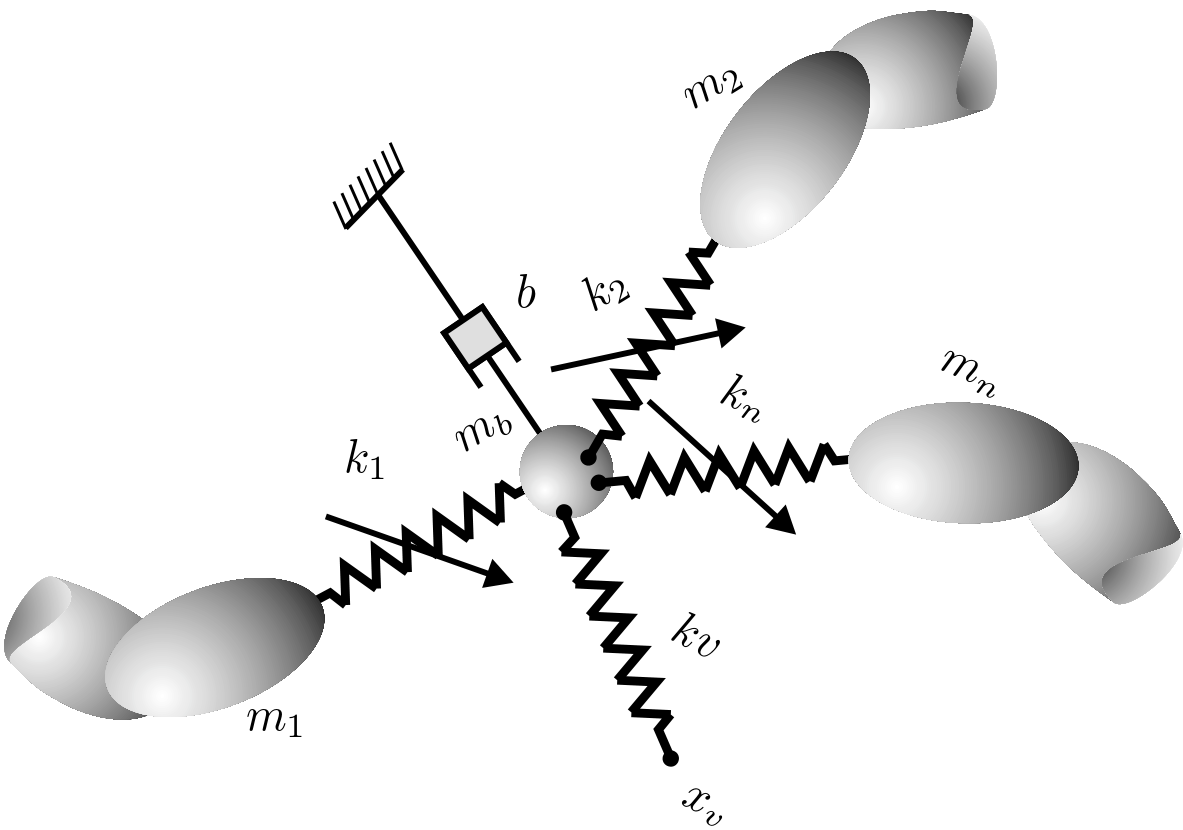
\includegraphics[width=0.8\textwidth]{IPCsprings.png}
	\caption[Structure of the IPC]{Structure of the IPC \cite{Stramigioli_99}}
	\label{FIG:IPCsprings}
\end{figure}
Starting point for the controller design is the virtual object. It is already given by equation (\ref{EQ:PHSinertia}). Springs to environment and manipulators exert wrenches on the object, in terms of port-Hamiltonian representation they are connected through the control port. The inertias of the manipulators should be equal to their real equivalents. Inertia re-shaping, using a local feed-back linearising compensation for the robot, can lead to infinite energy supply \cite{Stramigioli_01} and would thus violate passivity. In the absence of feed-back linearising the robot exhibits its internal dynamics at the end-effector. Therefore the inertia and Coriolis terms of the manipulators are configuration dependent. For the sake of simplicity we will omit this dependency in the following. Moreover the assume the robots to be gravity compensated and use the simpler port-Hamiltonian inertia representation of equation (\ref{EQ:PHSsimpleinertia}).    \\

From a geometric point of view the object-environment spring directly connects to the virtual object frame $\Psi_b$. The other end is attached to the desired object position, denoted with frame $\Psi_v$. This desired object position is the main control objective, by means of this, the motion of the constrained robot-object system is directed. The representation in PHS form is:
\begin{eqnarray}
	\dot{H}_v^b = T_v^{b}H_v^b\\
	W_v^{b} = \frac{\partial V_{v,b}}{\partial H_v^b}(H_v^b)^T
\end{eqnarray}
Since we already have a spring relation between the virtual object and the inertial frame it is useful to split this spring into two springs: one between desired position and inertial frame and the other between inertial frame and object position: $H_v^b$ = $H_0^b H_v^0 $.\\
Additionally we have a spring connecting object and each of the $n$-manipulators. As stated before these are variable rest-length springs, to allow for contraction and widening of the formation. Therefore the springs do not connect to the object frame but to a additional supporting frame denoted by $\Psi_v(i)$, which is rigidly attached to $\Psi_b$. Clearly the frames $\Psi_v(i),\; i=1...N$ define the sphere of the virtual object. The springs are situated between the manipulators and the virtual object sphere: $H_{v(i)}^i$ The rest-length is between the sphere and the virtual object frame: $H_b^{v(i)}$, the set-up is illustrated in Fig. \ref{FIG:IPCobject}.
\begin{figure}
	\centering
		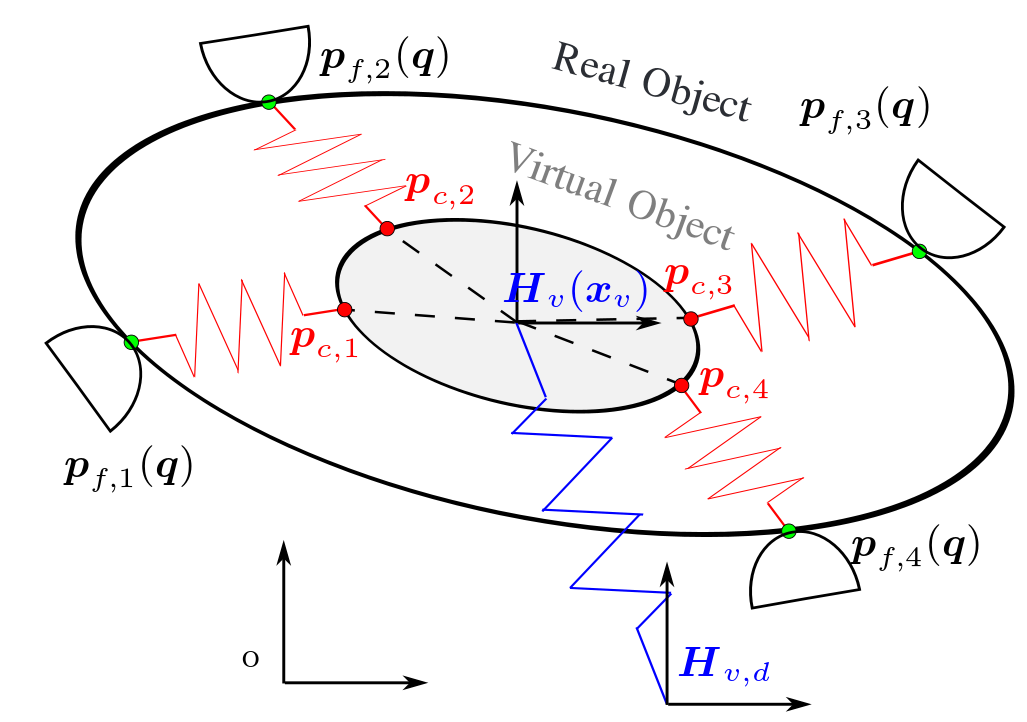
\includegraphics[width=0.8\textwidth]{IPCobjects.png}
		\caption[Virtual object and springs]{Virtual object and springs \cite{Wimboeck_08}}
		\label{FIG:IPCobject}
\end{figure}
% The spring forces act on the virtual object in the virtual contact points $\Psi_{v(i)}$. Therefore we need to map the spring forces to the object. This is done by the grasp map, a well known concept in cooperative manipulation (see e.g. \cite{CoopManipHandbook}). It relates both wrenches and motion between manipulators and object. For example the relation of the $i$-th spring to the object (angular) velocity $(\omega_b^T, v_b^T)^T$ is
%\[ \begin{pmatrix}\omega_{v(i)} \\ v_{v(i)}\end{pmatrix} = \begin{pmatrix}\omega_b  \\ v_b + p_{v(i)}^b \times \omega_b \end{pmatrix} \]
%We can combine this for all $ n $-manipulators and obtain the grasp matrix
%\[ G = \begin{pmatrix*}[l]
%S(p_{v(1)}^b) & I_3 \; \cdots \; S(p_{v(N)}^b) & I_3 \\ I_3 & 0_3 \; \cdots \; I_3 & 0_3 \end{pmatrix*} \]
%Wherein $S(\cdot)$ denotes the skew symmetric operation, defined in (\ref{EQ:skewsymmetricop}).
%The grasp matrix is a useful tool relating both twists and wrenches between object and manipulators:
%\begin{equation}
%W_b = GW \; , \; T = G^T T_b
%\end{equation}
%Where $W = (W_{v(1)}^T,...,W_{v(N)}^T)^T$ and $T = (T_{v(1)}^T,...,T_{v(N)}^T)^T$ are the stacked vectors of wrenches and twists respectively.\\
%Since we have defined geometric structure of the springs, we can give the PHS representation (see also (\ref{EQ:variablerestlengthspring}))
%\begin{eqnarray}\label{EQ:variablerestlengthspring}
%	\dot{H}_{v(i)}^i = \left( \begin{pmatrix}1 & Ad_{H_b^i}\end{pmatrix} \begin{pmatrix}T_b^{i} \\ T_{v(i)}^{b}\end{pmatrix} \right) H_{v(i)}^i\\
%	\begin{pmatrix}W_b^{i} \\ W_{v(i)}^{b}\end{pmatrix}  = \left( \begin{pmatrix}1 \\ Ad_{H_b^i}^T\end{pmatrix}  \frac{\partial V_{v(i),i}}{\partial H_{v(i)}^i} \right) (H_{v(i)}^i)^T 
%\end{eqnarray}
\subsubsection{Geometric interconnection of springs}
To combine all the presented equations to the full system as shown in Fig. \ref{FIG:IPCsprings}, we express the spring equations with respect to the inertial frame $\Psi_0$.
This is done for the virtual object spring by splitting the twists
\[T_b^v = (Ad_{H_0^v} \;\; -Ad_{H_0^v}) \begin{pmatrix} T_b^0 \\ T_v^0 \end{pmatrix}  \]
and the wrenches which obey the principle of action and reaction.
\[ \begin{pmatrix}W_b^{0} \\ W_v^{0}\end{pmatrix}  = 
\begin{pmatrix}Ad_{H_0^v}^T \\ -Ad_{H_0^v}^T \end{pmatrix} W_b^{v} \]
We can write the resulting PHS using the left translation (\ref{EQ:lefttranslation})
\begin{eqnarray}
	\dot{H}_b^v = H_b^v \left( (Ad_{H_0^b} \;\; -Ad_{H_0^b}) \begin{pmatrix} T_b^0 \\ T_v^0 \end{pmatrix}\right)   \\
	\begin{pmatrix}W_b^{0} \\ W_v^{0}\end{pmatrix}  = (H_b^v)^T \left(
	\begin{pmatrix}Ad_{H_0^b}^T \\ -Ad_{H_0^b}^T \end{pmatrix}
	\frac{\partial V_{v,b}}{\partial H_b^v} \right) 
\end{eqnarray} 
This is done with the springs connecting the $i$-th manipulator to the virtual object sphere in the same manner:
$T_{v(i)}^i = Ad_{H_0^i} T_b^0 - Ad_{H_0^i} T_i^0 + Ad_{H_b^i} T_{v(i)}^b $ Note that the twists and wrenches of rest-length changes are not expressed w.r.t. the inertial frame, since they represent a distinct power port. The resulting PHS for the spring connecting the $i$-th manipulator to the virtual object using the left translation is
\begin{eqnarray}
	\dot{H}_{v(i)}^i = H_{v(i)}^i \left( (Ad_{H_0^{v(i)}} \;\; -Ad_{H_0^{v(i)}} \;\; Ad_{H_b^{v(i)}}) \begin{pmatrix} T_b^0 \\ T_i^0 \\ T_{v(i)}^b \end{pmatrix}\right)   \\
	\begin{pmatrix}W_b^{0} \\ W_i^{0} \\ W_{v(i)}^b\end{pmatrix}  = (H_{v(i)}^i)^T \left(
	\begin{pmatrix}Ad_{H_0^{v(i)}}^T \\ -Ad_{H_0^{v(i)}}^T \\ Ad_{H_b^{v(i)}}^T\end{pmatrix}
	\frac{\partial V_{v(i),i}}{\partial H_{v(i)}^i} \right) 
\end{eqnarray}

For a simpler presentation we collect the twists and wrenches of the $n$ manipulator springs in a stacked vector notation
\[ T_i = \begin{pmatrix}T_1^0 \\ \vdots \\ T_N^0\end{pmatrix} \; , \; 
T_{rl} = \begin{pmatrix}T_{v(1)}^b \\ \vdots \\ T_{v(N)}^b\end{pmatrix} \; , \; W_i = \begin{pmatrix}W_1^0 \\ \vdots \\ W_N^0\end{pmatrix} \; , \;
W_{rl} = \begin{pmatrix}W_{v(1)}^b \\ \vdots \\ W_{v(N)}^b\end{pmatrix} \]
As a result we can combine all springs in a PHS
\begin{eqnarray}\label{EQ:PHScombinedsprings}
\underbrace{\begin{pmatrix}\dot{H}_{v(1)}^1 \\ \vdots \\ \dot{H}_{v(N)}^N \\ \dot{H}_b^v \end{pmatrix}}_{\dot{x}_s} =
\begin{pmatrix}
\phi_b & \phi_v & \phi_i & \phi_{rl}\end{pmatrix}
\begin{pmatrix}T_b^0 \\ T_v^0 \\ T_i \\ T_{rl}\end{pmatrix}
\\
\begin{pmatrix}W_b^0 \\ W_v^0 \\ W_i \\ W_{rl}\end{pmatrix} = 
\begin{pmatrix} \phi_b^T \\ \phi_v^T \\ \phi_i^T \\ \phi_{rl}^T\end{pmatrix} \frac{\partial V_s}{\partial x_s}
\end{eqnarray}
Where $V_s = V_{v,b} + \sum_{i=1}^N V_{v(i),i} $ is the sum of energy stored in the springs. The geometric interconnection of the springs is described by the matrices $\phi_b , \phi_v , \phi_i , \phi_{rl}$, their structure can be easily derived from the previous equations where every spring is described 
\[\phi_b = \begin{pmatrix}H_{v(1)}^1 Ad_{H_0^{v(1)}} \\ \vdots \\ H_{v(N)}^N Ad_{H_0^{v(N)}} \\ H_b^v Ad_{H_0^b}\end{pmatrix} \; , \;
\phi_v = \begin{pmatrix}0 \\ \vdots \\ 0 \\ - H_b^v Ad_{H_0^b}
\end{pmatrix} \],
\[\phi_i =  \begin{pmatrix} -H_{v(1)}^1 Ad_{H_0^{v(1)}} & \cdots & 0 \\ \vdots & \ddots & \vdots \\ 0 & \cdots & -H_{v(N)}^N Ad_{H_0^{v(N)}} \\
0 & \cdots & 0\end{pmatrix} \], \[
\phi_{rl} = \begin{pmatrix} H_{v(1)}^1 Ad_{H_b^{v(1)}} & \cdots & 0 \\ \vdots & \ddots & \vdots \\ 0 & \cdots & H_{v(N)}^N Ad_{H_b^{v(N)}} \\
0 & \cdots & 0\end{pmatrix} \]

\subsubsection{Interconnection of springs and inertias}

Having obtained a complete geometric description of the springs we can now add the inertias. The virtual object is attached to both, the environment spring and the manipulator springs. 
In the simulation the external forces acting on the inertia exclusively originate from these springs, thus $W_{ext}^b = - Ad_{H_b^0}^T W_b^0 $.
The wrench acting on the $i$-th manipulator stems from the $i$-th manipulator spring but also from the real manipulators: $ W_{ext}^i = -Ad_{H_i^0}^T W_i^0 + Ad_{H_i^0}^T W_{m(i)}^0$. Along with its dual twist we obtain the port that connects to the real robotic system, i.e. the robot control port. Concerning the twists we derive from equation (\ref{EQ:PHSinertia}) that $T_b^0 = Ad_{H_b^0}\frac{\partial V_{kg}}{\partial P_b^b}$. Equivalently the $i$-th manipulator wrench can be expressed as $T_i^0 = Ad_{H_i^0}\frac{\partial V_{k,i}}{\partial P_i^i} $. With this knowledge we can write the PHS representation of the complete control model. In order to keep the formulation compact we us the stacked state vector of the object inertia $x_b = ((H_b^0)^T \; (P_b^b)^T)^T$, the stacked vector of the spring states $x_S$ (defined in eq. (\ref{EQ:PHScombinedsprings})) and the vector of the manipulator inertia states $x_M = ((P_1^1)^T \; \cdots \; (P_N^N)^T)^T$. Analogously to the previous we write compactly for the manipulator wrenches $W_m = ((W_{m(1)}^0)^T \cdots (W_{m(N)}^0)^T)^T$. 
\begin{eqnarray}
\begin{pmatrix}\dot{x}_b \\ \dot{x}_S  \\ \dot{x}_M \end{pmatrix} =
\begin{pmatrix} J_B & -\phi_B^T & 0 \\ \phi_B & 0 & Ad_{H_i^0} \phi_i \\ 0 & -\phi_i^T Ad_{H_i^0}^T & C_M
 \end{pmatrix}
\begin{pmatrix}\frac{\partial V_{c}}{\partial x_b} \\ \frac{\partial V_{c}}{\partial x_S} \\ \frac{\partial V_{c}}{\partial x_M}\end{pmatrix} +
\begin{pmatrix}0 & 0 & 0\\ \phi_v & \phi_{rl} & 0\\ 0 & 0 & Ad_{H_n^0}^T\end{pmatrix} \begin{pmatrix} T_v^0 \\ T_{rl} \\ W_m\end{pmatrix}
\\
\begin{pmatrix}W_v^0 \\ W_{rl} \\ T_i\end{pmatrix} = \begin{pmatrix}0 & \phi_v^T & 0 \\ 0 & \phi_{rl}^T & 0 \\ 0 & 0 & Ad_{H_n^0}\end{pmatrix}
\begin{pmatrix}\frac{\partial V_{c}}{\partial x_b} \\ \frac{\partial V_{c}}{\partial x_S} \\ \frac{\partial V_{c}}{\partial x_M}\end{pmatrix}
\end{eqnarray}
Where $V_c = V_{v,b} + \sum_{i=1}^N [V_{v(i),i} + V_{k,i}] + V_{kg}$ is the combined energy function. $J_B$ is given in equation (\ref{EQ:PHSinertia}) and $C_M$ combines the Coriolis terms of all manipulators. The geometric interconnection matrix $\phi_B$ is composed by
\[ \phi_B = \begin{pmatrix} 0 \\ Ad_{H_b^0} \phi_b 
\end{pmatrix} \]

The reference inputs are $T_v$ and $T_{rl}$, allowing a high level control to specify twist trajectories for the object and the spring rest-lengths. Force-feedback is provided by their dual quantities. The robot system is connected with the port $(W_m,T_i)$, $W_m$ being the input and $T_i$ the output. Usually a robotic system expects the wrench to be the reference input and provides the resulting twist information. The concept of port-Hamiltonian systems allows for a simple inversion of causality by using a \emph{gyrator}. The power conserving relation is \[ \bar{W}_m = -T_i\]
\[ \bar{T_i} = W_m \]
The system is lossless, since no damping terms have been added so far.
\subsubsection{Adding damping}
The motion of the virtual object is damped with respect to the inertial frame $\Psi_0$. The object twist is already given in equation (\ref{EQ:PHSinertia}) and  the generates the damping wrench in object as defined in Subsection \ref{SSS:Dampers}. The resulting PHS representation of the virtual damped object is 
\[
\begin{pmatrix}\dot{H}_b^0 \\ \dot{P_b^b}\end{pmatrix} =
\underbrace{\begin{pmatrix} 0 & H_b^0  \\
- (H_b^0)^T & C_b-R_b\end{pmatrix}}_{J_B-R_B}
\begin{pmatrix}\frac{\partial V_{kg}}{\partial H_b^0} \\ \frac{\partial V_{kg}}{\partial P_b^b}\end{pmatrix}+
\begin{pmatrix}0 \\ W_{ext}^b\end{pmatrix} \]
\[T_b^0 = \begin{pmatrix}0 & Ad_{H_b^0}\end{pmatrix}
\begin{pmatrix}\frac{\partial V_{kg}}{\partial H_b^0} \\ \frac{\partial V_{kg}}{\partial P_b^b}\end{pmatrix}
\]
Damping for the manipulators shall be performed along the springs connecting the manipulator to the object. Recall that the twist of the $i$-th spring is 
\[ T_{v(i)}^i = Ad_{H_0^i} T_b^0 - Ad_{H_0^i} T_i^0 + Ad_{H_b^i} T_{v(i)}^b \]
The first component $T_b^0$ is already covered by the damping of the virtual object. The last component $T_{v(i)}^b$ is commanded by the operator and is executed unchanged. The remaining component $T_i^0$ relates to the motion of the manipulator inertia. Rewriting equation (\ref{EQ:PHSsimpleinertia}) we can give the damped manipulator inertia in PHS form
\[ 	\dot{P}_{i}^{i} = (C_{m(i)}-R_i) \frac{\partial V_{k,i}(P_{i}^{i})}{\partial P_{i}^{i}} + I_6 W_{ext}^{i} \]
\[	T_i^{i,0} = I_6 \frac{\partial V_{k,i}(P_i^i)}{\partial P_i^i} \]
It is easy to seen how the damping integrates into the complete system representation, therefore it will not be given here again.
\end{comment}

\section{Performance Comparison of control strategies}

To evaluate the presented controllers in an objective way, they are implemented in \emph{Simulink} and compared in terms of:
\begin{itemize}
	\item Trajectory tracking
	\item Dynamic behaviour
	\item Internal Forces
\end{itemize}

%Having explained the problem, and what others have done in similar situations, now explain your approach. Again, give a general overview of your design first, and then go into detail. The important part here is the concept of your work, not the actual implementation! Make sure that the document (particularly a thesis) is self-contained: It should be possible for a reader familiar with the general area to understand your design. Again, be forthright about the limitations of your design. Also, make sure you justify any shortcuts/limitations convincingly.

\subsection{Internal impedance control with feed-forward of the object dynamics}
De Pascali et al. \cite{DePascali_15} present combination of impedance control on manipulator/object level and feed-forward object dynamics. The internal impedance control relation (between object and manipulator) encompasses a spring and a parallel damper, inertia is used to feed-forward the desired acceleration: 
\begin{equation}
M_i \ddot{x}_i^d + D_i (\dot{x}_i^d - \dot{x}_i) + K_i(x_i^d,x_i) = h^x
\end{equation}
\textit{I know I have to use consistent notation and explain the variables, comes later ;)}
This avoids the necessity of either measuring manipulator acceleration or contact force.
Object dynamics is represented with a feed-forward term, mapped to the manipulators with a weighted pseudoinverse $ G^+ $ of the grasp matrix:
\begin{equation}
h^d = G^+ (M_o \ddot{x_o^d} + C_o \dot{x_o^d} + g_o)
\end{equation}
Note that this term is not an impedance relation and does not adjust if the environment hinders motion.
The combined control law is $ h^\Sigma = h^x + h^d $.\\
The set-up consists of four manipulators, distributed symmetrically around the object. In the first case translation in x-direction commanded. Results in Fig. \ref{FIG:abb1} show good tracking behaviour: no position errors in steady state and only small deviations from the desired values during transient phase. No internal stress is exerted on the object. Due to fast translation high manipulator forces occur.

%\begin{figure}[t]
%\begin{tikzpicture}
%	\begin{axis} [
%		ylabel = {$p_x$[m]},
%		xlabel = {t[s]},
%		minor y tick num = 1,
%		axis lines = left,
%		legend entries = {position, desired position},
%		legend style = {at={(axis cs:2.5, 0.7)}, anchor = north},
%		legend cell align=left,
%		grid = major,
%		height=5cm,
%		width=0.98\linewidth
%	]
%\addplot[red,]
%	table {/home/mangerer/MAgit/MA/Latex/plotdata/DePatransPosition.txt};
%\addplot[blue,]
%	table {/home/mangerer/MAgit/MA/Latex/plotdata/DePatransdesiredPosition.txt};
%%\draw[->, thick] (axis cs:5, 10) -- (axis cs:7, 9);
%%\draw[->, thick] (axis cs:15, 8) -- (axis cs:13.3, 6);
%%\draw[<->, thick] (axis cs:5.35, 5) -- (axis cs:5.35, 17);
%%\node at (axis cs:2.5,11){\small{\parbox{3.2cm}{Increased internal stress for $N_{h} \neq \{ 1{,}2{,}3\}$} }};
%%\node at (axis cs:15.5,9){\small{Placeholder}};
%\end{axis}
%\end{tikzpicture}
%\begin{tikzpicture}
%	\begin{axis} [
%		ylabel = {$v_x$[m/s]},
%		xlabel = {t[s]},
%		minor y tick num = 1,
%		axis lines = left,
%		legend entries = {velocity, desired velocity},
%		legend style = {at={(axis cs:0.8, -1)}, anchor = north},
%		legend cell align=left,
%		grid = major,
%		height=5cm,
%		width=0.98\linewidth
%	]
%\addplot[red,]
%	table {/home/mangerer/MAgit/MA/Latex/plotdata/DePatransVelocity.txt};
%\addplot[blue,]
%	table {/home/mangerer/MAgit/MA/Latex/plotdata/DepatransdesiredVelocity.txt};
%%\draw[->, thick] (axis cs:5, 10) -- (axis cs:7, 9);
%%\draw[->, thick] (axis cs:15, 8) -- (axis cs:13.3, 6);
%%\draw[<->, thick] (axis cs:5.35, 5) -- (axis cs:5.35, 17);
%%\node at (axis cs:2.5,11){\small{\parbox{3.2cm}{Increased internal stress for $N_{h} \neq \{ 1{,}2{,}3\}$} }};
%%\node at (axis cs:15.5,9){\small{Placeholder}};
%\end{axis}
%\end{tikzpicture}
%\begin{tikzpicture}
%	\begin{axis} [
%		ylabel = {f[N]},
%		xlabel = {t[s]},
%		minor y tick num = 1,
%		axis lines = left,
%		legend entries = {force $f_x$},
%		legend style = {at={(axis cs:2.5, 400)}, anchor = north},
%		legend cell align=left,
%		grid = major,
%		height=5cm,
%		width=0.98\linewidth
%	]
%\addplot[red,]
%	table {/home/mangerer/MAgit/MA/Latex/plotdata/DePatransManipWrench.txt};
%%\draw[->, thick] (axis cs:5, 10) -- (axis cs:7, 9);
%%\draw[->, thick] (axis cs:15, 8) -- (axis cs:13.3, 6);
%%\draw[<->, thick] (axis cs:5.35, 5) -- (axis cs:5.35, 17);
%%\node at (axis cs:2.5,11){\small{\parbox{3.2cm}{Increased internal stress for $N_{h} \neq \{ 1{,}2{,}3\}$} }};
%%\node at (axis cs:15.5,9){\small{Placeholder}};
%\end{axis}
%\end{tikzpicture}
%\caption[Internal force impedance control with feed-forward of the object dynamics: Translation]{Internal force impedance control with feed-forward of the object dynamics: Translation; Graphs from top: Position (desired/actual), Velocity (desired/actual), Force exerted by one manipulator, Internal wrench}
%\label{FIG:abb1}
%\end{figure}


In the second test case the object is rotated around the $ z $-axis. This is done at a significantly lower speed of at most 1 rad/s, thus the manipulator forces are smaller, desired and actual object trajectory cannot be distinguished in Fig. \ref{FIG:abb2}. However some small internal forces can be seen. Interestingly they are proportional to the simulation step size (running \emph{Simulink's ode3} solver), i.e. a ten-times smaller step size gives ten-times smaller internal forces. Internal forces are calculated based on the geometry in the last simulation step. The correlation between step size and values indicates that these forces are rather due to the discrete nature of the simulation than of the control law generating internal stress. Simulation of the constrained system dynamics as well as calculation of internal wrench is done as described in \cite{Erhart_15/2}.

%\begin{figure}[t]
%\begin{tikzpicture}
%	\begin{axis} [
%		ylabel = {$\Phi_z$[rad]},
%		xlabel = {t[s]},
%		minor y tick num = 1,
%		axis lines = left,
%		legend entries = {orientation, desired orientation},
%		legend style = {at={(axis cs:0.8, 1.2)}, anchor = north},
%		legend cell align=left,
%		grid = major,
%		height=5cm,
%		width=0.98\linewidth
%	]
%\addplot[red,]
%	table {/home/mangerer/MAgit/MA/Latex/plotdata/DePaOrientation.txt};
%\addplot[blue,]
%	table {/home/mangerer/MAgit/MA/Latex/plotdata/DePadesiredOrientation.txt};
%%\draw[->, thick] (axis cs:5, 10) -- (axis cs:7, 9);
%%\draw[->, thick] (axis cs:15, 8) -- (axis cs:13.3, 6);
%%\draw[<->, thick] (axis cs:5.35, 5) -- (axis cs:5.35, 17);
%%\node at (axis cs:2.5,11){\small{\parbox{3.2cm}{Increased internal stress for $N_{h} \neq \{ 1{,}2{,}3\}$} }};
%%\node at (axis cs:15.5,9){\small{Placeholder}};
%\end{axis}
%\end{tikzpicture}
%\begin{tikzpicture}
%	\begin{axis} [
%		ylabel = {$\omega_z$[rad/s]},
%		xlabel = {t[s]},
%		minor y tick num = 1,
%		axis lines = left,
%		legend entries = {angular velocity, des. ang. velocity},
%		legend style = {at={(axis cs:0.5, 0.95)}, anchor = north},
%		legend cell align=left,
%		grid = major,
%		height=5cm,
%		width=0.98\linewidth
%	]
%\addplot[red,]
%	table {/home/mangerer/MAgit/MA/Latex/plotdata/DePaangVelocity.txt};
%\addplot[blue,]
%	table {/home/mangerer/MAgit/MA/Latex/plotdata/DePadesiredangVelocity.txt};
%\end{axis}
%\end{tikzpicture}
%\begin{tikzpicture}
%	\begin{axis} [
%		ylabel = {f[N],m[Nm]},
%		xlabel = {t[s]},
%		minor y tick num = 1,
%		axis lines = left,
%		legend entries = {force $f_x$, force $f_y$, torque $m_z$},
%		legend style = {at={(axis cs:0.35, -1)}, anchor = north},
%		legend cell align=left,
%		grid = major,
%		height=5cm,
%		width=0.98\linewidth
%	]
%\addplot[red,]
%	table {/home/mangerer/MAgit/MA/Latex/plotdata/DePaManipWrenchtx.txt};
%\addplot[blue,]
%	table {/home/mangerer/MAgit/MA/Latex/plotdata/DePaManipWrenchty.txt};
%	\addplot[green,]
%	table {/home/mangerer/MAgit/MA/Latex/plotdata/DePaManipWrenchrz.txt};\end{axis}
%\end{tikzpicture}
%\begin{tikzpicture}
%	\begin{axis} [
%		ylabel = {f[N],m[Nm]},
%		xlabel = {t[s]},
%		minor y tick num = 1,
%		axis lines = left,
%		legend entries = {force $f_{int,x}$, force $f_{int,y}$, torque $m_{int,z}$},
%		legend style = {at={(axis cs:2.6, 0.04)}, anchor = north},
%		legend cell align=left,
%		grid = major,
%		height=5cm,
%		width=0.98\linewidth
%	]
%\addplot[red,]
%	table {/home/mangerer/MAgit/MA/Latex/plotdata/DePaIntWrenchtx.txt};
%\addplot[blue,]
%	table {/home/mangerer/MAgit/MA/Latex/plotdata/DePaIntWrenchty.txt};
%	\addplot[green,]
%	table {/home/mangerer/MAgit/MA/Latex/plotdata/DePaIntWrenchrz.txt};\end{axis}
%\end{tikzpicture}
%	\caption[Internal force impedance control with feed-forward of the object dynamics: Rotation]{Internal force impedance control with feed-forward of the object dynamics: Rotation; Graphs from top: Orientation (desired/actual), Angular Velocity (desired/actual), Force exerted by one manipulator, Internal wrench}
%	\label{FIG:abb2}
%\end{figure}



\subsection{Internal and external impedance based reference trajectory generation}
Caccavale and Villani \cite{Caccavale_01} combine both internal and external impedance control. With external we mean a compliant relation between object and (external) environment. The architecture is cascaded, consisting of a two level reference trajectory generation and a motion control loop below. On top-level an impedance relation between object and environment is used to generate a compliant trajectory subject to environmental forces:
\begin{equation}
\alpha M_o(\ddot{x}_o^d - \ddot{x}_o^r)  + D_o(\dot{x}_o^d - \dot{x}_o^r) + K_o(x_o^d,x_o^r)  = h_{env}
\end{equation}
The constant $ \alpha $ scales the object inertia proportionally to a desired value.
The control output is the reference object acceleration $ \ddot{x}_o^r $, $ h_{env} $ is an input. This is sometimes called admittance control, admittance being the inverse of impedance. $ h_{env} $ has to be known, but is not easily measured in a practical set-up. Recalling (\ref{EQ:ObjectDynamics}) the environmental forces can be expressed as:
\begin{equation}
h_{env} =  M_o \ddot{x}_o^r + C_o \dot{x}_o^r + g_o - G^\dagger h
\end{equation}
Herein $ G^\dagger $ is a generalized inverse of the grasp matrix, selecting the motion inducing components from the measured contact wrench $ h $. $ \dot{x}_o^r, x_o^r $ are calculated from $ \ddot{x}_o^r $ by integration.
From the compliant object trajectory ($ \ddot{x}_o^r,\dot{x}_o^r,x_o^r $) the desired trajectories of the manipulator ($ \ddot{x}_i^d,\dot{x}_i^d,x_i^d $) using the kinematic constraints. The reference manipulator trajectory, enforcing compliant behaviour between manipulators and object, is calculated from manipulator dynamics and internal forces: 
\begin{equation}
M_i(\ddot{x}_i^d - \ddot{x}_i^r) + D_i (\dot{x}_i^d - \dot{x}_i^r) + K_i(x_i^d,x_i^r) = VV^\dagger h
\end{equation}
The control output is the reference acceleration of the i-th manipulator $ \ddot{x}_i^r $, $ \dot{x}_i^r,x_i^r $ are obtained from integration. These variables are the inputs the inner motion control loop (PD-type). The strategy of compliant trajectories allows for high gains in the motion controller. Knowledge of object dynamics and measurement of the contact wrenches is required.\\
Results for translational motion (see Fig. \ref{FIG:abb3}) are very similar to that of the previous control scheme.

%\begin{figure}[t]
%\begin{tikzpicture}
%	\begin{axis} [
%		ylabel = {$p_x$[m]},
%		xlabel = {t[s]},
%		minor y tick num = 1,
%		axis lines = left,
%		legend entries = {position, desired position},
%		legend style = {at={(axis cs:2.5, 0.7)}, anchor = north},
%		legend cell align=left,
%		grid = major,
%		height=5cm,
%		width=0.98\linewidth
%	]
%\addplot[red,]
%	table {/home/mangerer/MAgit/MA/Latex/plotdata/CaVi_Position.txt};
%\addplot[blue,]
%	table {/home/mangerer/MAgit/MA/Latex/plotdata/CaVi_desiredPosition.txt};
%\end{axis}
%\end{tikzpicture}
%\begin{tikzpicture}
%	\begin{axis} [
%		ylabel = {$v_x$[m/s]},
%		xlabel = {t[s]},
%		minor y tick num = 1,
%		axis lines = left,
%		legend entries = {velocity, desired velocity},
%		legend style = {at={(axis cs:0.8, -1)}, anchor = north},
%		legend cell align=left,
%		grid = major,
%		height=5cm,
%		width=0.98\linewidth
%	]
%\addplot[red,]
%	table {/home/mangerer/MAgit/MA/Latex/plotdata/CaVi_Velocity.txt};
%\addplot[blue,]
%	table {/home/mangerer/MAgit/MA/Latex/plotdata/CaVi_desiredVelocity.txt};
%\end{axis}
%\end{tikzpicture}
%\begin{tikzpicture}
%	\begin{axis} [
%		ylabel = {f[N]},
%		xlabel = {t[s]},
%		minor y tick num = 1,
%		axis lines = left,
%		legend entries = {force $f_x$},
%		legend style = {at={(axis cs:2.5, 400)}, anchor = north},
%		legend cell align=left,
%		grid = major,
%		height=5cm,
%		width=0.98\linewidth
%	]
%\addplot[red,]
%	table {/home/mangerer/MAgit/MA/Latex/plotdata/CaVi_trans_ManipulatorWrench_tx.txt};
%\end{axis}
%\end{tikzpicture}
%\caption[Internal and external impedance based reference trajectory generation: Translation]{Internal and external impedance based reference trajectory generation: Translation; Graphs from top: Position (desired/actual), Velocity (desired/actual), Force exerted by one manipulator, Internal wrench}
%\label{FIG:abb3}
%\end{figure}


When it comes to rotation, higher internal forces can be observed in Fig. \ref{FIG:abb4}. In this case they are not influenced by numerical parameters of the simulation.

%\begin{figure}[t]
%\begin{tikzpicture}
%	\begin{axis} [
%		ylabel = {$\Phi_z$[rad]},
%		xlabel = {t[s]},
%		minor y tick num = 1,
%		axis lines = left,
%		legend entries = {orientation, desired orientation},
%		legend style = {at={(axis cs:0.8, 1.2)}, anchor = north},
%		legend cell align=left,
%		grid = major,
%		height=5cm,
%		width=0.98\linewidth
%	]
%\addplot[red,]
%	table {/home/mangerer/MAgit/MA/Latex/plotdata/CaVi_Orientation.txt};
%\addplot[blue,]
%	table {/home/mangerer/MAgit/MA/Latex/plotdata/CaVi_desired Orientation.txt};
%%\draw[->, thick] (axis cs:5, 10) -- (axis cs:7, 9);
%%\draw[->, thick] (axis cs:15, 8) -- (axis cs:13.3, 6);
%%\draw[<->, thick] (axis cs:5.35, 5) -- (axis cs:5.35, 17);
%%\node at (axis cs:2.5,11){\small{\parbox{3.2cm}{Increased internal stress for $N_{h} \neq \{ 1{,}2{,}3\}$} }};
%%\node at (axis cs:15.5,9){\small{Placeholder}};
%\end{axis}
%\end{tikzpicture}
%\begin{tikzpicture}
%	\begin{axis} [
%		ylabel = {$\omega_z$[rad/s]},
%		xlabel = {t[s]},
%		minor y tick num = 1,
%		axis lines = left,
%		legend entries = {angular velocity, des. ang. velocity},
%		legend style = {at={(axis cs:0.5, 0.95)}, anchor = north},
%		legend cell align=left,
%		grid = major,
%		height=5cm,
%		width=0.98\linewidth
%	]
%\addplot[red,]
%	table {/home/mangerer/MAgit/MA/Latex/plotdata/CaVi_Angular Velocity.txt};
%\addplot[blue,]
%	table {/home/mangerer/MAgit/MA/Latex/plotdata/CaVi_desired ang velocity.txt};
%\end{axis}
%\end{tikzpicture}
%\begin{tikzpicture}
%	\begin{axis} [
%		ylabel = {f[N],m[Nm]},
%		xlabel = {t[s]},
%		minor y tick num = 1,
%		axis lines = left,
%		legend entries = {force $f_x$, force $f_y$, torque $m_z$},
%		legend style = {at={(axis cs:0.35, -1)}, anchor = north},
%		legend cell align=left,
%		grid = major,
%		height=5cm,
%		width=0.98\linewidth
%	]
%\addplot[red,]
%	table {/home/mangerer/MAgit/MA/Latex/plotdata/CaVirot_Manipulator Wrench_tx.txt};
%\addplot[blue,]
%	table {/home/mangerer/MAgit/MA/Latex/plotdata/CaVirot_Manipulator Wrench_ty.txt};
%	\addplot[green,]
%	table {/home/mangerer/MAgit/MA/Latex/plotdata/CaVirot_Manipulator Wrench_rz.txt};\end{axis}
%\end{tikzpicture}
%\begin{tikzpicture}
%	\begin{axis} [
%		ylabel = {f[N],m[Nm]},
%		xlabel = {t[s]},
%		minor y tick num = 1,
%		axis lines = left,
%		legend entries = {force $f_{int,x}$, force $f_{int,y}$, torque $m_{int,z}$},
%		legend style = {at={(axis cs:2.6, 0.04)}, anchor = north},
%		legend cell align=left,
%		grid = major,
%		height=5cm,
%		width=0.98\linewidth
%	]
%\addplot[red,]
%	table {/home/mangerer/MAgit/MA/Latex/plotdata/CaVirot_Internal Wrench_tx.txt};
%\addplot[blue,]
%	table {/home/mangerer/MAgit/MA/Latex/plotdata/CaVirot_Internal Wrench_ty.txt};
%	\addplot[green,]
%	table {/home/mangerer/MAgit/MA/Latex/plotdata/CaVirot_Internal Wrench_rz.txt};\end{axis}
%\end{tikzpicture}
%\caption[Internal and external impedance based reference trajectory generation: Rotation]{Internal and external impedance based reference trajectory generation: Rotation; Graphs from top: Orientation (desired/actual), Angular Velocity (desired/actual), Force exerted by one manipulator, Internal wrench}
%\label{FIG:abb4}
%\end{figure}


This architecture in contrast to the previous makes use of measured contact wrenches. Contact wrench as measured can be obtained from the constrained system simulation. As described in \cite{CoopManipHandbook} this wrench is than decomposed by kineostatic filters in internal and external components. In this simulation this not cancel out undesired internal stress but magnifies it: when the contact wrench is not fed back and set to zero in the internal force impedance controller, results are slightly better. Note that the simulation represents an ideal case, where all parameters are exactly known and no deviations in grasp positions occur. Behavior in a real experiment may be different and this observation does not mean that the kineostatic-filtered feed-back of contact wrench is unjustified in general.



\subsection{Intrinsically Passive Controller (IPC)}
Introduced by Stramigioli \cite{Stramigioli_01} and implemented by Wimb\"ock et al. \cite{Wimboeck_08}, the architecture has been detailed throughout this work. In contrast to Stramigioli dampers are used in parallel with the manipulator springs and in contrast to Wimb\"ock all springs have 6-DoF. Simulation results for pure translation can be seen in Fig. \ref{FIG:DIPCtrans}. The object trajectory falls slightly behind the reference input, the dynamic behaviour is inferior to the previous approaches. Despite very stiff springs the magnitude of force seen in the previous approaches is not reached. No internal forces can be observed.

%\begin{figure}[t]
%\begin{tikzpicture}
%	\begin{axis} [
%		ylabel = {$p_x$[m]},
%		xlabel = {t[s]},
%		minor y tick num = 1,
%		axis lines = left,
%		legend entries = {position,desired position},
%		legend style = {at={(axis cs:2.6, 0.7)}, anchor = north},
%		legend cell align=left,
%		grid = major,
%		height=5cm,
%		width=0.98\linewidth
%	]
%\addplot[red,]
%	table {/home/mangerer/MAgit/MA/Latex/plotdata/DIPCtransPosition.txt};
%\addplot[blue,]
%	table {/home/mangerer/MAgit/MA/Latex/plotdata/DIPCtransdesiredPosition.txt};
%\end{axis}
%\end{tikzpicture}
%\begin{tikzpicture}
%	\begin{axis} [
%		ylabel = {$v_x$[m]},
%		xlabel = {t[s]},
%		minor y tick num = 1,
%		axis lines = left,
%		legend entries = {velocity,desired velocity},
%		legend style = {at={(axis cs:2.6, -2.7)}, anchor = north},
%		legend cell align=left,
%		grid = major,
%		height=5cm,
%		width=0.98\linewidth
%	]
%\addplot[red,]
%	table {/home/mangerer/MAgit/MA/Latex/plotdata/DIPCtransVelocity.txt};
%\addplot[blue,]
%	table {/home/mangerer/MAgit/MA/Latex/plotdata/DIPCtransdesiredVelocity.txt};
%\end{axis}
%\end{tikzpicture}
%\begin{tikzpicture}
%	\begin{axis} [
%		ylabel = {f[N]},
%		xlabel = {t[s]},
%		minor y tick num = 1,
%		axis lines = left,
%		legend entries = {force $f_x$},
%		legend style = {at={(axis cs:2.6, 500)}, anchor = north},
%		legend cell align=left,
%		grid = major,
%		height=5cm,
%		width=0.98\linewidth
%	]
%\addplot[red,]
%	table {/home/mangerer/MAgit/MA/Latex/plotdata/DIPCtransManipulatorWrenchtx.txt};
%\end{axis}
%\end{tikzpicture}
%\vspace{-10pt}
%	\caption[IPC: Translation]{Intrinsically Passive Controller: Translation; Graphs from top: Position (desired/actual), Velocity (desired/actual), Force exerted by one manipulator}
%	\label{FIG:DIPCtrans}
%\end{figure}

When it comes to rotation (see Fig. \ref{FIG:DIPCrot}) again the dynamic behaviour falls short of the two other approaches, while the manipulator wrench is higher. Significant internal wrenches are present, they amount up to 50\% of the manipulator wrenches.


%\begin{figure}[t]
%\begin{tikzpicture}
%	\begin{axis} [
%		ylabel = {$\Phi_z$[rad]},
%		xlabel = {t[s]},
%		minor y tick num = 1,
%		axis lines = left,
%		legend entries = {orientation, desired orientation},
%		legend style = {at={(axis cs:0.8, 1.2)}, anchor = north},
%		legend cell align=left,
%		grid = major,
%		height=5cm,
%		width=0.98\linewidth
%	]
%\addplot[red,]
%	table {/home/mangerer/MAgit/MA/Latex/plotdata/DIPCorientation.txt};
%\addplot[blue,]
%	table {/home/mangerer/MAgit/MA/Latex/plotdata/DIPCdesiredOrientation.txt};
%%\draw[->, thick] (axis cs:5, 10) -- (axis cs:7, 9);
%%\draw[->, thick] (axis cs:15, 8) -- (axis cs:13.3, 6);
%%\draw[<->, thick] (axis cs:5.35, 5) -- (axis cs:5.35, 17);
%%\node at (axis cs:2.5,11){\small{\parbox{3.2cm}{Increased internal stress for $N_{h} \neq \{ 1{,}2{,}3\}$} }};
%%\node at (axis cs:15.5,9){\small{Placeholder}};
%\end{axis}
%\end{tikzpicture}
%\begin{tikzpicture}
%	\begin{axis} [
%		ylabel = {$\omega_z$[rad/s]},
%		xlabel = {t[s]},
%		minor y tick num = 1,
%		axis lines = left,
%		legend entries = {angular velocity, des. ang. velocity},
%		legend style = {at={(axis cs:0.5, 0.95)}, anchor = north},
%		legend cell align=left,
%		grid = major,
%		height=5cm,
%		width=0.98\linewidth
%	]
%\addplot[red,]
%	table {/home/mangerer/MAgit/MA/Latex/plotdata/DIPCAngVelocity.txt};
%\addplot[blue,]
%	table {/home/mangerer/MAgit/MA/Latex/plotdata/DIPCdesiredAngVelocity.txt};
%\end{axis}
%\end{tikzpicture}
%\begin{tikzpicture}
%	\begin{axis} [
%		ylabel = {f[N],m[Nm]},
%		xlabel = {t[s]},
%		minor y tick num = 1,
%		axis lines = left,
%		legend entries = {force $f_x$, force $f_y$, torque $m_z$},
%		legend style = {at={(axis cs:0.35, -1)}, anchor = north},
%		legend cell align=left,
%		grid = major,
%		height=5cm,
%		width=0.98\linewidth
%	]
%\addplot[red,]
%	table {/home/mangerer/MAgit/MA/Latex/plotdata/DIPCManipulatorWrenchtx.txt};
%\addplot[blue,]
%	table {/home/mangerer/MAgit/MA/Latex/plotdata/DIPCManipulatorWrenchty.txt};
%	\addplot[green,]
%	table {/home/mangerer/MAgit/MA/Latex/plotdata/DIPCManipulatorWrenchrz.txt};\end{axis}
%\end{tikzpicture}
%\begin{tikzpicture}
%	\begin{axis} [
%		ylabel = {f[N],m[Nm]},
%		xlabel = {t[s]},
%		minor y tick num = 1,
%		axis lines = left,
%		legend entries = {force $f_{int,x}$, force $f_{int,y}$, torque $m_{int,z}$},
%		legend style = {at={(axis cs:2.6, 0.04)}, anchor = north},
%		legend cell align=left,
%		grid = major,
%		height=5cm,
%		width=0.98\linewidth
%	]
%\addplot[red,]
%	table {/home/mangerer/MAgit/MA/Latex/plotdata/DIPCInternalWrenchtx.txt};
%\addplot[blue,]
%	table {/home/mangerer/MAgit/MA/Latex/plotdata/DIPCInternalWrenchty.txt};
%	\addplot[green,]
%	table {/home/mangerer/MAgit/MA/Latex/plotdata/DIPCInternalWrenchrz.txt};\end{axis}
%\end{tikzpicture}
%\vspace{-10pt}
%\caption[IPC: Rotation]{Intrinsically Passive Controller: Rotation; Graphs from top: Orientation (desired/actual), Angular Velocity (desired/actual), Force exerted by one manipulator, Internal wrench}
%	\label{FIG:DIPCrot}
%\end{figure}


%\section{Implementation}
%
%
%In many (not all cases) there is a clear difference between the general approach (design) and its implementation in your particular circumstances. The design may be more general than what you can do given time and resources. Or you have developed a general design, and are now implementing a prototype on particular hardware. Give all required details. It should be possible to understand all this without referring to the source code. 
%
%This will, in general, include extracts of actual algorithms and hardware components used. Don't list pages of C code, an electronic copy of the source will accompany the submission and should be available to the marker, so there's no point in killing extra trees to put it into the report. Source code, if included at all, goes into the appendix and not the main document.
%
%Make sure you describe your implementation in enough detail. Someone who has nothing else but your thesis report to go by should be able to repeat your work, and arrive at essentially the same implementation. Reproducibility is an important component of scientific work. Also, clearly state the limitations of your implementation, and justify them.
%
%\section{Experimental Results}
%
%A thesis almost always has an experimental part, typically some comparison to other approaches. Benchmarking takes time, for running the experiments, but also for thinking them up in the first place, and for analysing the results. Plan accordingly to spend enough time here!
%
%Think about what makes sense to measure, what you want to learn from your measurements. Think about what is really the relevant contribution of your thesis, and how you can prove that you have achieved your goals. Think about what you can measure in order to get a good insight into the performance of various aspects of your design, how you can distinguish between systematic and accidental effects, how you can convince yourself that your results are right. If you get surprising results, don't just say "surprise, surprise, performance isn't as good as hoped". Find out why. Surprises without explanation indicate either that you are clueless about what's going on, or that you have made a mistake. Unconvincing results, therefore, tend to imply unconvincing marks. 
%
%\paragraph{Statistics:} Measurements always have statistical (sampling) errors. Owing to the deterministic nature of simulations these are sometimes very small, as disturbing factors can be designed. However, the reader should be given an indication of how statistically significant the results are. This is done by providing at least a standard deviation in addition to averages. Whenever the results of several runs are averaged, a standard deviation can (and must) be supplied. After all, you average to reduce statistical errors.
%
%The reproducibility argument applies here just as much as for the implementation. Give enough detail on what you measure, and how you measure it, so that someone who has your implementation (but not your test code) or has re-done your implementation independently, should be able to repeat your measurements and arrive at essentially the same results. In some cases, results seem outright wrong in a thesis. In those cases, not enough detail is provided to allow the supervisor/reader to pinpoint the likely source of the error. Often the cause is systematic errors resulting from an incorrect measurement technique. If it seems wrong, and the text doesn't convince the reader that it is not wrong, the reader will assume that it is wrong.
%
%\section{Discussion}
%
%Discuss and explain your results. Show how they support your thesis (or, if they don't, give a convincing explanation). It is important to separate objective facts clearly from their discussion (which is bound to contain subjective opinion). If the reader doesn't understand your results, reconsider if you have managed to extract the core information and explain it in a straightforward way.

%_______________________________________________



%_____Zusammenfassung, Ausblick_________________________________
\chapter{Conclusion}
  

%Don't leave it at the discussion: discuss what you/the reader can learn from the results. Draw some real conclusions. Separate discussion/interpretation of the results clearly from the conclusions you draw from them. (So-called "conclusion creep" tends to upset reviewers. It means surrendering your scientific objectivity.) Identify all shortcomings/limitations of your work, and discuss how they could be fixed ("future work"). It is not a sign of weakness of your work, if you clearly analyse and state the limitations. Informed readers will notice them anyway and draw their own conclusions, if not addressed properly.
%
%\vspace{\baselineskip}
%Recap: don't stick to this structure at all cost. Also, remember that the thesis must be:
%
%\begin{itemize}
%	\item honest, stating clearly all limitations;
%	\item self--contained, don't write just for the locals, don't assume that the reader has read the same literature as you, don't let the reader work out the details for themselves.
%\end{itemize}
%
%
%
%This chapter is followed by the list of figures and the bibliography. If you are using acronyms, listing them (with the expanded full name) before the bibliography is also a good idea. The acronyms package helps with consistency and an automatic listing.


%_______________________________________________________________


%_____Abbildungsverzeichnis_________________________________
\cleardoublepage
\addcontentsline{toc}{chapter}{List of Figures} 
\listoffigures 	 %Abbildungsverzeichnis

%___________________________________________________________

%_____Literaturverzeichnis_________________________________
\cleardoublepage
\addcontentsline{toc}{chapter}{Bibliography}
\bibliography{mybib}{}
\bibliographystyle{alphaurl}
%__________________________________________________________


%_____License_________________________________
\cleardoublepage
\chapter*{License}
\markright{LICENSE}
This work is licensed under the Creative Commons Attribution 3.0 Germany
License. To view a copy of this license,
visit \href{http://creativecommons.org/licenses/by/3.0/de/}{http://creativecommons.org} or send a letter
to Creative Commons, 171 Second Street, Suite 300, San
Francisco, California 94105, USA.
%__________________________________________________________

\end{document}
